\documentclass[]{book}
\usepackage{lmodern}
\usepackage{amssymb,amsmath}
\usepackage{ifxetex,ifluatex}
\usepackage{fixltx2e} % provides \textsubscript
\ifnum 0\ifxetex 1\fi\ifluatex 1\fi=0 % if pdftex
  \usepackage[T1]{fontenc}
  \usepackage[utf8]{inputenc}
\else % if luatex or xelatex
  \ifxetex
    \usepackage{mathspec}
  \else
    \usepackage{fontspec}
  \fi
  \defaultfontfeatures{Ligatures=TeX,Scale=MatchLowercase}
\fi
% use upquote if available, for straight quotes in verbatim environments
\IfFileExists{upquote.sty}{\usepackage{upquote}}{}
% use microtype if available
\IfFileExists{microtype.sty}{%
\usepackage{microtype}
\UseMicrotypeSet[protrusion]{basicmath} % disable protrusion for tt fonts
}{}
\usepackage[margin=1in]{geometry}
\usepackage{hyperref}
\hypersetup{unicode=true,
            pdftitle={WholeBrain tutorials},
            pdfauthor={Daniel Fürth},
            pdfborder={0 0 0},
            breaklinks=true}
\urlstyle{same}  % don't use monospace font for urls
\usepackage{natbib}
\bibliographystyle{apalike}
\usepackage{color}
\usepackage{fancyvrb}
\newcommand{\VerbBar}{|}
\newcommand{\VERB}{\Verb[commandchars=\\\{\}]}
\DefineVerbatimEnvironment{Highlighting}{Verbatim}{commandchars=\\\{\}}
% Add ',fontsize=\small' for more characters per line
\usepackage{framed}
\definecolor{shadecolor}{RGB}{248,248,248}
\newenvironment{Shaded}{\begin{snugshade}}{\end{snugshade}}
\newcommand{\KeywordTok}[1]{\textcolor[rgb]{0.13,0.29,0.53}{\textbf{{#1}}}}
\newcommand{\DataTypeTok}[1]{\textcolor[rgb]{0.13,0.29,0.53}{{#1}}}
\newcommand{\DecValTok}[1]{\textcolor[rgb]{0.00,0.00,0.81}{{#1}}}
\newcommand{\BaseNTok}[1]{\textcolor[rgb]{0.00,0.00,0.81}{{#1}}}
\newcommand{\FloatTok}[1]{\textcolor[rgb]{0.00,0.00,0.81}{{#1}}}
\newcommand{\ConstantTok}[1]{\textcolor[rgb]{0.00,0.00,0.00}{{#1}}}
\newcommand{\CharTok}[1]{\textcolor[rgb]{0.31,0.60,0.02}{{#1}}}
\newcommand{\SpecialCharTok}[1]{\textcolor[rgb]{0.00,0.00,0.00}{{#1}}}
\newcommand{\StringTok}[1]{\textcolor[rgb]{0.31,0.60,0.02}{{#1}}}
\newcommand{\VerbatimStringTok}[1]{\textcolor[rgb]{0.31,0.60,0.02}{{#1}}}
\newcommand{\SpecialStringTok}[1]{\textcolor[rgb]{0.31,0.60,0.02}{{#1}}}
\newcommand{\ImportTok}[1]{{#1}}
\newcommand{\CommentTok}[1]{\textcolor[rgb]{0.56,0.35,0.01}{\textit{{#1}}}}
\newcommand{\DocumentationTok}[1]{\textcolor[rgb]{0.56,0.35,0.01}{\textbf{\textit{{#1}}}}}
\newcommand{\AnnotationTok}[1]{\textcolor[rgb]{0.56,0.35,0.01}{\textbf{\textit{{#1}}}}}
\newcommand{\CommentVarTok}[1]{\textcolor[rgb]{0.56,0.35,0.01}{\textbf{\textit{{#1}}}}}
\newcommand{\OtherTok}[1]{\textcolor[rgb]{0.56,0.35,0.01}{{#1}}}
\newcommand{\FunctionTok}[1]{\textcolor[rgb]{0.00,0.00,0.00}{{#1}}}
\newcommand{\VariableTok}[1]{\textcolor[rgb]{0.00,0.00,0.00}{{#1}}}
\newcommand{\ControlFlowTok}[1]{\textcolor[rgb]{0.13,0.29,0.53}{\textbf{{#1}}}}
\newcommand{\OperatorTok}[1]{\textcolor[rgb]{0.81,0.36,0.00}{\textbf{{#1}}}}
\newcommand{\BuiltInTok}[1]{{#1}}
\newcommand{\ExtensionTok}[1]{{#1}}
\newcommand{\PreprocessorTok}[1]{\textcolor[rgb]{0.56,0.35,0.01}{\textit{{#1}}}}
\newcommand{\AttributeTok}[1]{\textcolor[rgb]{0.77,0.63,0.00}{{#1}}}
\newcommand{\RegionMarkerTok}[1]{{#1}}
\newcommand{\InformationTok}[1]{\textcolor[rgb]{0.56,0.35,0.01}{\textbf{\textit{{#1}}}}}
\newcommand{\WarningTok}[1]{\textcolor[rgb]{0.56,0.35,0.01}{\textbf{\textit{{#1}}}}}
\newcommand{\AlertTok}[1]{\textcolor[rgb]{0.94,0.16,0.16}{{#1}}}
\newcommand{\ErrorTok}[1]{\textcolor[rgb]{0.64,0.00,0.00}{\textbf{{#1}}}}
\newcommand{\NormalTok}[1]{{#1}}
\usepackage{longtable,booktabs}
\usepackage{graphicx,grffile}
\makeatletter
\def\maxwidth{\ifdim\Gin@nat@width>\linewidth\linewidth\else\Gin@nat@width\fi}
\def\maxheight{\ifdim\Gin@nat@height>\textheight\textheight\else\Gin@nat@height\fi}
\makeatother
% Scale images if necessary, so that they will not overflow the page
% margins by default, and it is still possible to overwrite the defaults
% using explicit options in \includegraphics[width, height, ...]{}
\setkeys{Gin}{width=\maxwidth,height=\maxheight,keepaspectratio}
\IfFileExists{parskip.sty}{%
\usepackage{parskip}
}{% else
\setlength{\parindent}{0pt}
\setlength{\parskip}{6pt plus 2pt minus 1pt}
}
\setlength{\emergencystretch}{3em}  % prevent overfull lines
\providecommand{\tightlist}{%
  \setlength{\itemsep}{0pt}\setlength{\parskip}{0pt}}
\setcounter{secnumdepth}{5}
% Redefines (sub)paragraphs to behave more like sections
\ifx\paragraph\undefined\else
\let\oldparagraph\paragraph
\renewcommand{\paragraph}[1]{\oldparagraph{#1}\mbox{}}
\fi
\ifx\subparagraph\undefined\else
\let\oldsubparagraph\subparagraph
\renewcommand{\subparagraph}[1]{\oldsubparagraph{#1}\mbox{}}
\fi

%%% Use protect on footnotes to avoid problems with footnotes in titles
\let\rmarkdownfootnote\footnote%
\def\footnote{\protect\rmarkdownfootnote}

%%% Change title format to be more compact
\usepackage{titling}

% Create subtitle command for use in maketitle
\newcommand{\subtitle}[1]{
  \posttitle{
    \begin{center}\large#1\end{center}
    }
}

\setlength{\droptitle}{-2em}
  \title{WholeBrain tutorials}
  \pretitle{\vspace{\droptitle}\centering\huge}
  \posttitle{\par}
  \author{Daniel Fürth}
  \preauthor{\centering\large\emph}
  \postauthor{\par}
  \predate{\centering\large\emph}
  \postdate{\par}
  \date{2017-07-22}

\usepackage{booktabs}
\usepackage{amsthm}
\makeatletter
\def\thm@space@setup{%
  \thm@preskip=8pt plus 2pt minus 4pt
  \thm@postskip=\thm@preskip
}
\makeatother

\usepackage{amsthm}
\newtheorem{theorem}{Theorem}[chapter]
\newtheorem{lemma}{Lemma}[chapter]
\theoremstyle{definition}
\newtheorem{definition}{Definition}[chapter]
\newtheorem{corollary}{Corollary}[chapter]
\newtheorem{proposition}{Proposition}[chapter]
\theoremstyle{definition}
\newtheorem{example}{Example}[chapter]
\theoremstyle{remark}
\newtheorem*{remark}{Remark}
\begin{document}
\maketitle

{
\setcounter{tocdepth}{1}
\tableofcontents
}
\chapter{Preface}\label{preface}

TBA

\chapter{Introduction}\label{intro}

\chapter{Segment}\label{segment}

Segmentation.

\chapter{Registration}\label{registration}

TBA.

\chapter{Make web map}\label{make-web-map}

\section{Static web maps.}\label{static-web-maps.}

\chapter{3D reconstruction}\label{d-reconstruction}

Once you have processed more than one section you can collapse then into
a single tidy data frame that can be used for 3D reconstruction..

\chapter{Statistical analysis}\label{statistical-analysis}

\section{Handling data.}\label{handling-data.}

\section{Plotting.}\label{plotting.}

\section{Modeling.}\label{modeling.}

\chapter{Colocalization}\label{colocalization}

TBA.

\chapter{smFISH}\label{smfish}

TBA.

\chapter{Spatial transcriptomics.}\label{spatial-transcriptomics.}

\section{Load in the preprocessed
WholeBrain/ST-data.}\label{load-in-the-preprocessed-wholebrainst-data.}

First lets load the segmentation of individual spots (with polygon
contours) as well as their centroid (seg.spots list object) together
with segmentation of individual cell nuclei (cells) and the registration
object to the reference atlas (regi).

\begin{Shaded}
\begin{Highlighting}[]
\CommentTok{#load registration and segmentation output into R workingspace}
\KeywordTok{load}\NormalTok{(}\StringTok{'./data/spatial_transcriptomics/170605/D2_S4_seg_and_reg.RData'}\NormalTok{)}
\end{Highlighting}
\end{Shaded}

With this you will have the following list objects in your working
space:

\begin{itemize}
\tightlist
\item
  \texttt{seg.spots} output from
  \texttt{segmentation(image,\ get.contour=TRUE)} on the Cy3 spot image.
\item
  \texttt{cells} output from \texttt{segmentation(image)} on the H\&E
  image (individual nuclei and tissue contour).
\item
  \texttt{regi} output from \texttt{registration(image,\ coordinate=X)}
\end{itemize}

Check that this is true by typing \texttt{ls()} in the R console to
check objects in your working space.

\begin{Shaded}
\begin{Highlighting}[]
\KeywordTok{ls}\NormalTok{()}
\end{Highlighting}
\end{Shaded}

\begin{verbatim}
## [1] "cells"     "regi"      "seg.spots"
\end{verbatim}

You can try to plot all individual cell nuclei and all segmented spots
by the following commands:

\begin{Shaded}
\begin{Highlighting}[]
\CommentTok{#helper function to plot spots as polygons}
\NormalTok{polygon.spot<-function(contour.ID, }\DataTypeTok{alpha=}\FloatTok{0.2}\NormalTok{)\{}
  \NormalTok{x<-seg.spots$soma$contour.x[}\KeywordTok{which}\NormalTok{(seg.spots$soma$contour.ID==contour.ID)]}
  \NormalTok{y<-seg.spots$soma$contour.y[}\KeywordTok{which}\NormalTok{(seg.spots$soma$contour.ID==contour.ID)]}
  \KeywordTok{polygon}\NormalTok{(x,y, }\DataTypeTok{border=}\StringTok{'darkred'}\NormalTok{, }\DataTypeTok{col=}\KeywordTok{rgb}\NormalTok{(}\DecValTok{1}\NormalTok{,}\DecValTok{0}\NormalTok{,}\DecValTok{0}\NormalTok{, alpha))}
\NormalTok{\}}
\CommentTok{#helper function to plot atlas regions in the tissue}
\NormalTok{polygon.atlas<-function(contour.ID)\{}
  \CommentTok{#scale fatcor to upsample to original image}
  \NormalTok{scale.factor<-}\KeywordTok{mean}\NormalTok{(}\KeywordTok{c}\NormalTok{(regi$transformationgrid$height,regi$transformationgrid$width)/}\KeywordTok{dim}\NormalTok{(regi$transformationgrid$mx))}
  \NormalTok{for(i in }\DecValTok{1}\NormalTok{:}\DecValTok{2}\NormalTok{)\{}
    \NormalTok{region<-regi$atlas$outlines[[contour.ID]][}\KeywordTok{c}\NormalTok{(}\DecValTok{2}\NormalTok{*}\DecValTok{1-1}\NormalTok{,}\DecValTok{2}\NormalTok{*}\DecValTok{1}\NormalTok{)+}\DecValTok{4}\NormalTok{]}
    \KeywordTok{names}\NormalTok{(region)<-}\KeywordTok{c}\NormalTok{(}\StringTok{'x'}\NormalTok{, }\StringTok{'y'}\NormalTok{)}
    \KeywordTok{polygon}\NormalTok{(region$x*scale.factor, region$y*scale.factor, }\DataTypeTok{border=}\StringTok{'purple'}\NormalTok{)}
  \NormalTok{\}}
\NormalTok{\}}
\end{Highlighting}
\end{Shaded}

Then lets plot this with:

\begin{Shaded}
\begin{Highlighting}[]
\CommentTok{#do some plotting}
\KeywordTok{par}\NormalTok{(}\DataTypeTok{mfrow=}\KeywordTok{c}\NormalTok{(}\DecValTok{1}\NormalTok{,}\DecValTok{2}\NormalTok{), }\DataTypeTok{mar=}\KeywordTok{c}\NormalTok{(}\DecValTok{0}\NormalTok{,}\DecValTok{0}\NormalTok{,}\DecValTok{0}\NormalTok{,}\DecValTok{0}\NormalTok{))}
\CommentTok{#plot cell nuclei as black small spots}
\KeywordTok{plot}\NormalTok{(cells$soma$x, cells$soma$y, }\DataTypeTok{cex=}\FloatTok{0.08}\NormalTok{, }\DataTypeTok{pch=}\DecValTok{16}\NormalTok{, }\DataTypeTok{ylim=}\KeywordTok{c}\NormalTok{(}\KeywordTok{max}\NormalTok{(cells$soma$y),}\DecValTok{0}\NormalTok{), }\DataTypeTok{asp=}\DecValTok{1}\NormalTok{, }\DataTypeTok{ylab=}\StringTok{''}\NormalTok{, }\DataTypeTok{xlab=}\StringTok{''}\NormalTok{, }\DataTypeTok{axes=}\OtherTok{FALSE}\NormalTok{)}
\CommentTok{#plot region outlines}
\KeywordTok{invisible}\NormalTok{(}\KeywordTok{lapply}\NormalTok{(}\DecValTok{1}\NormalTok{:regi$atlas$numRegions, polygon.atlas))}
\CommentTok{#plot spots as polygons}
\KeywordTok{invisible}\NormalTok{(}\KeywordTok{lapply}\NormalTok{(}\KeywordTok{unique}\NormalTok{(seg.spots$soma$contour.ID), polygon.spot))}
\CommentTok{#make a ROI for closeup}
\NormalTok{roi<-}\KeywordTok{list}\NormalTok{(}\DataTypeTok{x=}\KeywordTok{median}\NormalTok{(cells$soma$x)+}\KeywordTok{c}\NormalTok{(-}\DecValTok{1000}\NormalTok{,}\DecValTok{1000}\NormalTok{), }\DataTypeTok{y=}\KeywordTok{median}\NormalTok{(cells$soma$y)+}\KeywordTok{c}\NormalTok{(-}\DecValTok{1000}\NormalTok{,}\DecValTok{1000}\NormalTok{))}
\KeywordTok{polygon}\NormalTok{(}\KeywordTok{c}\NormalTok{(roi$x, }\KeywordTok{rev}\NormalTok{(roi$x)), }\KeywordTok{rep}\NormalTok{(roi$y, }\DataTypeTok{each=}\DecValTok{2}\NormalTok{), }\DataTypeTok{border=}\StringTok{'green3'}\NormalTok{, }\DataTypeTok{lwd=}\DecValTok{2}\NormalTok{)}
\CommentTok{#plot closeup}
\CommentTok{#plot cell nuclei as black small spots}
\KeywordTok{plot}\NormalTok{(cells$soma$x, cells$soma$y, }\DataTypeTok{cex=}\DecValTok{1}\NormalTok{, }\DataTypeTok{pch=}\DecValTok{16}\NormalTok{, }\DataTypeTok{ylim=}\NormalTok{roi$y,  }\DataTypeTok{xlim=}\NormalTok{roi$x, }\DataTypeTok{asp=}\DecValTok{1}\NormalTok{, }\DataTypeTok{ylab=}\StringTok{''}\NormalTok{, }\DataTypeTok{xlab=}\StringTok{''}\NormalTok{, }\DataTypeTok{axes=}\OtherTok{FALSE}\NormalTok{)}
\KeywordTok{polygon}\NormalTok{(}\KeywordTok{c}\NormalTok{(roi$x, }\KeywordTok{rev}\NormalTok{(roi$x)), }\KeywordTok{rep}\NormalTok{(roi$y, }\DataTypeTok{each=}\DecValTok{2}\NormalTok{), }\DataTypeTok{border=}\StringTok{'green3'}\NormalTok{, }\DataTypeTok{lwd=}\DecValTok{2}\NormalTok{)}
\KeywordTok{box}\NormalTok{()}
\CommentTok{#plot spots as polygons}
\KeywordTok{invisible}\NormalTok{(}\KeywordTok{lapply}\NormalTok{(}\KeywordTok{unique}\NormalTok{(seg.spots$soma$contour.ID), polygon.spot))}
\end{Highlighting}
\end{Shaded}

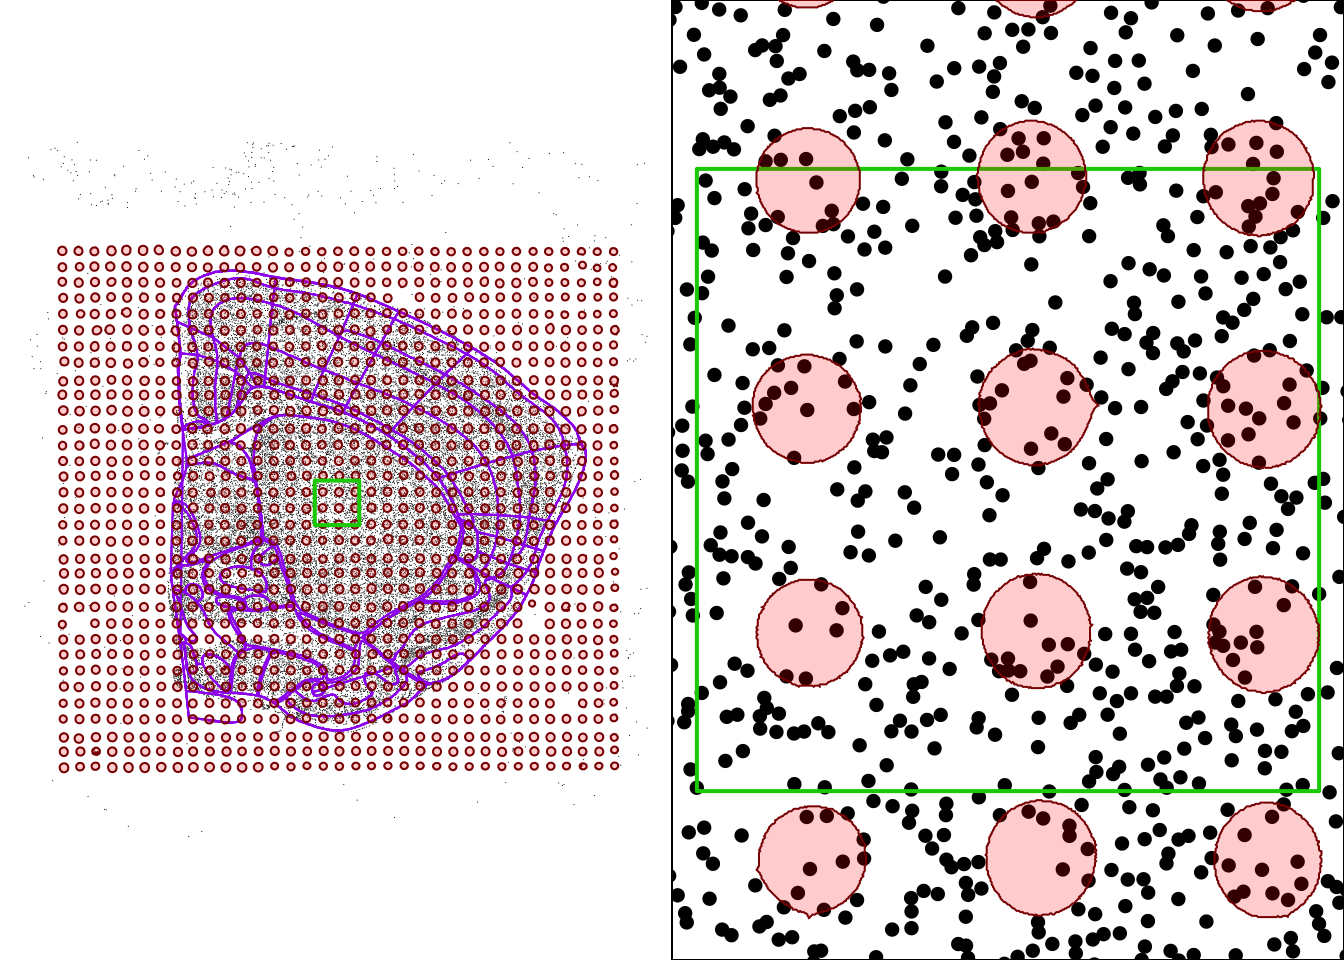
\includegraphics{wholebrain-bookdown_files/figure-latex/unnamed-chunk-4-1.pdf}

Then load in the integrated ST-data and WholeBrain dataset as a list
object called dataset with the following members:

\begin{itemize}
\tightlist
\item
  \texttt{dataset\$spots} data.frame object from
  \texttt{get.cells.ids(regi,\ seg.spots,\ forward.warps=TRUE)}
\item
  \texttt{dataset\$genes} data.frame object with transcript count where
  each row corresponds to the same row (spot) in \texttt{dataset\$spots}
  and each column is a gene.
\item
  \texttt{dataset\$nuclei} data.frame object from
  \texttt{get.cells.ids(regi,\ cells,\ forward.warps=TRUE)} contains all
  nuclei as rows and each nuclei is assigned to a spot.id
  (\texttt{datset\$nuclei\$spot.id}) corresponding to spot.id in
  \texttt{dataset\$spots\$spot.id}
\end{itemize}

\begin{Shaded}
\begin{Highlighting}[]
\CommentTok{#load combined ST-data and WholeBrain output as a list object called dataset with members }
\CommentTok{# dataset$spots (row= individual spots, col= region acronyms etc), dataset$genes (row = spots, col=genes)}
\CommentTok{# dataset$nuclei individually segmented nuclei with parent spot indicted by spot.id }
\CommentTok{# which have corresponding vector in dataset$spots$spot.id.}
\KeywordTok{load}\NormalTok{(}\StringTok{'./data/spatial_transcriptomics/170605/D2_S4_p1_0_mapped.RData'}\NormalTok{)}
\end{Highlighting}
\end{Shaded}

Your working space should now look like:

\begin{Shaded}
\begin{Highlighting}[]
\KeywordTok{ls}\NormalTok{()}
\end{Highlighting}
\end{Shaded}

\begin{verbatim}
## [1] "cells"         "dataset"       "polygon.atlas" "polygon.spot" 
## [5] "regi"          "roi"           "seg.spots"
\end{verbatim}

We can for example see that there is a good correlation between number
of nuclei inside a spot and number of detected genes:

\begin{Shaded}
\begin{Highlighting}[]
\NormalTok{genecount<-}\KeywordTok{apply}\NormalTok{(dataset$genes, }\DecValTok{1}\NormalTok{, function(x)}\KeywordTok{sum}\NormalTok{(x>}\DecValTok{0}\NormalTok{))}
\NormalTok{gene.expression<-}\KeywordTok{apply}\NormalTok{(dataset$genes, }\DecValTok{1}\NormalTok{, function(x)}\KeywordTok{mean}\NormalTok{(x[x>}\DecValTok{0}\NormalTok{]))}

\CommentTok{#Place Pearson correlation coefficient in quadrant.}
\NormalTok{get.quadrant<-function(x,y, }\DataTypeTok{lim=}\KeywordTok{c}\NormalTok{(}\FloatTok{0.75}\NormalTok{,}\FloatTok{0.85}\NormalTok{),}\DataTypeTok{col=}\StringTok{'black'}\NormalTok{)\{}
  \KeywordTok{text}\NormalTok{(}\KeywordTok{max}\NormalTok{(x, }\DataTypeTok{na.rm=}\OtherTok{TRUE}\NormalTok{)*lim[}\DecValTok{1}\NormalTok{],}
  \KeywordTok{max}\NormalTok{(y, }\DataTypeTok{na.rm=}\OtherTok{TRUE}\NormalTok{)*lim[}\DecValTok{2}\NormalTok{],}
  \KeywordTok{paste}\NormalTok{(}\StringTok{'R = '}\NormalTok{, }\KeywordTok{round}\NormalTok{(}\KeywordTok{cor}\NormalTok{(}\KeywordTok{na.omit}\NormalTok{(}\KeywordTok{cbind}\NormalTok{(x, y)))[}\DecValTok{1}\NormalTok{,}\DecValTok{2}\NormalTok{],}\DecValTok{2}\NormalTok{)),}
  \DataTypeTok{col=}\NormalTok{col}
  \NormalTok{)}
\NormalTok{\}}

\CommentTok{#plot}
\KeywordTok{par}\NormalTok{(}\DataTypeTok{mfrow=}\KeywordTok{c}\NormalTok{(}\DecValTok{1}\NormalTok{,}\DecValTok{2}\NormalTok{))}
\KeywordTok{par}\NormalTok{(}\DataTypeTok{yaxs=}\StringTok{'i'}\NormalTok{, }\DataTypeTok{xaxs=}\StringTok{'r'}\NormalTok{, }\DataTypeTok{mar=}\KeywordTok{c}\NormalTok{(}\DecValTok{2}\NormalTok{,}\DecValTok{4}\NormalTok{,}\DecValTok{1}\NormalTok{,}\DecValTok{2}\NormalTok{), }\DataTypeTok{mfrow=}\KeywordTok{c}\NormalTok{(}\DecValTok{2}\NormalTok{,}\DecValTok{1}\NormalTok{))}
\KeywordTok{plot}\NormalTok{(dataset$spots$nuclei, genecount, }\DataTypeTok{pch=}\DecValTok{16}\NormalTok{, }\DataTypeTok{cex=}\FloatTok{0.8}\NormalTok{, }\DataTypeTok{xlab=}\StringTok{'nuclei in spot'}\NormalTok{, }\DataTypeTok{ylab=}\StringTok{'Genes detected'}\NormalTok{, }\DataTypeTok{xlim=}\KeywordTok{c}\NormalTok{(}\DecValTok{0}\NormalTok{,}\DecValTok{50}\NormalTok{), }\DataTypeTok{ylim=}\KeywordTok{c}\NormalTok{(}\DecValTok{0}\NormalTok{,}\DecValTok{10000}\NormalTok{), }\DataTypeTok{axes=}\OtherTok{FALSE}\NormalTok{)}
\KeywordTok{get.quadrant}\NormalTok{(dataset$spots$nuclei, genecount, }\DataTypeTok{lim=}\KeywordTok{c}\NormalTok{(}\FloatTok{0.99}\NormalTok{,}\FloatTok{0.25}\NormalTok{))}
\KeywordTok{points}\NormalTok{(}\KeywordTok{data.frame}\NormalTok{(dataset$spots$nuclei, genecount)[}\KeywordTok{which}\NormalTok{(dataset$spots$spot.id%in%}\KeywordTok{c}\NormalTok{(}\DecValTok{693}\NormalTok{,}\DecValTok{706}\NormalTok{)),], }\DataTypeTok{pch=}\DecValTok{21}\NormalTok{, }\DataTypeTok{bg=}\KeywordTok{c}\NormalTok{(}\StringTok{'#998ec3'}\NormalTok{,}\StringTok{'#f1a340'}\NormalTok{), }\DataTypeTok{col=}\KeywordTok{c}\NormalTok{(}\StringTok{'#542788'}\NormalTok{, }\StringTok{'#b35806'}\NormalTok{), }\DataTypeTok{cex=}\FloatTok{1.2}\NormalTok{, }\DataTypeTok{lwd=}\FloatTok{1.5}\NormalTok{)}
\KeywordTok{axis}\NormalTok{(}\DecValTok{1}\NormalTok{, }\DataTypeTok{at=}\KeywordTok{c}\NormalTok{(}\DecValTok{0}\NormalTok{,}\DecValTok{25}\NormalTok{,}\DecValTok{50}\NormalTok{)) }
\KeywordTok{axis}\NormalTok{(}\DecValTok{2}\NormalTok{, }\DataTypeTok{at=}\KeywordTok{c}\NormalTok{(}\DecValTok{0}\NormalTok{,}\DecValTok{5000}\NormalTok{,}\DecValTok{10000}\NormalTok{), }\DataTypeTok{las=}\DecValTok{1}\NormalTok{)}
\KeywordTok{par}\NormalTok{(}\DataTypeTok{mar=}\KeywordTok{c}\NormalTok{(}\DecValTok{4}\NormalTok{,}\DecValTok{4}\NormalTok{,}\DecValTok{1}\NormalTok{,}\DecValTok{2}\NormalTok{))}
\KeywordTok{plot}\NormalTok{(dataset$spots$nuclei, gene.expression, }\DataTypeTok{pch=}\DecValTok{16}\NormalTok{, }\DataTypeTok{cex=}\FloatTok{0.8}\NormalTok{, }\DataTypeTok{xlab=}\StringTok{'nuclei in spot'}\NormalTok{, }\DataTypeTok{ylab=}\StringTok{'Avg. molecules }\CharTok{\textbackslash{}n}\StringTok{ per gene'}\NormalTok{, }\DataTypeTok{xlim=}\KeywordTok{c}\NormalTok{(}\DecValTok{0}\NormalTok{,}\DecValTok{50}\NormalTok{), }\DataTypeTok{ylim=}\KeywordTok{c}\NormalTok{(}\DecValTok{1}\NormalTok{,}\DecValTok{4}\NormalTok{), }\DataTypeTok{axes=}\OtherTok{FALSE}\NormalTok{)}
\KeywordTok{get.quadrant}\NormalTok{(dataset$spots$nuclei, gene.expression, }\DataTypeTok{lim=}\KeywordTok{c}\NormalTok{(}\FloatTok{0.95}\NormalTok{,}\FloatTok{0.35}\NormalTok{))}
\KeywordTok{points}\NormalTok{(}\KeywordTok{data.frame}\NormalTok{(dataset$spots$nuclei, gene.expression)[}\KeywordTok{which}\NormalTok{(dataset$spots$spot.id%in%}\KeywordTok{c}\NormalTok{(}\DecValTok{693}\NormalTok{,}\DecValTok{706}\NormalTok{)),], }\DataTypeTok{pch=}\DecValTok{21}\NormalTok{, }\DataTypeTok{bg=}\KeywordTok{c}\NormalTok{(}\StringTok{'#998ec3'}\NormalTok{,}\StringTok{'#f1a340'}\NormalTok{), }\DataTypeTok{col=}\KeywordTok{c}\NormalTok{(}\StringTok{'#542788'}\NormalTok{, }\StringTok{'#b35806'}\NormalTok{), }\DataTypeTok{cex=}\FloatTok{1.2}\NormalTok{, }\DataTypeTok{lwd=}\FloatTok{1.5}\NormalTok{)}
\KeywordTok{axis}\NormalTok{(}\DecValTok{1}\NormalTok{, }\DataTypeTok{at=}\KeywordTok{c}\NormalTok{(}\DecValTok{0}\NormalTok{,}\DecValTok{25}\NormalTok{,}\DecValTok{50}\NormalTok{)) }
\KeywordTok{axis}\NormalTok{(}\DecValTok{2}\NormalTok{, }\DataTypeTok{at=}\KeywordTok{c}\NormalTok{(}\DecValTok{1}\NormalTok{,}\FloatTok{2.5}\NormalTok{,}\DecValTok{4}\NormalTok{), }\DataTypeTok{las=}\DecValTok{1}\NormalTok{)}
\end{Highlighting}
\end{Shaded}

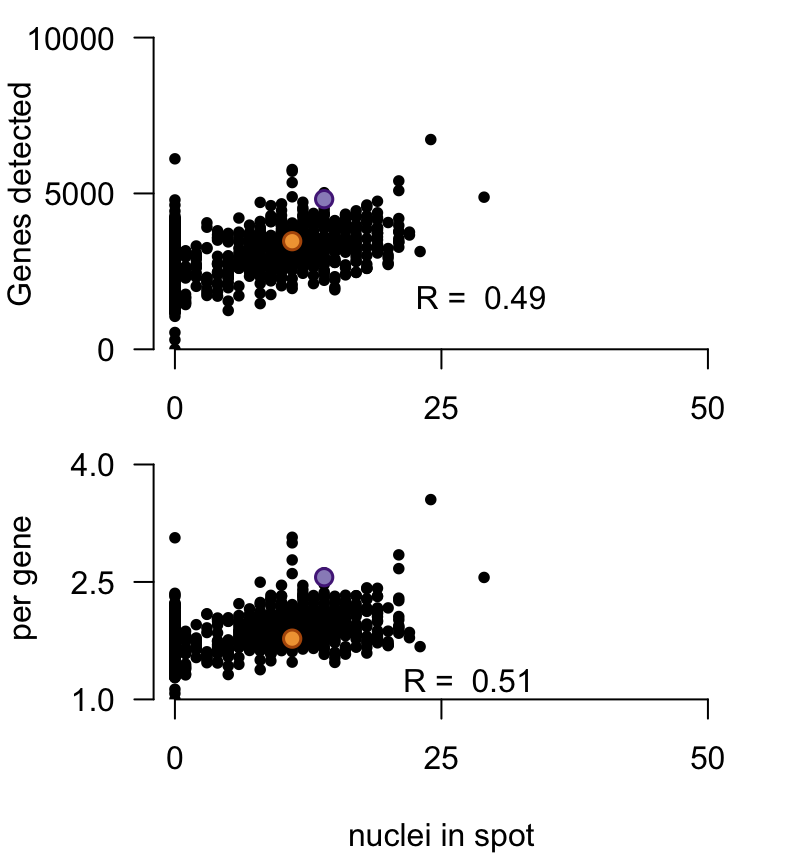
\includegraphics{wholebrain-bookdown_files/figure-latex/unnamed-chunk-7-1.pdf}

Let us now load in a custom plotting function for plotting gene
expression for individual genes using \texttt{base\ R}.

\section{Plotting gene expressions}\label{plotting-gene-expressions}

The function to display gene expression with base R is the following
load it into working space by running this code chunk:

\begin{Shaded}
\begin{Highlighting}[]
\NormalTok{plot.atlas<-function(regi, }\DataTypeTok{main=}\StringTok{''}\NormalTok{, }\DataTypeTok{xlim=}\KeywordTok{c}\NormalTok{(}\DecValTok{0}\NormalTok{,}\DecValTok{4}\NormalTok{), }\DataTypeTok{ylim=}\KeywordTok{c}\NormalTok{(-}\DecValTok{7}\NormalTok{, -}\DecValTok{1}\NormalTok{))\{}
  \NormalTok{scale.factor<-}\KeywordTok{mean}\NormalTok{(}\KeywordTok{c}\NormalTok{(regi$transformationgrid$height,regi$transformationgrid$width)/}\KeywordTok{dim}\NormalTok{(regi$transformationgrid$mx))}
  \NormalTok{regi<-}\KeywordTok{get.forward.warpRCPP}\NormalTok{(regi)}
  \NormalTok{region<-regi$atlas$outlines[[}\DecValTok{1}\NormalTok{]][}\KeywordTok{c}\NormalTok{(}\DecValTok{2}\NormalTok{*}\DecValTok{1-1}\NormalTok{,}\DecValTok{2}\NormalTok{*}\DecValTok{1}\NormalTok{)]}
      \KeywordTok{names}\NormalTok{(region)<-}\KeywordTok{c}\NormalTok{(}\StringTok{'x'}\NormalTok{, }\StringTok{'y'}\NormalTok{)}
      \NormalTok{index<-}\KeywordTok{round}\NormalTok{(}\KeywordTok{cbind}\NormalTok{(region$y, region$x))*scale.factor}
      \CommentTok{#region$x<-regi$transformationgrid$mxF[index]}
      \CommentTok{#region$y<-regi$transformationgrid$myF[index]}
      \NormalTok{region<-}\KeywordTok{list}\NormalTok{(}\DataTypeTok{x=}\NormalTok{index[,}\DecValTok{2}\NormalTok{], }\DataTypeTok{y=}\NormalTok{index[,}\DecValTok{1}\NormalTok{])}
      \NormalTok{region<-}\KeywordTok{stereotactic.coordinates}\NormalTok{(region$x, region$y, regi, }\DataTypeTok{inverse=}\OtherTok{FALSE}\NormalTok{)}
      \KeywordTok{plot}\NormalTok{(region, }\DataTypeTok{asp=}\DecValTok{1}\NormalTok{, }\DataTypeTok{type=}\StringTok{'n'}\NormalTok{, }\DataTypeTok{axes=}\OtherTok{FALSE}\NormalTok{, }\DataTypeTok{main =} \NormalTok{main, }\DataTypeTok{ylab=}\StringTok{'Dorso-ventral (mm)'}\NormalTok{, }\DataTypeTok{xlab=}\StringTok{'Medio-lateral (mm)'}\NormalTok{)}
  
  \NormalTok{for(j in }\DecValTok{1}\NormalTok{:regi$atlas$numRegions)\{ }
    \NormalTok{for(i in }\DecValTok{1}\NormalTok{:}\DecValTok{2}\NormalTok{)\{}
      \NormalTok{region<-regi$atlas$outlines[[j]][}\KeywordTok{c}\NormalTok{(}\DecValTok{2}\NormalTok{*}\DecValTok{1-1}\NormalTok{,}\DecValTok{2}\NormalTok{*}\DecValTok{1}\NormalTok{)]}
      \KeywordTok{names}\NormalTok{(region)<-}\KeywordTok{c}\NormalTok{(}\StringTok{'x'}\NormalTok{, }\StringTok{'y'}\NormalTok{)}
      \NormalTok{index<-}\KeywordTok{round}\NormalTok{(}\KeywordTok{cbind}\NormalTok{(region$y, region$x))*scale.factor}
      \CommentTok{#region$x<-regi$transformationgrid$mxF[index]}
      \CommentTok{#region$y<-regi$transformationgrid$myF[index]}
      \NormalTok{region<-}\KeywordTok{list}\NormalTok{(}\DataTypeTok{x=}\NormalTok{index[,}\DecValTok{2}\NormalTok{], }\DataTypeTok{y=}\NormalTok{index[,}\DecValTok{1}\NormalTok{])}
      \NormalTok{region<-}\KeywordTok{stereotactic.coordinates}\NormalTok{(region$x, region$y, regi, }\DataTypeTok{inverse=}\OtherTok{FALSE}\NormalTok{)}
      \KeywordTok{polygon}\NormalTok{(region$x, region$y, }\DataTypeTok{border=}\StringTok{'black'}\NormalTok{, }\DataTypeTok{col=}\KeywordTok{gray}\NormalTok{(}\FloatTok{0.95}\NormalTok{))}
    \NormalTok{\}}
  \NormalTok{\}}
  \NormalTok{xlim<-}\KeywordTok{sort}\NormalTok{(xlim, }\DataTypeTok{decreasing=}\OtherTok{TRUE}\NormalTok{)}
  \NormalTok{ylim<-}\KeywordTok{sort}\NormalTok{(ylim, }\DataTypeTok{decreasing=}\OtherTok{TRUE}\NormalTok{)}
  
  \KeywordTok{axis}\NormalTok{(}\DecValTok{2}\NormalTok{, }\DataTypeTok{at =} \KeywordTok{seq}\NormalTok{(ylim[}\DecValTok{1}\NormalTok{], ylim[}\DecValTok{2}\NormalTok{],}\DataTypeTok{by=}\NormalTok{-}\FloatTok{0.1}\NormalTok{), }\DataTypeTok{labels =} \OtherTok{FALSE}\NormalTok{, }\DataTypeTok{las =} \DecValTok{1}\NormalTok{, }\DataTypeTok{col =} \StringTok{"orange"}\NormalTok{, }\DataTypeTok{tck =} \NormalTok{-}\FloatTok{0.0125}\NormalTok{)}
  \KeywordTok{axis}\NormalTok{(}\DecValTok{2}\NormalTok{, }\DataTypeTok{at =} \KeywordTok{seq}\NormalTok{(ylim[}\DecValTok{1}\NormalTok{], ylim[}\DecValTok{2}\NormalTok{], }\DataTypeTok{by=}\NormalTok{-}\FloatTok{0.5}\NormalTok{), }\DataTypeTok{labels =} \OtherTok{FALSE}\NormalTok{, }\DataTypeTok{las =} \DecValTok{1}\NormalTok{, }\DataTypeTok{col =} \StringTok{"darkblue"}\NormalTok{, }\DataTypeTok{tck =} \NormalTok{-}\FloatTok{0.025}\NormalTok{)}
  \KeywordTok{axis}\NormalTok{(}\DecValTok{2}\NormalTok{, }\DataTypeTok{at =} \NormalTok{ylim[}\DecValTok{1}\NormalTok{]:ylim[}\DecValTok{2}\NormalTok{],  }\DataTypeTok{las =} \DecValTok{1}\NormalTok{)                }
  
  \KeywordTok{axis}\NormalTok{(}\DecValTok{1}\NormalTok{, }\DataTypeTok{at =} \KeywordTok{seq}\NormalTok{(xlim[}\DecValTok{1}\NormalTok{], -xlim[}\DecValTok{2}\NormalTok{],}\DataTypeTok{by=}\NormalTok{-}\FloatTok{0.1}\NormalTok{), }\DataTypeTok{labels =} \OtherTok{FALSE}\NormalTok{, }\DataTypeTok{las =} \DecValTok{1}\NormalTok{, }\DataTypeTok{col =} \StringTok{"orange"}\NormalTok{, }\DataTypeTok{tck =} \NormalTok{-}\FloatTok{0.0125}\NormalTok{)}
  \KeywordTok{axis}\NormalTok{(}\DecValTok{1}\NormalTok{, }\DataTypeTok{at =} \KeywordTok{seq}\NormalTok{(xlim[}\DecValTok{1}\NormalTok{], -xlim[}\DecValTok{2}\NormalTok{], }\DataTypeTok{by=}\NormalTok{-}\FloatTok{0.5}\NormalTok{), }\DataTypeTok{labels =} \OtherTok{FALSE}\NormalTok{, }\DataTypeTok{las =} \DecValTok{1}\NormalTok{, }\DataTypeTok{col =} \StringTok{"darkblue"}\NormalTok{, }\DataTypeTok{tck =} \NormalTok{-}\FloatTok{0.025}\NormalTok{)}
  \KeywordTok{axis}\NormalTok{(}\DecValTok{1}\NormalTok{, }\DataTypeTok{at =} \NormalTok{xlim[}\DecValTok{1}\NormalTok{]:xlim[}\DecValTok{2}\NormalTok{],  }\DataTypeTok{las =} \DecValTok{1}\NormalTok{)                  }
   
\NormalTok{\}}

\NormalTok{plot.gene<-function(dataset, regi, gene, }\DataTypeTok{colorfunc =} \NormalTok{heat.colors, }\DataTypeTok{atlas=}\OtherTok{TRUE}\NormalTok{)\{}
  \NormalTok{if(atlas)}
    \KeywordTok{plot.atlas}\NormalTok{(regi, }\DataTypeTok{main=}\NormalTok{gene)}

  \NormalTok{gene<-dataset$genes[,gene]}
  \NormalTok{colors <-}\StringTok{ }\KeywordTok{mapply}\NormalTok{(function(col, i) }\KeywordTok{adjustcolor}\NormalTok{(col, }\DataTypeTok{alpha.f =} \NormalTok{(gene/}\KeywordTok{max}\NormalTok{(gene))[i]), }
                 \KeywordTok{colorfunc}\NormalTok{(}\KeywordTok{length}\NormalTok{(}\KeywordTok{unique}\NormalTok{(gene)))[gene}\DecValTok{+1}\NormalTok{], }\KeywordTok{seq_along}\NormalTok{(gene))   }

  \NormalTok{inside.tissue<-!}\KeywordTok{is.na}\NormalTok{(dataset$spots$acronym)}
  \KeywordTok{points}\NormalTok{(dataset$spots$ML[inside.tissue], dataset$spots$DV[inside.tissue], }\DataTypeTok{pch=}\DecValTok{16}\NormalTok{, }\DataTypeTok{col=}\NormalTok{colors[inside.tissue])}
\NormalTok{\} }

\NormalTok{legend.gene<-function(dataset, gene, }\DataTypeTok{colorfunc =} \NormalTok{heat.colors)\{}
  \KeywordTok{par}\NormalTok{(}\DataTypeTok{xaxs=}\StringTok{'i'}\NormalTok{)}
  \KeywordTok{plot}\NormalTok{(}\KeywordTok{c}\NormalTok{(}\DecValTok{0}\NormalTok{,}\DecValTok{1}\NormalTok{),}\KeywordTok{c}\NormalTok{(}\DecValTok{0}\NormalTok{,}\DecValTok{1}\NormalTok{),}\DataTypeTok{type =} \StringTok{'n'}\NormalTok{, }\DataTypeTok{axes =} \NormalTok{F,}\DataTypeTok{xlab =} \StringTok{''}\NormalTok{, }\DataTypeTok{ylab =} \StringTok{''}\NormalTok{, }\DataTypeTok{main =} \NormalTok{gene, }\DataTypeTok{xlim=}\KeywordTok{c}\NormalTok{(}\DecValTok{0}\NormalTok{,}\DecValTok{1}\NormalTok{))}
  \NormalTok{gene<-dataset$genes[,gene]}
  \NormalTok{color<-}\KeywordTok{sapply}\NormalTok{(}\KeywordTok{seq_along}\NormalTok{(}\KeywordTok{unique}\NormalTok{(gene)), function(x)\{}\KeywordTok{adjustcolor}\NormalTok{(}\KeywordTok{colorfunc}\NormalTok{(}\KeywordTok{length}\NormalTok{(}\KeywordTok{unique}\NormalTok{(gene)))[x], }\DataTypeTok{alpha.f =} \NormalTok{(}\KeywordTok{sort}\NormalTok{(}\KeywordTok{unique}\NormalTok{(gene))/}\KeywordTok{max}\NormalTok{(gene))[x] )\} )}
  \NormalTok{legend_image <-}\StringTok{ }\KeywordTok{as.raster}\NormalTok{(}\KeywordTok{matrix}\NormalTok{(}\KeywordTok{rev}\NormalTok{(color), }\DataTypeTok{ncol=}\DecValTok{1}\NormalTok{))}
  \KeywordTok{axis}\NormalTok{(}\DecValTok{4}\NormalTok{, }\DataTypeTok{at =} \KeywordTok{seq}\NormalTok{(}\DecValTok{0}\NormalTok{,}\DecValTok{1}\NormalTok{,}\DataTypeTok{l=}\DecValTok{5}\NormalTok{), }\DataTypeTok{labels =} \KeywordTok{seq}\NormalTok{(}\DecValTok{0}\NormalTok{,}\KeywordTok{max}\NormalTok{(gene),}\DataTypeTok{l=}\DecValTok{5}\NormalTok{), }\DataTypeTok{las=}\DecValTok{1}\NormalTok{)}
  \KeywordTok{rasterImage}\NormalTok{(legend_image, }\DecValTok{0}\NormalTok{, }\DecValTok{0}\NormalTok{, }\DecValTok{1}\NormalTok{,}\DecValTok{1}\NormalTok{)}
  \KeywordTok{polygon}\NormalTok{(}\KeywordTok{c}\NormalTok{(}\DecValTok{0}\NormalTok{,}\DecValTok{1}\NormalTok{,}\DecValTok{1}\NormalTok{,}\DecValTok{0}\NormalTok{), }\KeywordTok{c}\NormalTok{(}\DecValTok{0}\NormalTok{, }\DecValTok{0}\NormalTok{, }\DecValTok{1}\NormalTok{,}\DecValTok{1}\NormalTok{))}
  \KeywordTok{mtext}\NormalTok{(}\StringTok{'Count'}\NormalTok{,}\DecValTok{4}\NormalTok{,}\FloatTok{3.5}\NormalTok{)}
  \NormalTok{histogram<-}\KeywordTok{hist}\NormalTok{(gene, }\DataTypeTok{breaks=}\KeywordTok{seq}\NormalTok{(}\DecValTok{0}\NormalTok{,}\KeywordTok{max}\NormalTok{(gene)), }\DataTypeTok{plot=}\OtherTok{FALSE}\NormalTok{)}
  \NormalTok{y<-histogram$counts}
  \NormalTok{y<-}\KeywordTok{log2}\NormalTok{(y}\DecValTok{+1}\NormalTok{)}
  \NormalTok{y<-}\FloatTok{0.5}\NormalTok{*(y/}\KeywordTok{max}\NormalTok{(y))}
  \NormalTok{x<-(histogram$mids}\FloatTok{-0.5}\NormalTok{)/}\KeywordTok{max}\NormalTok{(histogram$mids}\FloatTok{-0.5}\NormalTok{)}
  \NormalTok{y<-}\KeywordTok{c}\NormalTok{(}\DecValTok{0}\NormalTok{, -}\KeywordTok{rep}\NormalTok{(y, }\DataTypeTok{each=}\DecValTok{2}\NormalTok{)[-}\KeywordTok{length}\NormalTok{(}\KeywordTok{rep}\NormalTok{(y, }\DataTypeTok{each=}\DecValTok{2}\NormalTok{))])}
  \NormalTok{x<-}\KeywordTok{rep}\NormalTok{(x, }\DataTypeTok{each=}\DecValTok{2}\NormalTok{)}
  \KeywordTok{par}\NormalTok{(}\DataTypeTok{xpd=}\NormalTok{T)}
  \KeywordTok{polygon}\NormalTok{(}\KeywordTok{c}\NormalTok{(y, }\KeywordTok{rep}\NormalTok{(}\DecValTok{0}\NormalTok{, }\KeywordTok{length}\NormalTok{(y))), }\KeywordTok{c}\NormalTok{(x, }\KeywordTok{rev}\NormalTok{(x)), }\DataTypeTok{col=}\StringTok{'purple'}\NormalTok{)}
  \KeywordTok{par}\NormalTok{(}\DataTypeTok{xpd=}\NormalTok{F)}
\NormalTok{\}}
\end{Highlighting}
\end{Shaded}

\begin{Shaded}
\begin{Highlighting}[]
\CommentTok{#viridis for color scale}
\KeywordTok{library}\NormalTok{(viridis)}
\end{Highlighting}
\end{Shaded}

Now we can plot any gene like this:

\begin{Shaded}
\begin{Highlighting}[]
\KeywordTok{layout}\NormalTok{(}\KeywordTok{matrix}\NormalTok{(}\DecValTok{1}\NormalTok{:}\DecValTok{2}\NormalTok{,}\DataTypeTok{ncol=}\DecValTok{2}\NormalTok{), }\DataTypeTok{width =} \KeywordTok{c}\NormalTok{(}\DecValTok{4}\NormalTok{,}\DecValTok{3}\NormalTok{),}\DataTypeTok{height =} \KeywordTok{c}\NormalTok{(}\DecValTok{1}\NormalTok{,}\DecValTok{1}\NormalTok{))}
\KeywordTok{par}\NormalTok{(}\DataTypeTok{mar=}\KeywordTok{c}\NormalTok{(}\DecValTok{4}\NormalTok{,}\DecValTok{4}\NormalTok{,}\DecValTok{4}\NormalTok{,}\DecValTok{0}\NormalTok{))}
\KeywordTok{plot.gene}\NormalTok{(dataset, regi, }\DataTypeTok{gene=}\StringTok{'Penk'}\NormalTok{, }\DataTypeTok{colorfunc=}\NormalTok{viridis)}
\KeywordTok{par}\NormalTok{(}\DataTypeTok{mar=}\KeywordTok{c}\NormalTok{(}\DecValTok{4}\NormalTok{,}\DecValTok{2}\NormalTok{,}\DecValTok{4}\NormalTok{,}\DecValTok{10}\NormalTok{))}
\KeywordTok{legend.gene}\NormalTok{(dataset, }\DataTypeTok{gene=}\StringTok{'Penk'}\NormalTok{, }\DataTypeTok{colorfunc=}\NormalTok{viridis)}
\end{Highlighting}
\end{Shaded}

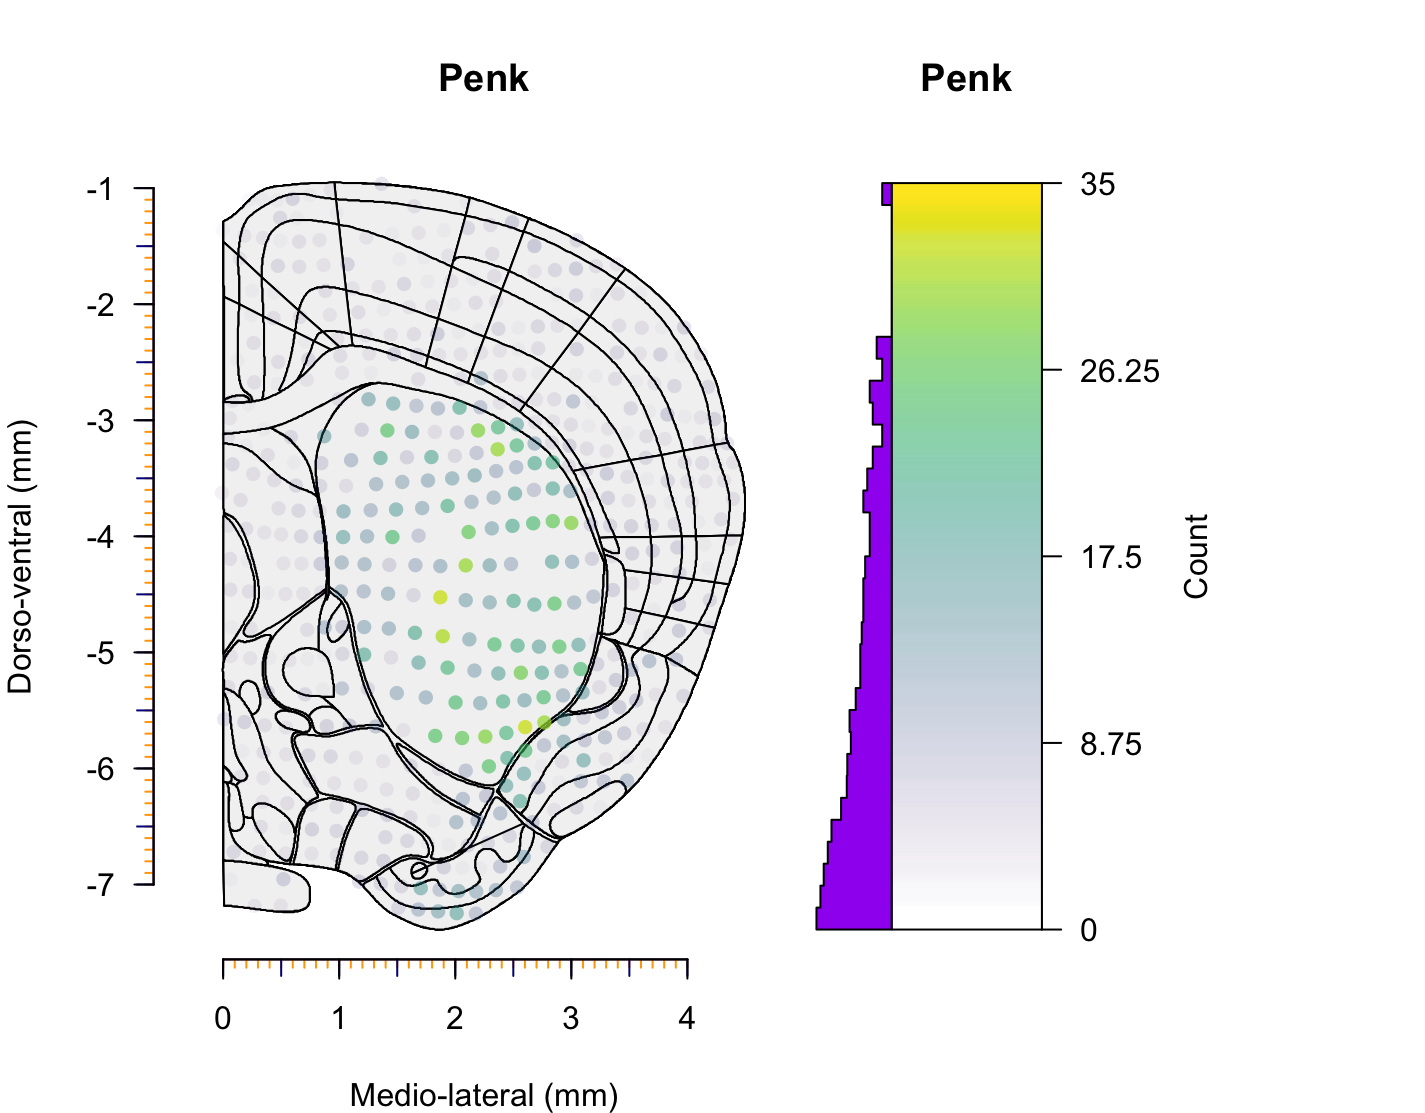
\includegraphics{wholebrain-bookdown_files/figure-latex/unnamed-chunk-11-1.pdf}

Now lets declare a plotting function for plotting all genes we throw at
it in a vector:

\begin{Shaded}
\begin{Highlighting}[]
\NormalTok{plot.these.genes<-function(genelist)\{}
\NormalTok{non.detected<-}\KeywordTok{character}\NormalTok{()}
\NormalTok{striatum<-}\KeywordTok{character}\NormalTok{()}
\NormalTok{somatosensory<-}\KeywordTok{character}\NormalTok{()}
\NormalTok{for(i in genelist)\{}

\NormalTok{if(}\KeywordTok{sum}\NormalTok{(i%in%}\KeywordTok{names}\NormalTok{(dataset$genes)) )\{}
  \KeywordTok{layout}\NormalTok{(}\KeywordTok{matrix}\NormalTok{(}\DecValTok{1}\NormalTok{:}\DecValTok{2}\NormalTok{,}\DataTypeTok{ncol=}\DecValTok{2}\NormalTok{), }\DataTypeTok{width =} \KeywordTok{c}\NormalTok{(}\DecValTok{2}\NormalTok{,}\DecValTok{1}\NormalTok{),}\DataTypeTok{height =} \KeywordTok{c}\NormalTok{(}\DecValTok{1}\NormalTok{,}\DecValTok{1}\NormalTok{))}
  \KeywordTok{par}\NormalTok{(}\DataTypeTok{mar=}\KeywordTok{c}\NormalTok{(}\DecValTok{4}\NormalTok{,}\DecValTok{4}\NormalTok{,}\DecValTok{4}\NormalTok{,}\DecValTok{0}\NormalTok{))}
  \KeywordTok{plot.gene}\NormalTok{(dataset, regi, }\DataTypeTok{gene=}\NormalTok{i, }\DataTypeTok{colorfunc=}\NormalTok{viridis)}
  \KeywordTok{par}\NormalTok{(}\DataTypeTok{mar=}\KeywordTok{c}\NormalTok{(}\DecValTok{4}\NormalTok{,}\DecValTok{2}\NormalTok{,}\DecValTok{4}\NormalTok{,}\DecValTok{5}\NormalTok{))}
  \KeywordTok{legend.gene}\NormalTok{(dataset, }\DataTypeTok{gene=}\NormalTok{i, }\DataTypeTok{colorfunc=}\NormalTok{viridis)}
  
  \KeywordTok{cat}\NormalTok{(i)}
  \NormalTok{region.index<-}\KeywordTok{substr}\NormalTok{(dataset$spots$acronym, }\DecValTok{1}\NormalTok{,}\DecValTok{2}\NormalTok{)}
  \NormalTok{CP<-dataset$genes[}\KeywordTok{which}\NormalTok{(region.index==}\StringTok{'CP'}\NormalTok{), i]}
  \NormalTok{SS<-dataset$genes[}\KeywordTok{which}\NormalTok{(region.index==}\StringTok{'SS'}\NormalTok{), i]}
  \NormalTok{ttest<-}\KeywordTok{t.test}\NormalTok{(CP, SS)}
  \NormalTok{if(!}\KeywordTok{is.nan}\NormalTok{(ttest$p.value))\{}
    \NormalTok{if(ttest$p.value<}\FloatTok{0.05}\NormalTok{)\{}
      \KeywordTok{cat}\NormalTok{(}\StringTok{'        █▬█ █ ▀█▀'}\NormalTok{)}
      \NormalTok{if(ttest$statistic<}\DecValTok{0}\NormalTok{)\{}
        \KeywordTok{cat}\NormalTok{(}\StringTok{' MARKER FOR SOMATOSENSORY!'}\NormalTok{)}
        \NormalTok{somatosensory<-}\KeywordTok{append}\NormalTok{(somatosensory, i)}
      \NormalTok{\}else\{}
        \KeywordTok{cat}\NormalTok{(}\StringTok{' MARKER FOR CAUDATE PUTAMEN!'}\NormalTok{)}
        \NormalTok{striatum<-}\KeywordTok{append}\NormalTok{(striatum, i)}
      \NormalTok{\}}
    \NormalTok{\}}
  \NormalTok{\}}
 
  \KeywordTok{cat}\NormalTok{(}\KeywordTok{paste}\NormalTok{(}\StringTok{'}\CharTok{\textbackslash{}n}\StringTok{ -----}\CharTok{\textbackslash{}n}\StringTok{ Average number of'}\NormalTok{, i,}\StringTok{'transcripts detected:}\CharTok{\textbackslash{}n}\StringTok{ CPu : M ='}\NormalTok{, }\KeywordTok{round}\NormalTok{(}\KeywordTok{mean}\NormalTok{(CP), }\DecValTok{2}\NormalTok{), }\StringTok{'( SD ='}\NormalTok{, }\KeywordTok{round}\NormalTok{(}\KeywordTok{sd}\NormalTok{(CP), }\DecValTok{2}\NormalTok{),}\StringTok{')'}\NormalTok{, }\StringTok{'molecules }\CharTok{\textbackslash{}n}\StringTok{ SS : M ='}\NormalTok{, }\KeywordTok{round}\NormalTok{(}\KeywordTok{mean}\NormalTok{(SS), }\DecValTok{2}\NormalTok{)), }\StringTok{'( SD ='}\NormalTok{, }\KeywordTok{round}\NormalTok{(}\KeywordTok{sd}\NormalTok{(SS), }\DecValTok{2}\NormalTok{),}\StringTok{') molecules}\CharTok{\textbackslash{}n}\StringTok{ -----}\CharTok{\textbackslash{}n}\StringTok{'}\NormalTok{)}
  \KeywordTok{print}\NormalTok{(ttest)}
\NormalTok{\}else\{}
  \NormalTok{non.detected<-}\KeywordTok{append}\NormalTok{(non.detected, i)}
\NormalTok{\}}
\NormalTok{\}}
\KeywordTok{cat}\NormalTok{(}\KeywordTok{paste0}\NormalTok{(}\StringTok{'}\CharTok{\textbackslash{}n}\StringTok{ Nondetected genes: }\CharTok{\textbackslash{}n}\StringTok{'}\NormalTok{, }\KeywordTok{paste0}\NormalTok{(non.detected, }\DataTypeTok{collapse=}\StringTok{', '}\NormalTok{)))}
\KeywordTok{return}\NormalTok{(}\KeywordTok{list}\NormalTok{(}\DataTypeTok{non.detected =} \NormalTok{non.detected, }\DataTypeTok{striatum =} \NormalTok{striatum, }\DataTypeTok{somatosensory =} \NormalTok{somatosensory))}
\NormalTok{\}}
\end{Highlighting}
\end{Shaded}

\section{Confirmatory analysis}\label{confirmatory-analysis}

Running \texttt{plot.these.genes()} with a character vector of genes
that we are interested will plot all of them:

\begin{Shaded}
\begin{Highlighting}[]
\CommentTok{#Genes that are differentially expressed between striatal and somatosensory cortical astrocytes:}
\NormalTok{astrocytes<-}\KeywordTok{c}\NormalTok{(}\StringTok{"Crym"}\NormalTok{, }\StringTok{"6330403K07Rik"}\NormalTok{, }\StringTok{"Prss56"}\NormalTok{, }\StringTok{"Fam134b"}\NormalTok{, }\StringTok{"Sntb1"}\NormalTok{, }\StringTok{"Rcn1"}\NormalTok{, }\StringTok{"Nme6"}\NormalTok{, }\StringTok{"Bex2"}\NormalTok{, }\StringTok{"Hey2"}\NormalTok{, }\StringTok{"Sepn1"}\NormalTok{, }\StringTok{"Ints12"}\NormalTok{, }\StringTok{"Abtb2"}\NormalTok{, }\StringTok{"Olig2"}\NormalTok{,}\StringTok{"Vps18"}\NormalTok{,}\StringTok{"Ppif"}\NormalTok{, }\StringTok{"Gpd1"}\NormalTok{, }\StringTok{"Olig1"}\NormalTok{, }\StringTok{"Slc25a18"}\NormalTok{)}
\NormalTok{conf.analysis<-}\KeywordTok{plot.these.genes}\NormalTok{(astrocytes)}
\end{Highlighting}
\end{Shaded}

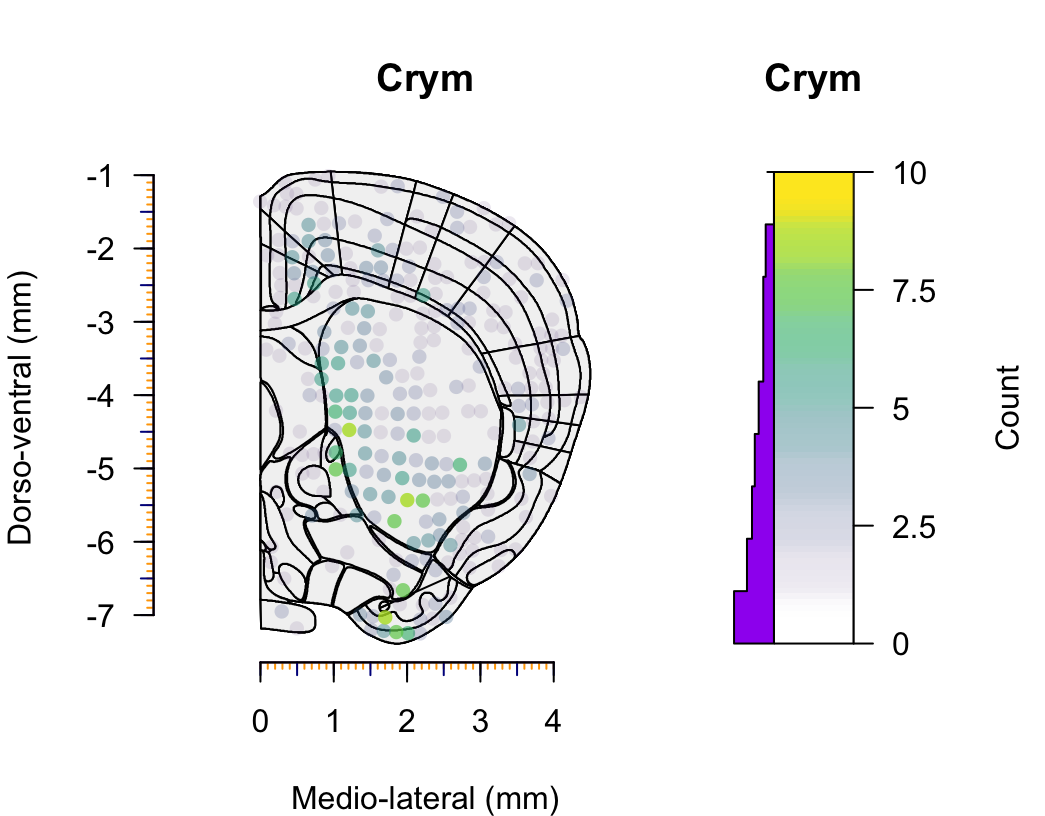
\includegraphics{wholebrain-bookdown_files/figure-latex/unnamed-chunk-13-1.pdf}

\begin{verbatim}
## Crym        █▬█ █ ▀█▀ MARKER FOR CAUDATE PUTAMEN!
##  -----
##  Average number of Crym transcripts detected:
##  CPu : M = 2.17 ( SD = 2.19 ) molecules 
##  SS : M = 0.63 ( SD = 0.8 ) molecules
##  -----
## 
##  Welch Two Sample t-test
## 
## data:  CP and SS
## t = 7.1829, df = 145.34, p-value = 3.274e-11
## alternative hypothesis: true difference in means is not equal to 0
## 95 percent confidence interval:
##  1.119830 1.970018
## sample estimates:
## mean of x mean of y 
## 2.1709402 0.6260163
\end{verbatim}

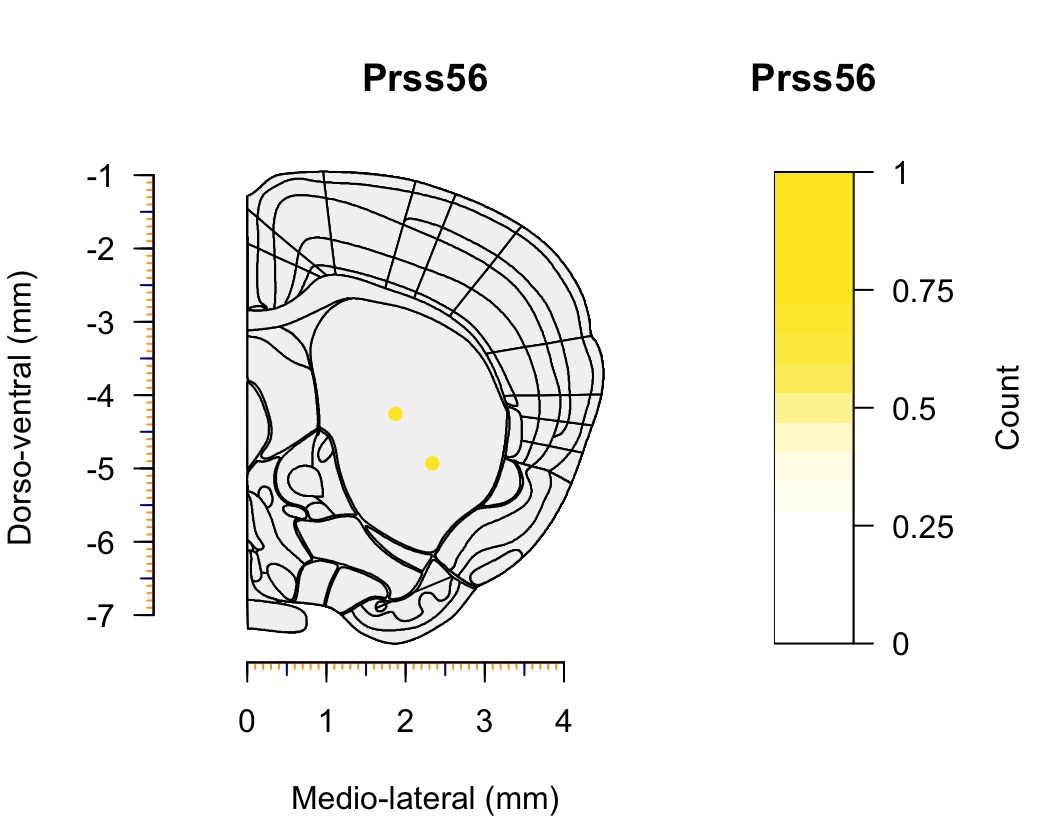
\includegraphics{wholebrain-bookdown_files/figure-latex/unnamed-chunk-13-2.pdf}

\begin{verbatim}
## Prss56
##  -----
##  Average number of Prss56 transcripts detected:
##  CPu : M = 0.02 ( SD = 0.13 ) molecules 
##  SS : M = 0 ( SD = 0 ) molecules
##  -----
## 
##  Welch Two Sample t-test
## 
## data:  CP and SS
## t = 1.4203, df = 116, p-value = 0.1582
## alternative hypothesis: true difference in means is not equal to 0
## 95 percent confidence interval:
##  -0.00674298  0.04093101
## sample estimates:
##  mean of x  mean of y 
## 0.01709402 0.00000000
\end{verbatim}

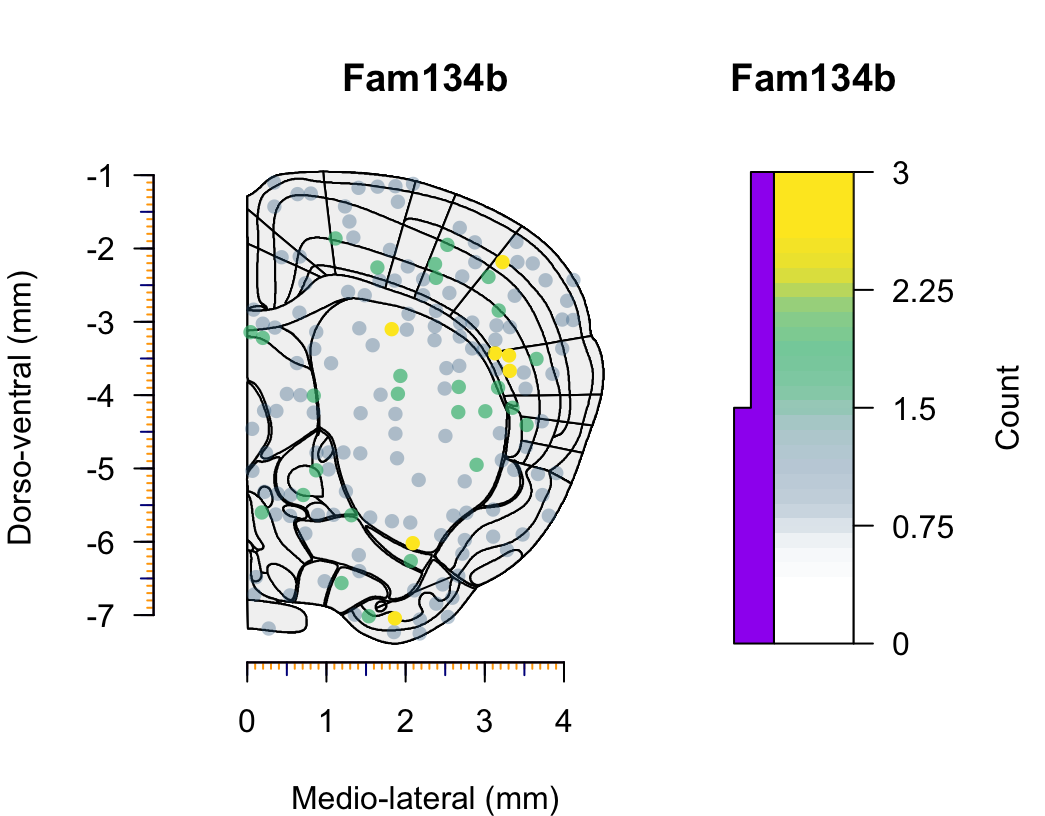
\includegraphics{wholebrain-bookdown_files/figure-latex/unnamed-chunk-13-3.pdf}

\begin{verbatim}
## Fam134b
##  -----
##  Average number of Fam134b transcripts detected:
##  CPu : M = 0.41 ( SD = 0.67 ) molecules 
##  SS : M = 0.42 ( SD = 0.74 ) molecules
##  -----
## 
##  Welch Two Sample t-test
## 
## data:  CP and SS
## t = -0.13768, df = 237.6, p-value = 0.8906
## alternative hypothesis: true difference in means is not equal to 0
## 95 percent confidence interval:
##  -0.1914788  0.1664632
## sample estimates:
## mean of x mean of y 
## 0.4102564 0.4227642
\end{verbatim}

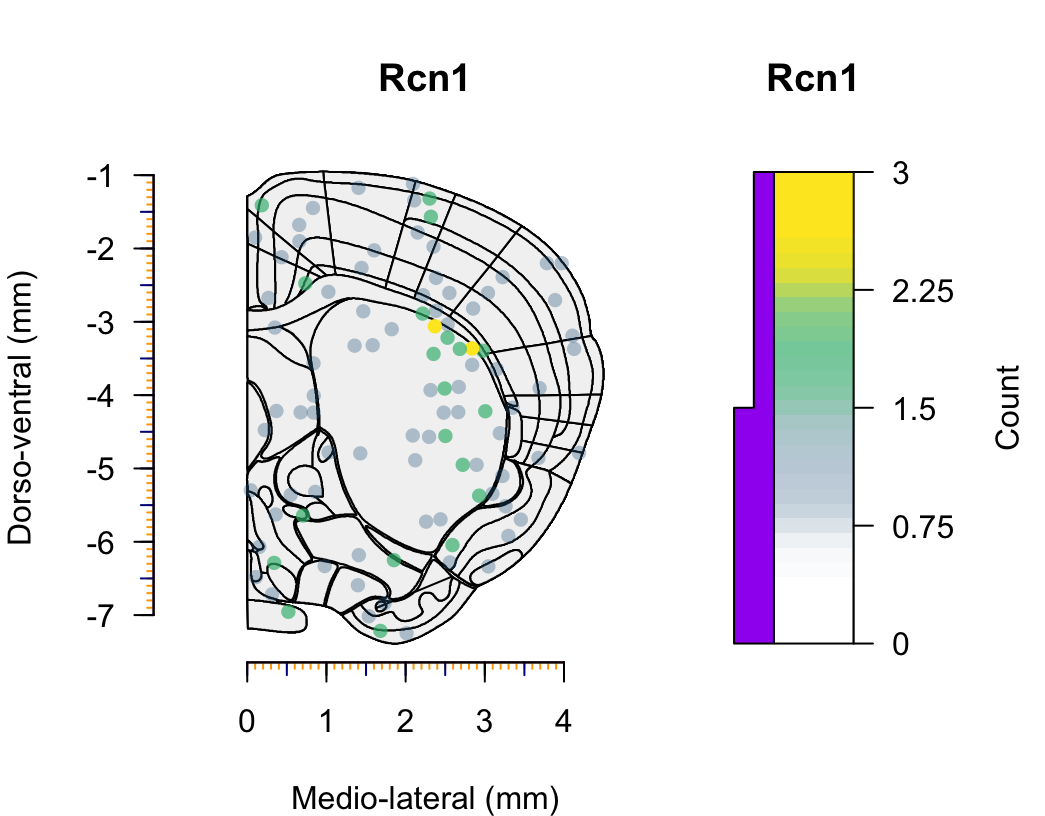
\includegraphics{wholebrain-bookdown_files/figure-latex/unnamed-chunk-13-4.pdf}

\begin{verbatim}
## Rcn1        █▬█ █ ▀█▀ MARKER FOR CAUDATE PUTAMEN!
##  -----
##  Average number of Rcn1 transcripts detected:
##  CPu : M = 0.34 ( SD = 0.68 ) molecules 
##  SS : M = 0.16 ( SD = 0.41 ) molecules
##  -----
## 
##  Welch Two Sample t-test
## 
## data:  CP and SS
## t = 2.443, df = 188.58, p-value = 0.01549
## alternative hypothesis: true difference in means is not equal to 0
## 95 percent confidence interval:
##  0.03451781 0.32403962
## sample estimates:
## mean of x mean of y 
## 0.3418803 0.1626016
\end{verbatim}

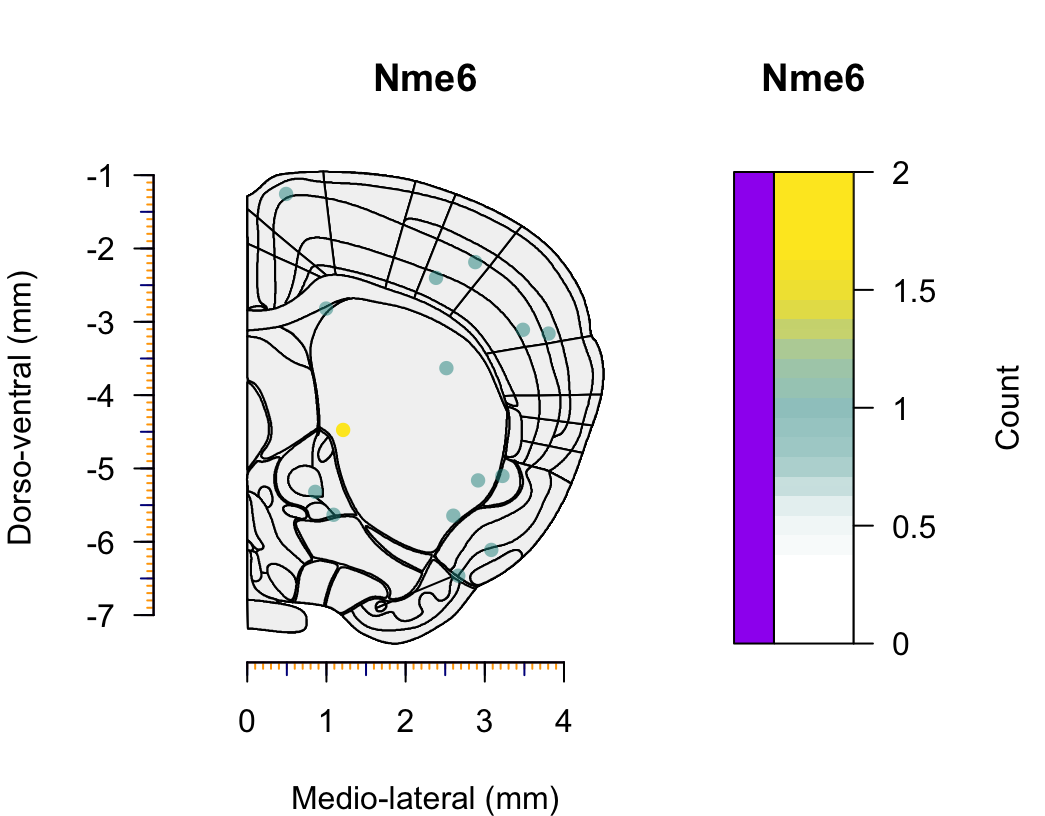
\includegraphics{wholebrain-bookdown_files/figure-latex/unnamed-chunk-13-5.pdf}

\begin{verbatim}
## Nme6
##  -----
##  Average number of Nme6 transcripts detected:
##  CPu : M = 0.04 ( SD = 0.24 ) molecules 
##  SS : M = 0.03 ( SD = 0.18 ) molecules
##  -----
## 
##  Welch Two Sample t-test
## 
## data:  CP and SS
## t = 0.37104, df = 212.71, p-value = 0.711
## alternative hypothesis: true difference in means is not equal to 0
## 95 percent confidence interval:
##  -0.04405236  0.06448180
## sample estimates:
##  mean of x  mean of y 
## 0.04273504 0.03252033
\end{verbatim}

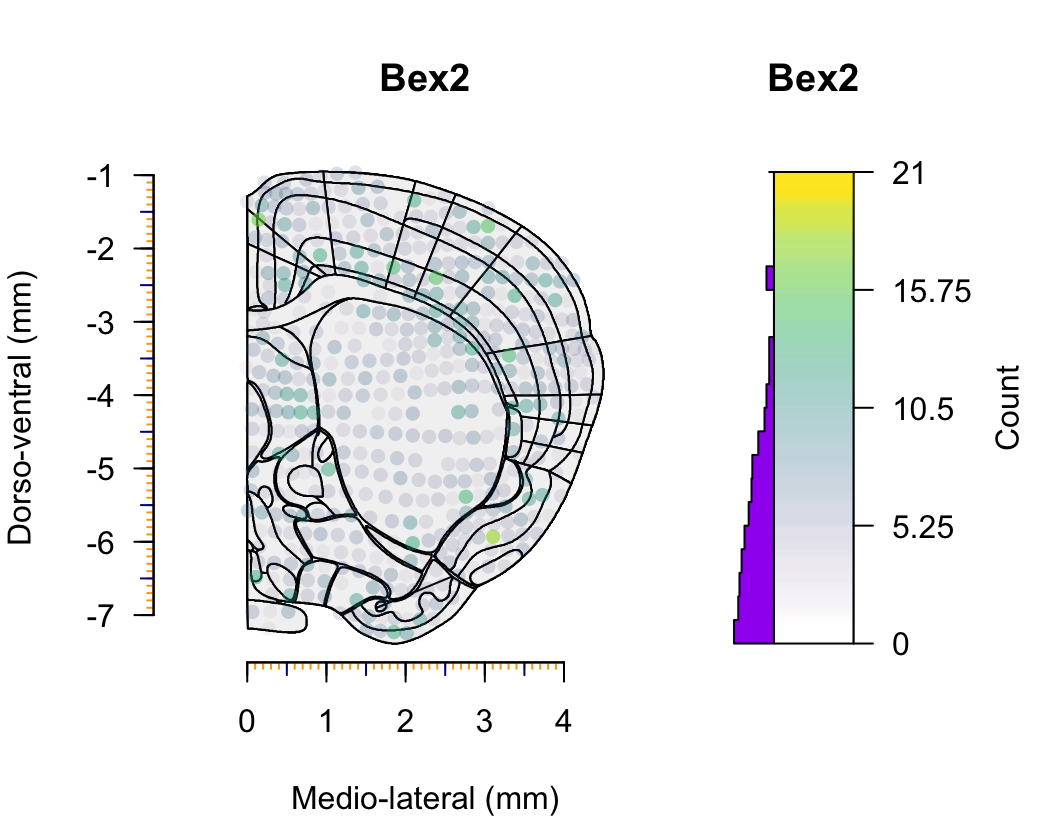
\includegraphics{wholebrain-bookdown_files/figure-latex/unnamed-chunk-13-6.pdf}

\begin{verbatim}
## Bex2
##  -----
##  Average number of Bex2 transcripts detected:
##  CPu : M = 3.17 ( SD = 2.02 ) molecules 
##  SS : M = 3.67 ( SD = 2.48 ) molecules
##  -----
## 
##  Welch Two Sample t-test
## 
## data:  CP and SS
## t = -1.7041, df = 232.63, p-value = 0.08969
## alternative hypothesis: true difference in means is not equal to 0
## 95 percent confidence interval:
##  -1.06886101  0.07740801
## sample estimates:
## mean of x mean of y 
##  3.170940  3.666667
\end{verbatim}

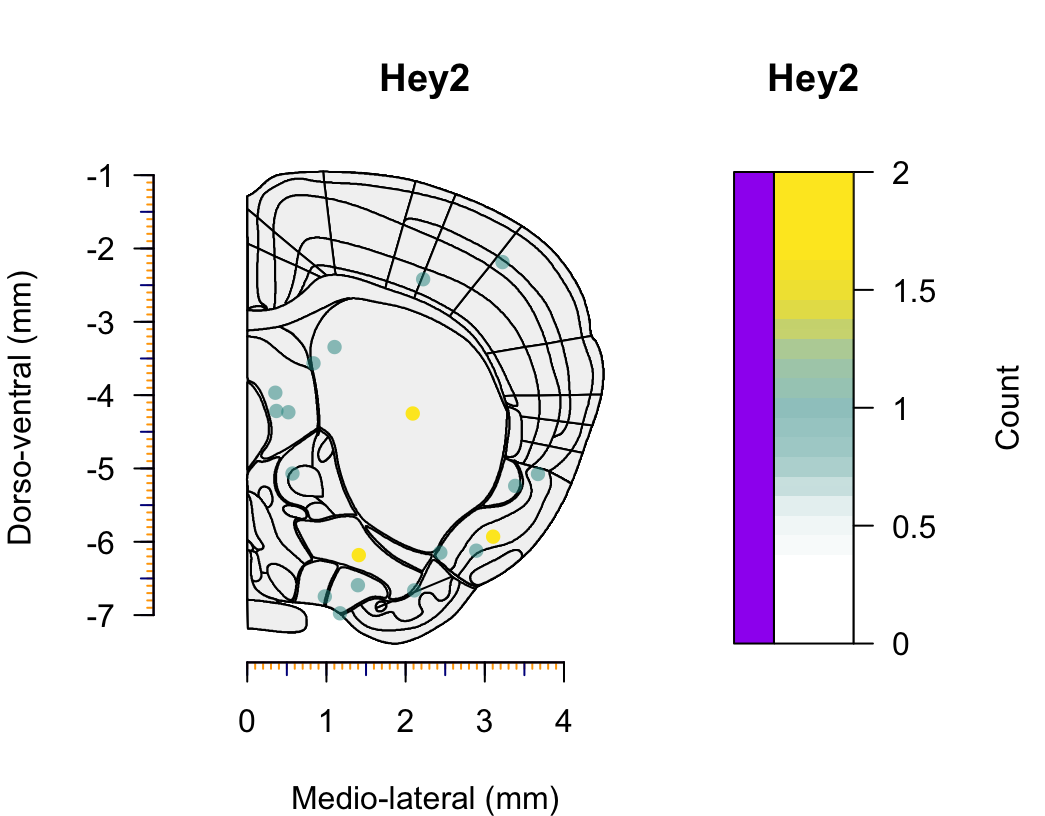
\includegraphics{wholebrain-bookdown_files/figure-latex/unnamed-chunk-13-7.pdf}

\begin{verbatim}
## Hey2
##  -----
##  Average number of Hey2 transcripts detected:
##  CPu : M = 0.03 ( SD = 0.22 ) molecules 
##  SS : M = 0.02 ( SD = 0.13 ) molecules
##  -----
## 
##  Welch Two Sample t-test
## 
## data:  CP and SS
## t = 0.75549, df = 181.22, p-value = 0.4509
## alternative hypothesis: true difference in means is not equal to 0
## 95 percent confidence interval:
##  -0.02889519  0.06475094
## sample estimates:
##  mean of x  mean of y 
## 0.03418803 0.01626016
\end{verbatim}

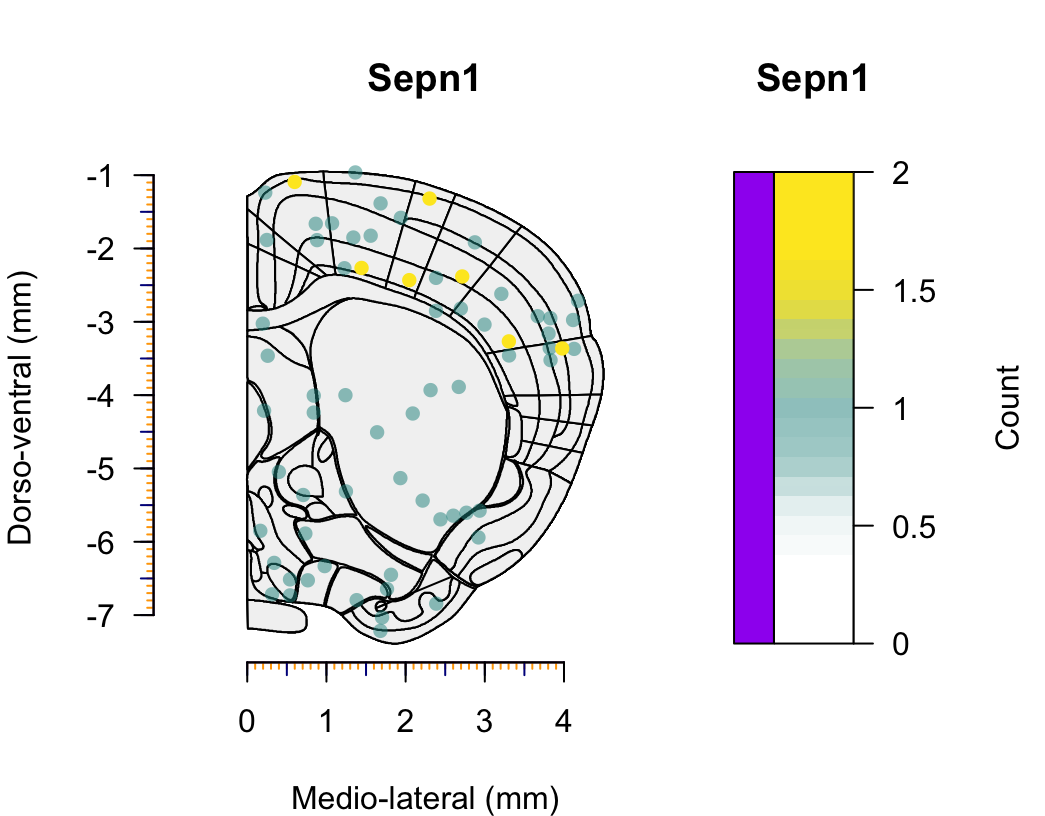
\includegraphics{wholebrain-bookdown_files/figure-latex/unnamed-chunk-13-8.pdf}

\begin{verbatim}
## Sepn1        █▬█ █ ▀█▀ MARKER FOR SOMATOSENSORY!
##  -----
##  Average number of Sepn1 transcripts detected:
##  CPu : M = 0.08 ( SD = 0.27 ) molecules 
##  SS : M = 0.2 ( SD = 0.49 ) molecules
##  -----
## 
##  Welch Two Sample t-test
## 
## data:  CP and SS
## t = -2.3335, df = 190.73, p-value = 0.02067
## alternative hypothesis: true difference in means is not equal to 0
## 95 percent confidence interval:
##  -0.21811251 -0.01828524
## sample estimates:
##  mean of x  mean of y 
## 0.07692308 0.19512195
\end{verbatim}

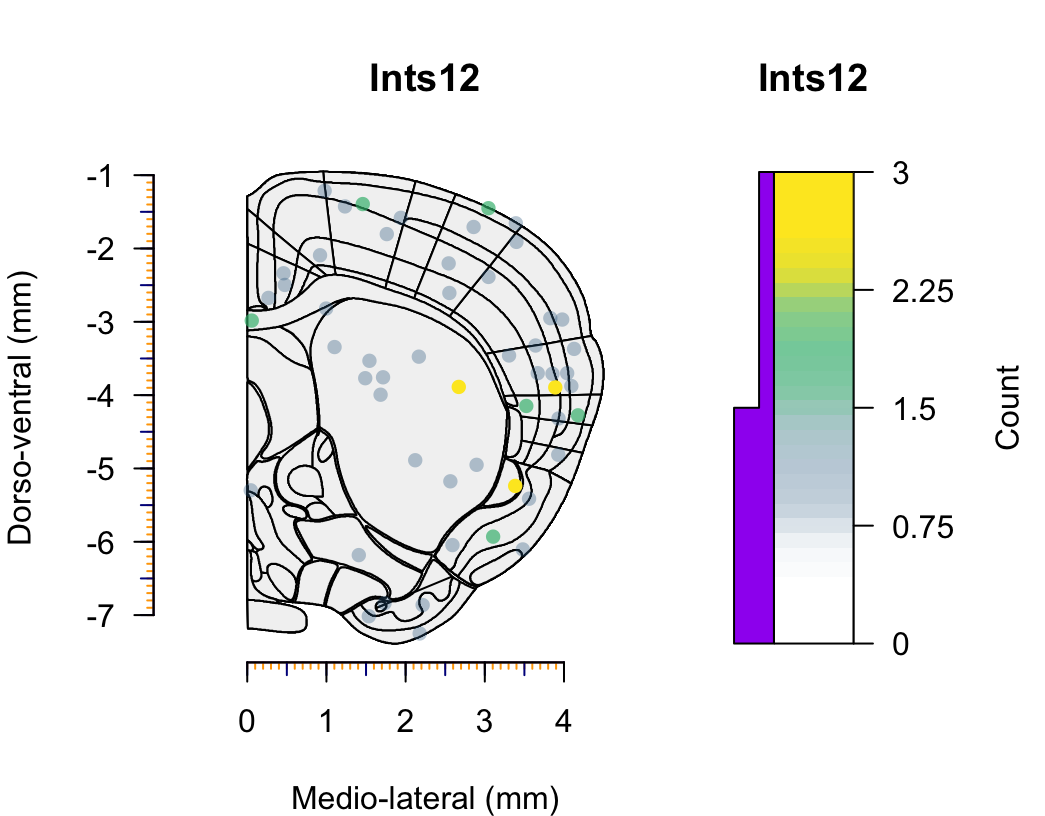
\includegraphics{wholebrain-bookdown_files/figure-latex/unnamed-chunk-13-9.pdf}

\begin{verbatim}
## Ints12
##  -----
##  Average number of Ints12 transcripts detected:
##  CPu : M = 0.1 ( SD = 0.38 ) molecules 
##  SS : M = 0.16 ( SD = 0.45 ) molecules
##  -----
## 
##  Welch Two Sample t-test
## 
## data:  CP and SS
## t = -1.1178, df = 234.72, p-value = 0.2648
## alternative hypothesis: true difference in means is not equal to 0
## 95 percent confidence interval:
##  -0.16585309  0.04577804
## sample estimates:
## mean of x mean of y 
## 0.1025641 0.1626016
\end{verbatim}

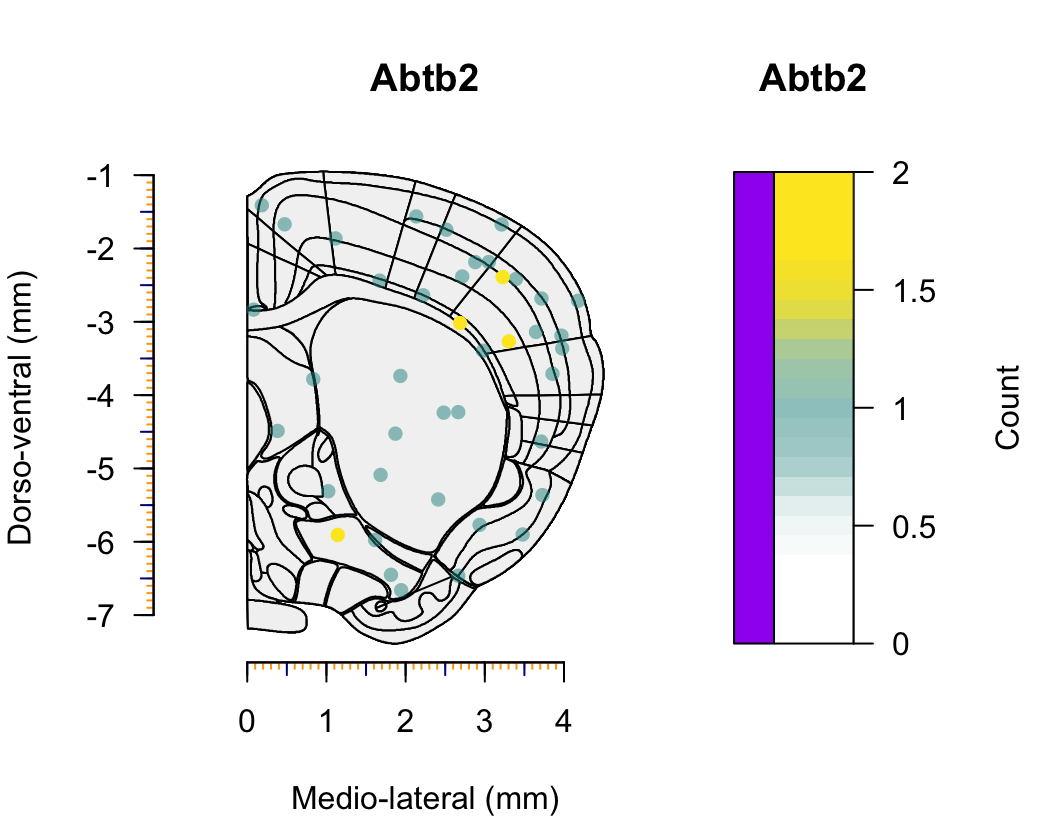
\includegraphics{wholebrain-bookdown_files/figure-latex/unnamed-chunk-13-10.pdf}

\begin{verbatim}
## Abtb2        █▬█ █ ▀█▀ MARKER FOR SOMATOSENSORY!
##  -----
##  Average number of Abtb2 transcripts detected:
##  CPu : M = 0.05 ( SD = 0.22 ) molecules 
##  SS : M = 0.16 ( SD = 0.43 ) molecules
##  -----
## 
##  Welch Two Sample t-test
## 
## data:  CP and SS
## t = -2.5304, df = 184.03, p-value = 0.01223
## alternative hypothesis: true difference in means is not equal to 0
## 95 percent confidence interval:
##  -0.19811407 -0.02452508
## sample estimates:
##  mean of x  mean of y 
## 0.05128205 0.16260163
\end{verbatim}

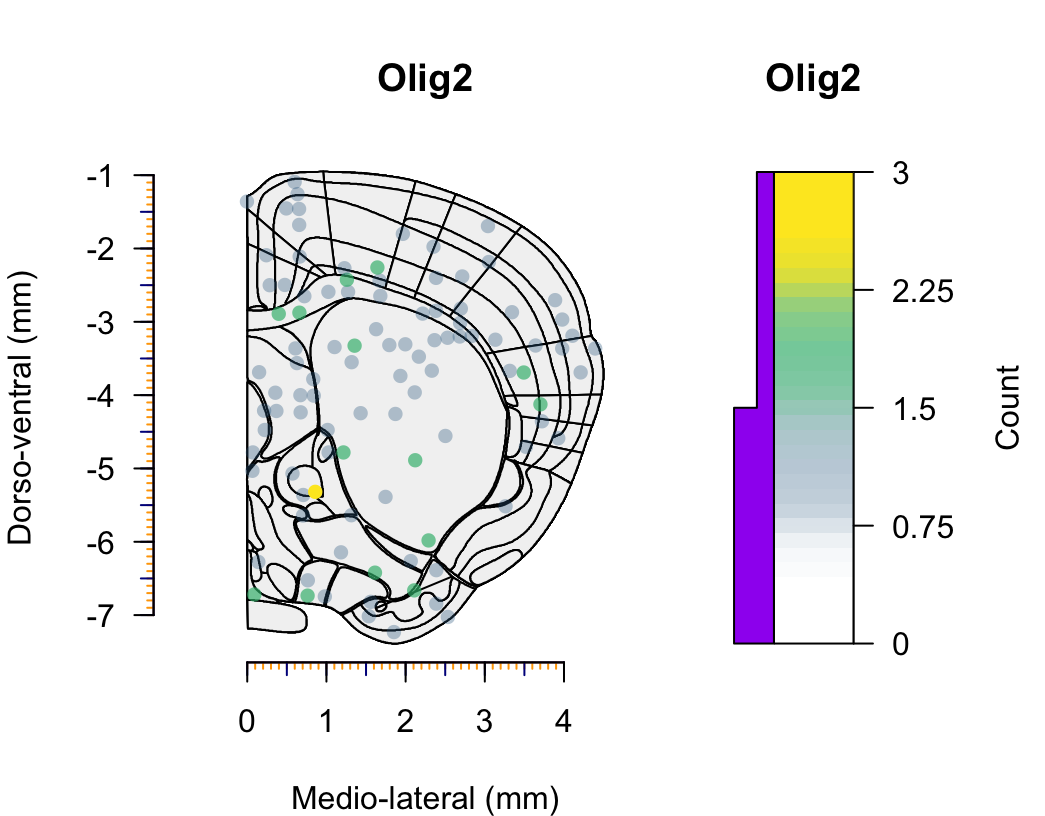
\includegraphics{wholebrain-bookdown_files/figure-latex/unnamed-chunk-13-11.pdf}

\begin{verbatim}
## Olig2
##  -----
##  Average number of Olig2 transcripts detected:
##  CPu : M = 0.21 ( SD = 0.49 ) molecules 
##  SS : M = 0.16 ( SD = 0.39 ) molecules
##  -----
## 
##  Welch Two Sample t-test
## 
## data:  CP and SS
## t = 0.8908, df = 222.36, p-value = 0.374
## alternative hypothesis: true difference in means is not equal to 0
## 95 percent confidence interval:
##  -0.06191493  0.16406211
## sample estimates:
## mean of x mean of y 
## 0.2136752 0.1626016
\end{verbatim}

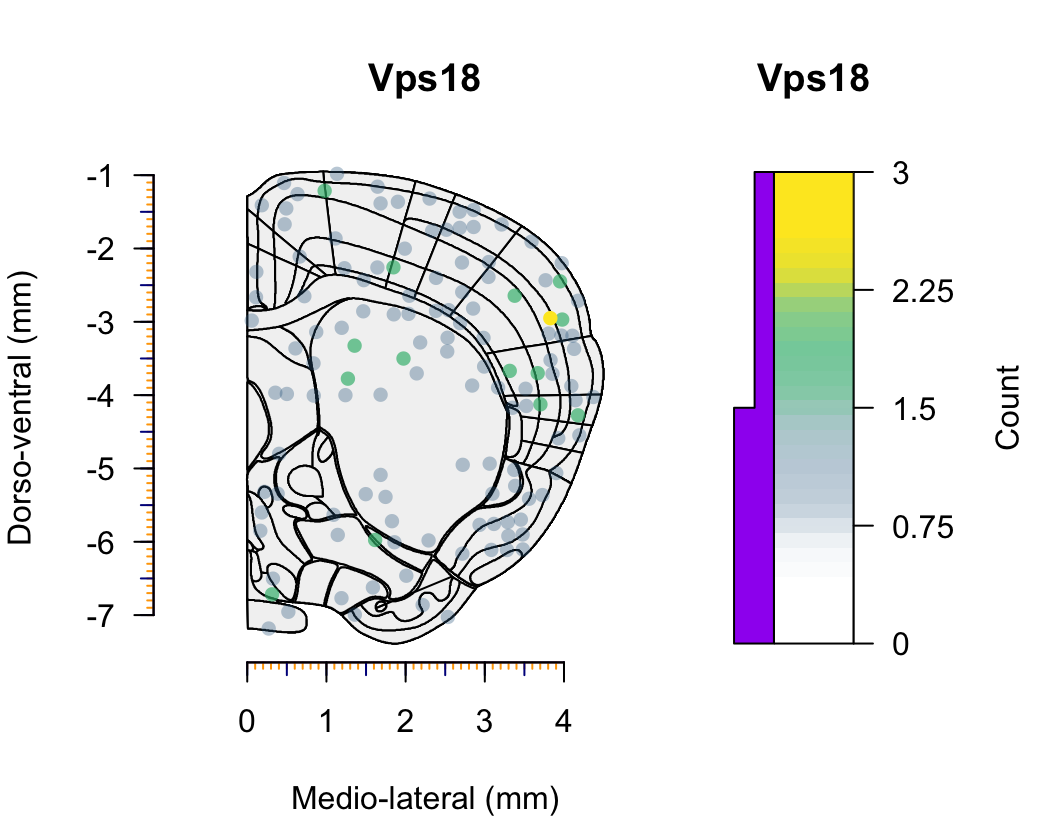
\includegraphics{wholebrain-bookdown_files/figure-latex/unnamed-chunk-13-12.pdf}

\begin{verbatim}
## Vps18        █▬█ █ ▀█▀ MARKER FOR SOMATOSENSORY!
##  -----
##  Average number of Vps18 transcripts detected:
##  CPu : M = 0.23 ( SD = 0.48 ) molecules 
##  SS : M = 0.37 ( SD = 0.62 ) molecules
##  -----
## 
##  Welch Two Sample t-test
## 
## data:  CP and SS
## t = -2.0072, df = 228.85, p-value = 0.04591
## alternative hypothesis: true difference in means is not equal to 0
## 95 percent confidence interval:
##  -0.283802806 -0.002626212
## sample estimates:
## mean of x mean of y 
## 0.2307692 0.3739837
\end{verbatim}

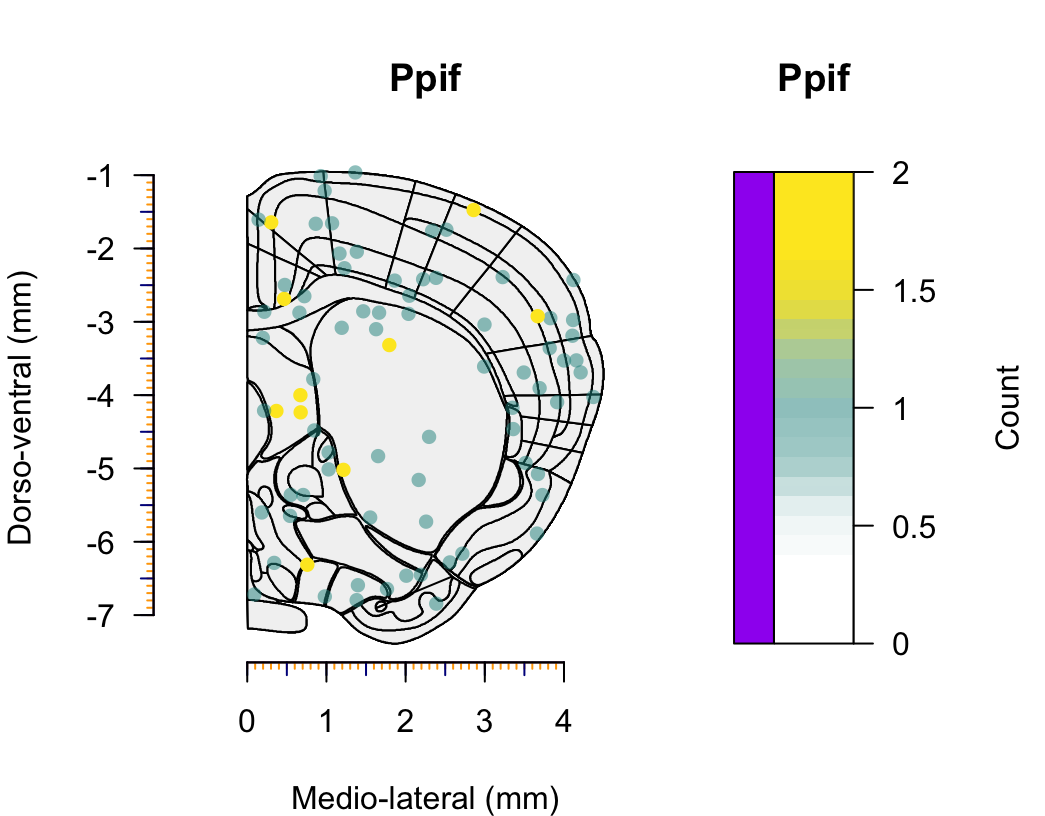
\includegraphics{wholebrain-bookdown_files/figure-latex/unnamed-chunk-13-13.pdf}

\begin{verbatim}
## Ppif
##  -----
##  Average number of Ppif transcripts detected:
##  CPu : M = 0.13 ( SD = 0.38 ) molecules 
##  SS : M = 0.18 ( SD = 0.43 ) molecules
##  -----
## 
##  Welch Two Sample t-test
## 
## data:  CP and SS
## t = -0.96975, df = 237.34, p-value = 0.3332
## alternative hypothesis: true difference in means is not equal to 0
## 95 percent confidence interval:
##  -0.15356323  0.05224991
## sample estimates:
## mean of x mean of y 
## 0.1282051 0.1788618
\end{verbatim}

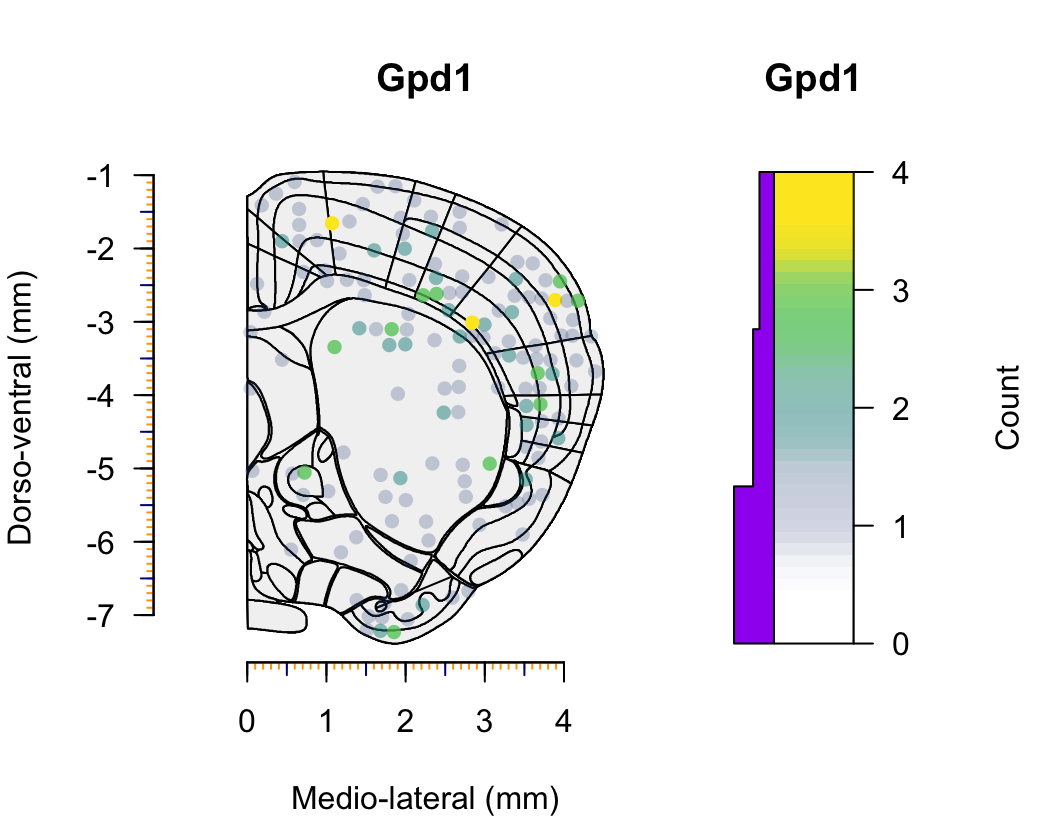
\includegraphics{wholebrain-bookdown_files/figure-latex/unnamed-chunk-13-14.pdf}

\begin{verbatim}
## Gpd1        █▬█ █ ▀█▀ MARKER FOR SOMATOSENSORY!
##  -----
##  Average number of Gpd1 transcripts detected:
##  CPu : M = 0.35 ( SD = 0.7 ) molecules 
##  SS : M = 0.63 ( SD = 0.91 ) molecules
##  -----
## 
##  Welch Two Sample t-test
## 
## data:  CP and SS
## t = -2.721, df = 228.2, p-value = 0.007011
## alternative hypothesis: true difference in means is not equal to 0
## 95 percent confidence interval:
##  -0.48917663 -0.07826135
## sample estimates:
## mean of x mean of y 
## 0.3504274 0.6341463
\end{verbatim}

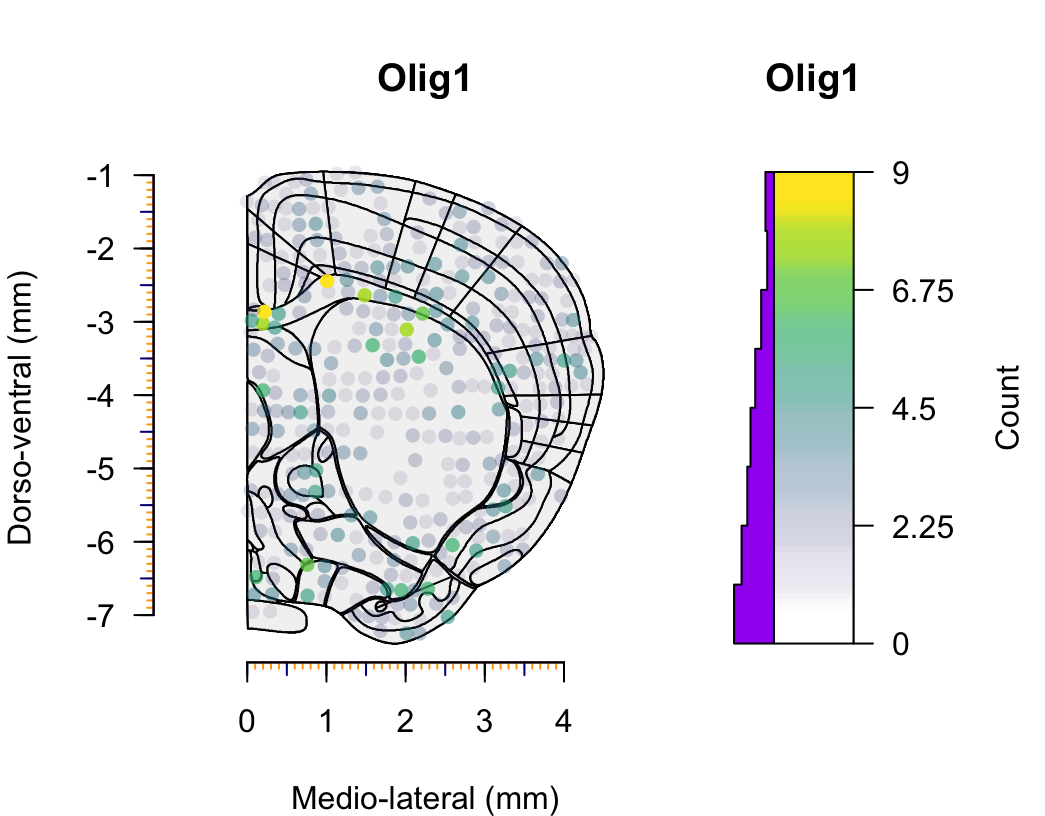
\includegraphics{wholebrain-bookdown_files/figure-latex/unnamed-chunk-13-15.pdf}

\begin{verbatim}
## Olig1
##  -----
##  Average number of Olig1 transcripts detected:
##  CPu : M = 1.38 ( SD = 1.49 ) molecules 
##  SS : M = 1.29 ( SD = 1.34 ) molecules
##  -----
## 
##  Welch Two Sample t-test
## 
## data:  CP and SS
## t = 0.45585, df = 232.13, p-value = 0.6489
## alternative hypothesis: true difference in means is not equal to 0
## 95 percent confidence interval:
##  -0.2770180  0.4437889
## sample estimates:
## mean of x mean of y 
##  1.376068  1.292683
\end{verbatim}

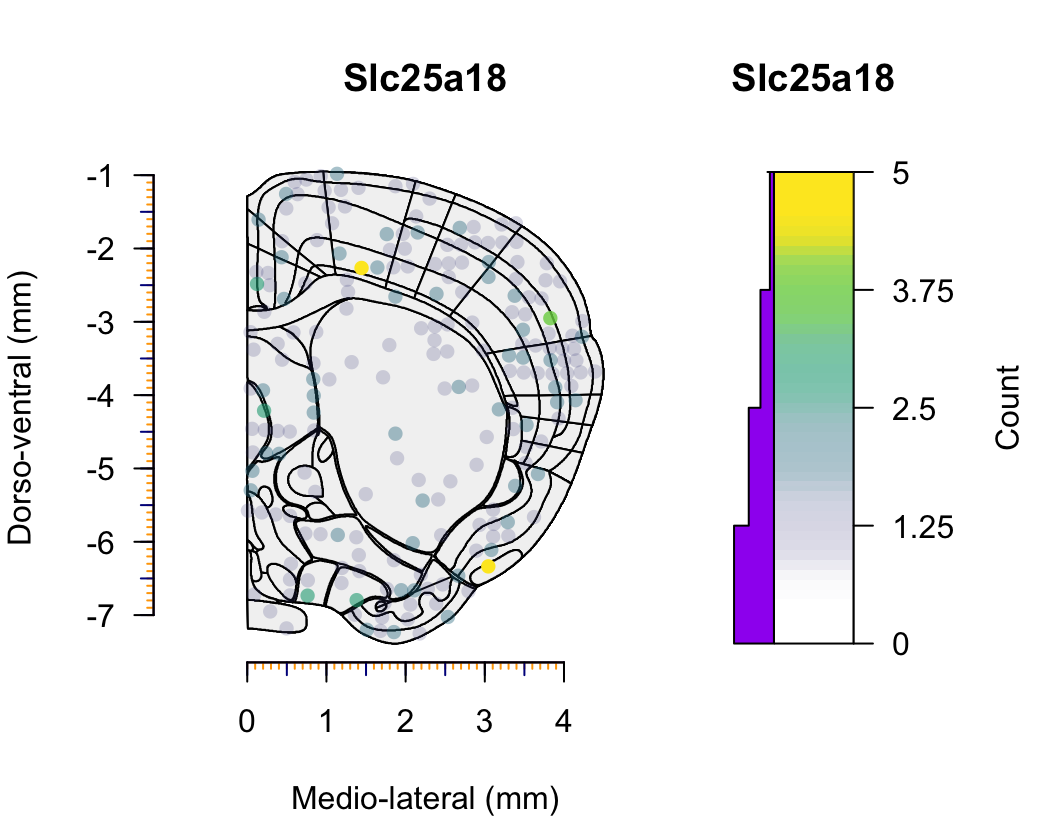
\includegraphics{wholebrain-bookdown_files/figure-latex/unnamed-chunk-13-16.pdf}

\begin{verbatim}
## Slc25a18        █▬█ █ ▀█▀ MARKER FOR SOMATOSENSORY!
##  -----
##  Average number of Slc25a18 transcripts detected:
##  CPu : M = 0.27 ( SD = 0.54 ) molecules 
##  SS : M = 0.62 ( SD = 0.73 ) molecules
##  -----
## 
##  Welch Two Sample t-test
## 
## data:  CP and SS
## t = -4.1812, df = 223.72, p-value = 4.164e-05
## alternative hypothesis: true difference in means is not equal to 0
## 95 percent confidence interval:
##  -0.5066931 -0.1820708
## sample estimates:
## mean of x mean of y 
## 0.2735043 0.6178862 
## 
## 
##  Nondetected genes: 
## 6330403K07Rik, Sntb1
\end{verbatim}

\subsection{Confirmatory conclusion:}\label{confirmatory-conclusion}

\begin{itemize}
\tightlist
\item
  Somatosensory:
\item
  \texttt{\{r\}\ cat(paste(conf.analysis\$somatosensory\ ,\ collapse=\textquotesingle{}\ ,\textquotesingle{}))}
\item
  Striatal:
\item
  \texttt{\{r\}\ cat(paste(conf.analysis\$striatum\ ,\ collapse=\textquotesingle{}\ ,\textquotesingle{}))}
\item
  Non detected:
\item
  \texttt{\{r\}\ cat(paste(conf.analysis\$non.detected\ ,\ collapse=\textquotesingle{}\ ,\textquotesingle{}))}
\end{itemize}

\subsection{Somatosensory:}\label{somatosensory}

\begin{Shaded}
\begin{Highlighting}[]
\KeywordTok{par}\NormalTok{(}\DataTypeTok{mfrow=}\KeywordTok{c}\NormalTok{(}\KeywordTok{length}\NormalTok{(conf.analysis$somatosensory)%/%}\DecValTok{4+1}\NormalTok{,}\DecValTok{4}\NormalTok\DecValTok{4+1}\NormalTok{), }\DataTypeTok{mar=}\KeywordTok{c}\NormalTok{(}\DecValTok{4}\NormalTok{,}\DecValTok{4}\NormalTok{,}\DecValTok{4}\NormalTok{,}\DecValTok{1}\NormalTok{))}
\KeywordTok{invisible}\NormalTok{(}\KeywordTok{sapply}\NormalTok{(conf.analysis$somatosensory, function(x)}\KeywordTok{plot.gene}\NormalTok{(dataset, regi, }\DataTypeTok{gene=}\NormalTok{x, }\DataTypeTok{colorfunc=}\NormalTok{viridis)))}
\end{Highlighting}
\end{Shaded}

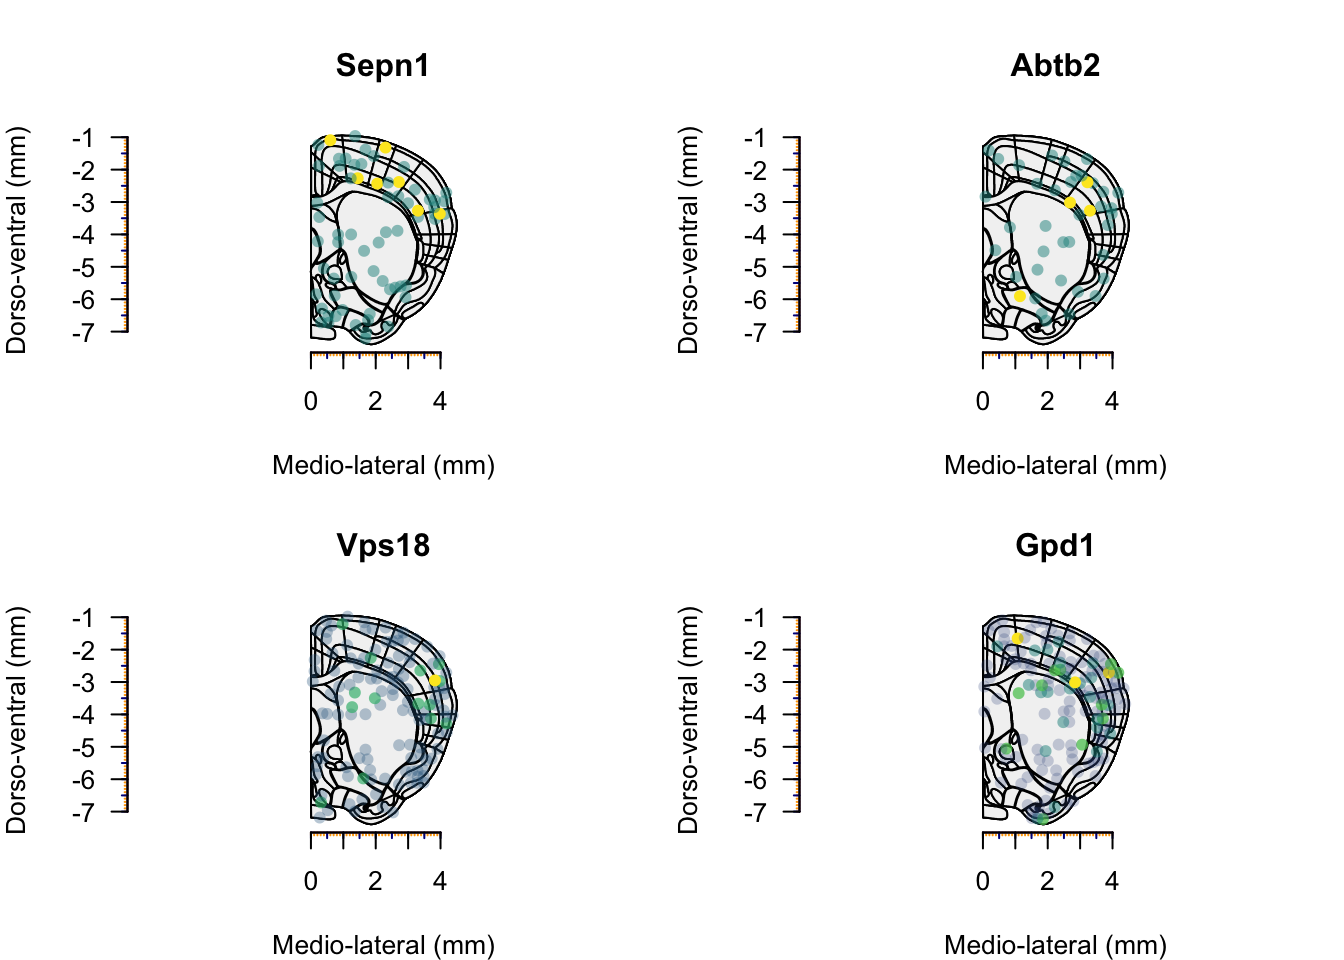
\includegraphics{wholebrain-bookdown_files/figure-latex/unnamed-chunk-14-1.pdf}
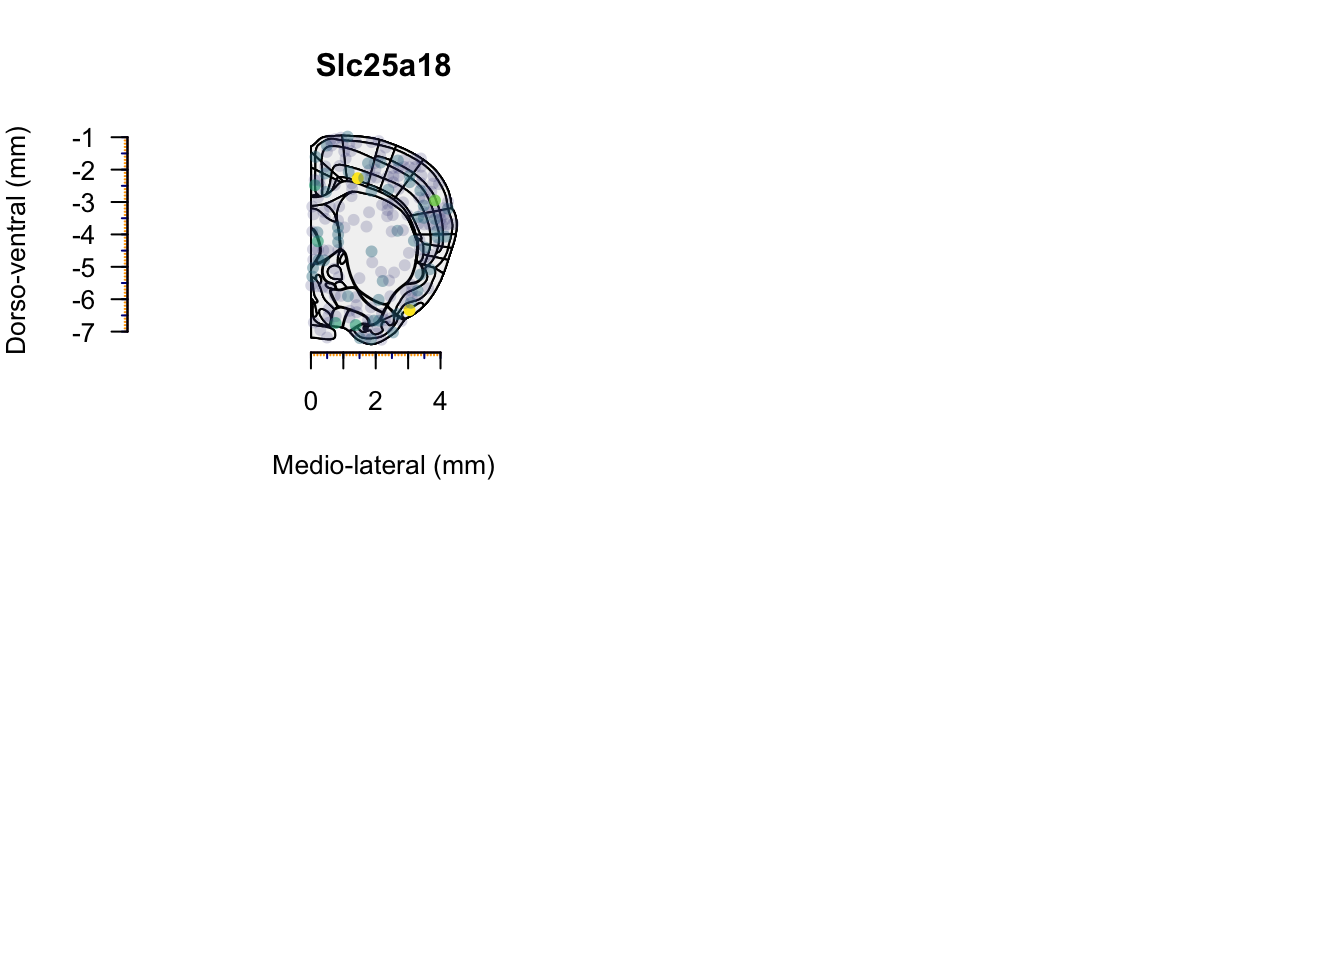
\includegraphics{wholebrain-bookdown_files/figure-latex/unnamed-chunk-14-2.pdf}

\subsection{Striatal:}\label{striatal}

\begin{Shaded}
\begin{Highlighting}[]
\KeywordTok{par}\NormalTok{(}\DataTypeTok{mfrow=}\KeywordTok{c}\NormalTok{(}\KeywordTok{length}\NormalTok{(conf.analysis$striatum)%/%}\DecValTok{4+1}\NormalTok{,}\DecValTok{4}\NormalTok{), }\DataTypeTok{mar=}\KeywordTok{c}\NormalTok{(}\DecValTok{4}\NormalTok{,}\DecValTok{4}\NormalTok{,}\DecValTok{4}\NormalTok{,}\DecValTok{1}\NormalTok{))}
\KeywordTok{invisible}\NormalTok{(}\KeywordTok{sapply}\NormalTok{(conf.analysis$striatum, function(x)}\KeywordTok{plot.gene}\NormalTok{(dataset, regi, }\DataTypeTok{gene=}\NormalTok{x, }\DataTypeTok{colorfunc=}\NormalTok{viridis)))}
\end{Highlighting}
\end{Shaded}

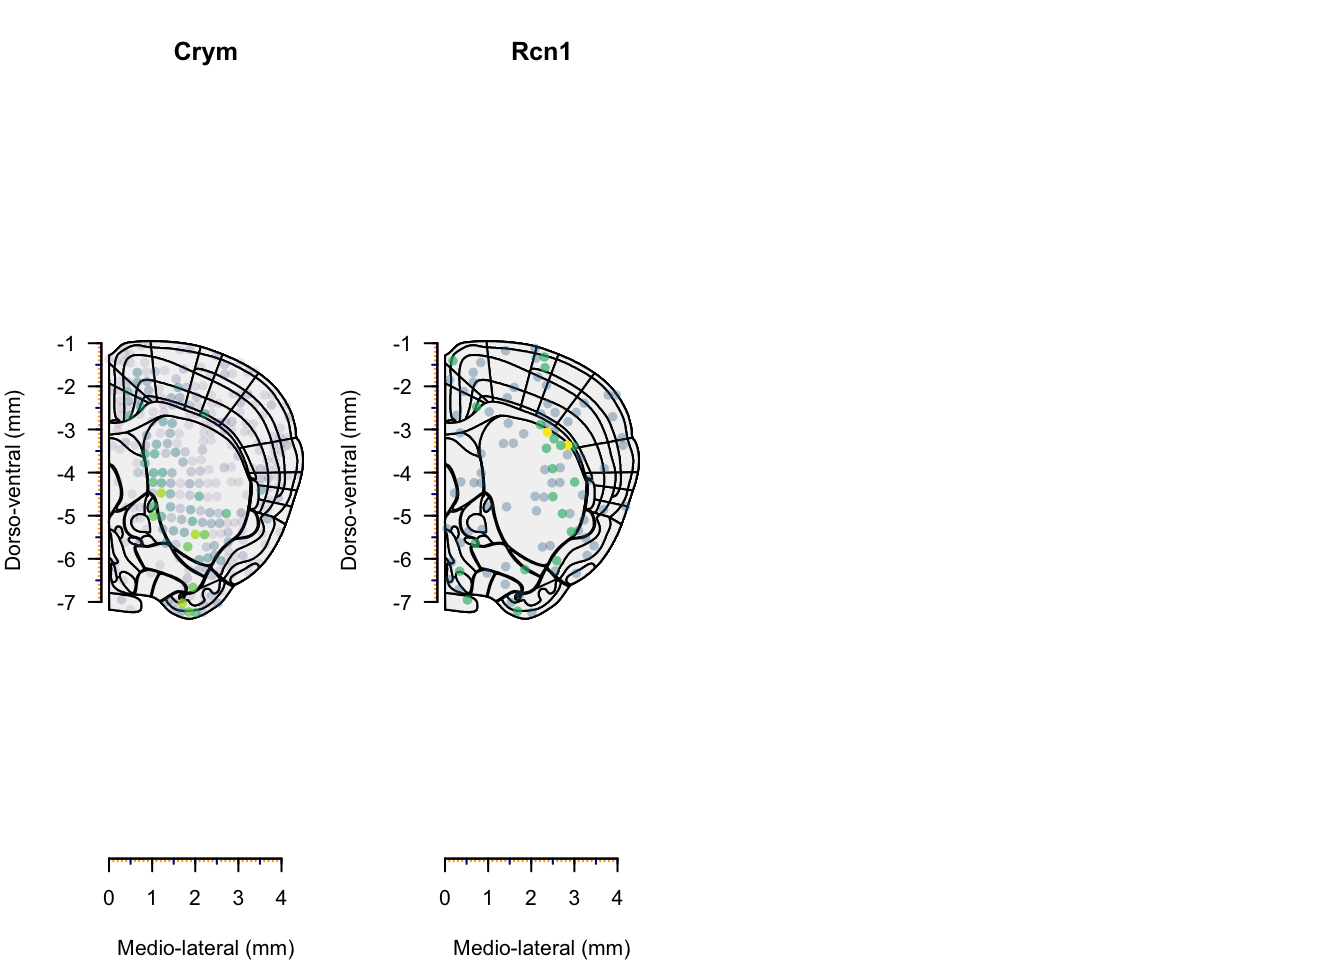
\includegraphics{wholebrain-bookdown_files/figure-latex/unnamed-chunk-15-1.pdf}

\section{Exploratory analysis}\label{exploratory-analysis}

Now lets run for some other genes:

\begin{Shaded}
\begin{Highlighting}[]
\CommentTok{#Genes that are differentially expressed between striatal and somatosensory cortical astrocytes:}
\NormalTok{genes.of.interest<-}\KeywordTok{c}\NormalTok{(}\StringTok{"Adm"}\NormalTok{, }\StringTok{"Gdf11"}\NormalTok{, }\StringTok{"Mstn"}\NormalTok{, }\StringTok{"Bmp3"}\NormalTok{, }\StringTok{"Gdf10"}\NormalTok{, }\StringTok{"Gdf2"}\NormalTok{, }\StringTok{"Bmp10"}\NormalTok{, }\StringTok{"Gdf6"}\NormalTok{, }\StringTok{"Gdf5"}\NormalTok{, }\StringTok{"Gdf7"}\NormalTok{, }\StringTok{"Bmp5"}\NormalTok{, }\StringTok{"Bmp6"}\NormalTok{, }\StringTok{"Bmp7"}\NormalTok{, }\StringTok{"Bmp8a"}\NormalTok{, }\StringTok{"Bmp8b"}\NormalTok{, }\StringTok{"Bmp2"}\NormalTok{, }\StringTok{"Bmp4"}\NormalTok{, }\StringTok{"Cntf"}\NormalTok{, }\StringTok{"Lif"}\NormalTok{, }\StringTok{"Il6"}\NormalTok{, }\StringTok{"Csf1"}\NormalTok{, }\StringTok{"Csf3"}\NormalTok{, }\StringTok{"Csf2"}\NormalTok{, }\StringTok{"Egf"}\NormalTok{, }\StringTok{"Efna1"}\NormalTok{, }\StringTok{"Efna2"}\NormalTok{, }\StringTok{"Efna3"}\NormalTok{, }\StringTok{"Efna4"}\NormalTok{, }\StringTok{"Efna5"}\NormalTok{, }\StringTok{"Efnb1"}\NormalTok{, }\StringTok{"Efnb2"}\NormalTok{, }\StringTok{"Efnb3"}\NormalTok{, }\StringTok{"Epo"}\NormalTok{, }\StringTok{"Fgf1"}\NormalTok{, }\StringTok{"Fgf2"}\NormalTok{, }\StringTok{"Fgf3"}\NormalTok{, }\StringTok{"Fgf4"}\NormalTok{, }\StringTok{"Fgf5"}\NormalTok{, }\StringTok{"Fgf6"}\NormalTok{, }\StringTok{"Fgf7"}\NormalTok{, }\StringTok{"Fgf8"}\NormalTok{, }\StringTok{"Fgf9"}\NormalTok{, }\StringTok{"Fgf10"}\NormalTok{, }\StringTok{"Fgf11"}\NormalTok{, }\StringTok{"Fgf12"}\NormalTok{, }\StringTok{"Fgf13"}\NormalTok{, }\StringTok{"Fgf14"}\NormalTok{, }\StringTok{"Fgf16"}\NormalTok{, }\StringTok{"Fgf17"}\NormalTok{, }\StringTok{"Fgf18"}\NormalTok{, }\StringTok{"Fgf19"}\NormalTok{, }\StringTok{"Fgf20"}\NormalTok{, }\StringTok{"Fgf21"}\NormalTok{, }\StringTok{"Fgf22"}\NormalTok{, }\StringTok{"Fgf23"}\NormalTok{, }\StringTok{"Gdnf"}\NormalTok{, }\StringTok{"Nrtn"}\NormalTok{, }\StringTok{"Pspn"}\NormalTok{, }\StringTok{"Artn"}\NormalTok{, }\StringTok{"Gdf9"}\NormalTok{, }\StringTok{"Hgf"}\NormalTok{, }\StringTok{"Hdgf"}\NormalTok{, }\StringTok{"Ins"}\NormalTok{, }\StringTok{"Igf1"}\NormalTok{, }\StringTok{"Igf2"}\NormalTok{, }\StringTok{"Il1a"}\NormalTok{, }\StringTok{"Il1b"}\NormalTok{, }\StringTok{"Il2"}\NormalTok{, }\StringTok{"Il3"}\NormalTok{, }\StringTok{"Il4"}\NormalTok{, }\StringTok{"Il5"}\NormalTok{, }\StringTok{"Il6"}\NormalTok{, }\StringTok{"Il7"}\NormalTok{, }\StringTok{"Nrg1"}\NormalTok{, }\StringTok{"Nrg2"}\NormalTok{, }\StringTok{"Nrg3"}\NormalTok{, }\StringTok{"Nrg4"}\NormalTok{, }\StringTok{"Bdnf"}\NormalTok{, }\StringTok{"Ngf"}\NormalTok{, }\StringTok{"Ntf3"}\NormalTok{, }\StringTok{"Ntf4"}\NormalTok{, }\StringTok{"Pgf"}\NormalTok{, }\StringTok{"Pdgfa"}\NormalTok{, }\StringTok{"Pdgfb"}\NormalTok{, }\StringTok{"Rnls"}\NormalTok{, }\StringTok{"Tpo"}\NormalTok{, }\StringTok{"Tgfa"}\NormalTok{, }\StringTok{"Tgfb1"}\NormalTok{, }\StringTok{"Tgfb2"}\NormalTok{, }\StringTok{"Tgfb3"}\NormalTok{, }\StringTok{"Tnf"}\NormalTok{, }\StringTok{"Vegfa"}\NormalTok{, }\StringTok{"Vegfb"}\NormalTok{, }\StringTok{"Vegfc"}\NormalTok{, }\StringTok{"Vegfd"}\NormalTok{, }\StringTok{"Wnt1"}\NormalTok{, }\StringTok{"Wnt2"}\NormalTok{, }\StringTok{"Wnt2b"}\NormalTok{, }\StringTok{"Wnt13"}\NormalTok{, }\StringTok{"Wnt3a"}\NormalTok{, }\StringTok{"Wnt4"}\NormalTok{, }\StringTok{"Wnt5a"}\NormalTok{, }\StringTok{"Wnt5b"}\NormalTok{, }\StringTok{"Wnt6"}\NormalTok{, }\StringTok{"Wnt7a"}\NormalTok{, }\StringTok{"Wnt7b"}\NormalTok{, }\StringTok{"Wnt8a"}\NormalTok{, }\StringTok{"Wnt8b"}\NormalTok{, }\StringTok{"Wnt9a"}\NormalTok{, }\StringTok{"Wnt9b"}\NormalTok{, }\StringTok{"Wnt10a"}\NormalTok{, }\StringTok{"Wnt10b"}\NormalTok{, }\StringTok{"Wnt11"}\NormalTok{, }\StringTok{"Wnt16"}\NormalTok{, }\StringTok{"Penk"}\NormalTok{)}

\NormalTok{expl.analysis<-}\KeywordTok{plot.these.genes}\NormalTok{(genes.of.interest)}
\end{Highlighting}
\end{Shaded}

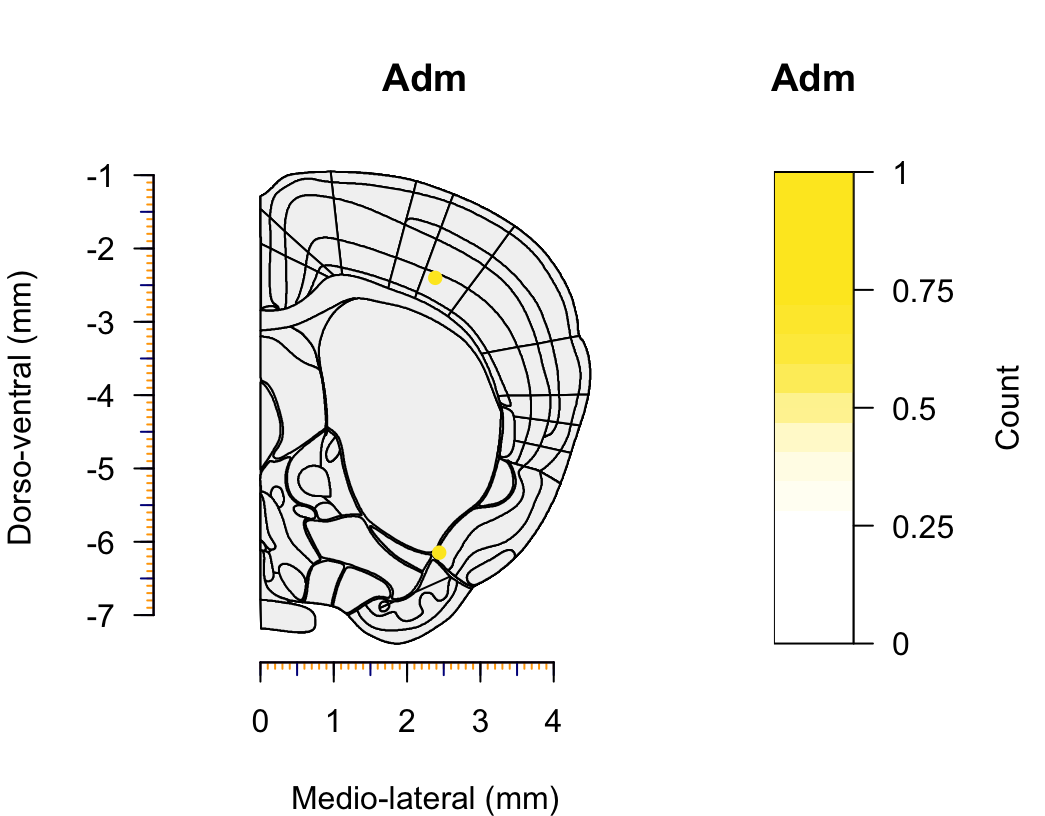
\includegraphics{wholebrain-bookdown_files/figure-latex/unnamed-chunk-16-1.pdf}

\begin{verbatim}
## Adm
##  -----
##  Average number of Adm transcripts detected:
##  CPu : M = 0 ( SD = 0 ) molecules 
##  SS : M = 0.01 ( SD = 0.09 ) molecules
##  -----
## 
##  Welch Two Sample t-test
## 
## data:  CP and SS
## t = -1, df = 122, p-value = 0.3193
## alternative hypothesis: true difference in means is not equal to 0
## 95 percent confidence interval:
##  -0.024224389  0.007964227
## sample estimates:
##   mean of x   mean of y 
## 0.000000000 0.008130081
\end{verbatim}

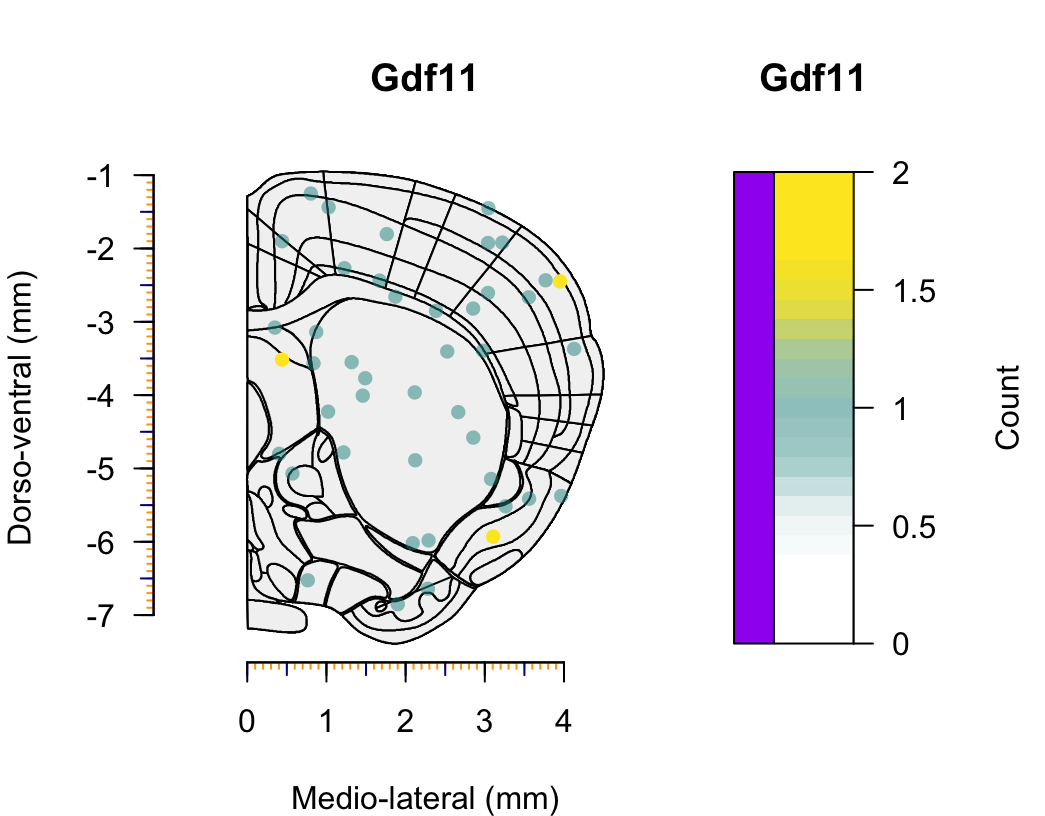
\includegraphics{wholebrain-bookdown_files/figure-latex/unnamed-chunk-16-2.pdf}

\begin{verbatim}
## Gdf11
##  -----
##  Average number of Gdf11 transcripts detected:
##  CPu : M = 0.13 ( SD = 0.34 ) molecules 
##  SS : M = 0.08 ( SD = 0.3 ) molecules
##  -----
## 
##  Welch Two Sample t-test
## 
## data:  CP and SS
## t = 1.1346, df = 232.57, p-value = 0.2577
## alternative hypothesis: true difference in means is not equal to 0
## 95 percent confidence interval:
##  -0.03454511  0.12835374
## sample estimates:
##  mean of x  mean of y 
## 0.12820513 0.08130081
\end{verbatim}

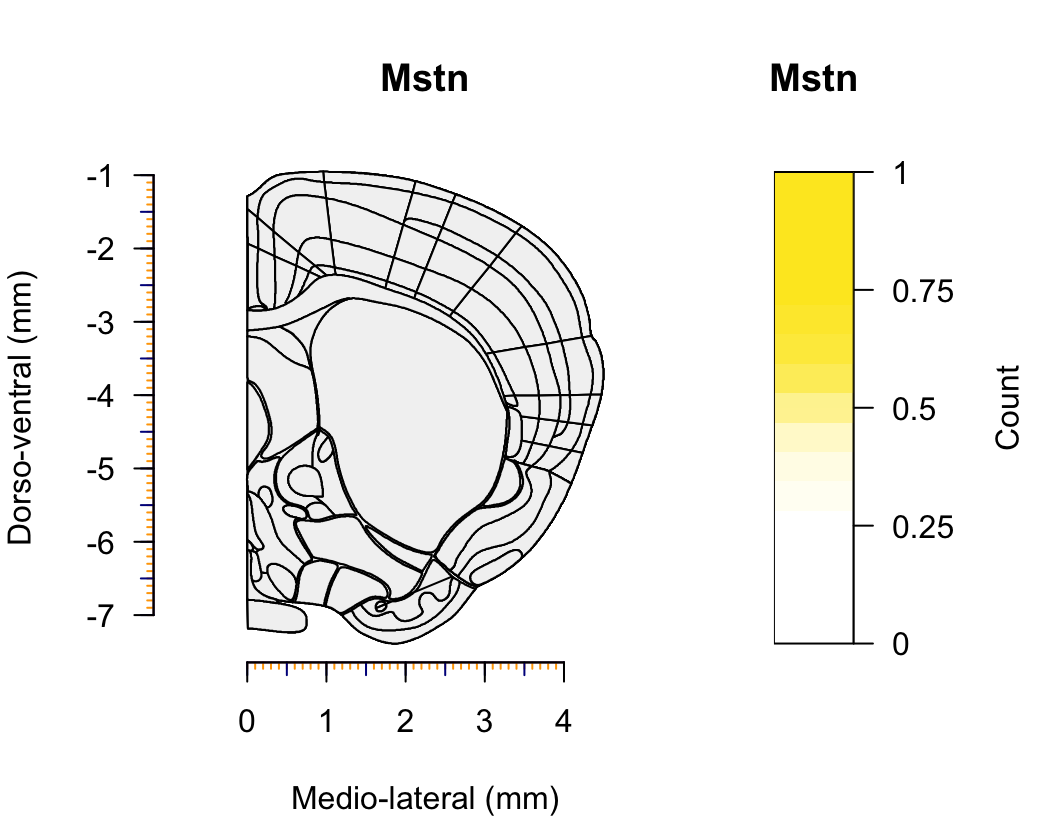
\includegraphics{wholebrain-bookdown_files/figure-latex/unnamed-chunk-16-3.pdf}

\begin{verbatim}
## Mstn
##  -----
##  Average number of Mstn transcripts detected:
##  CPu : M = 0 ( SD = 0 ) molecules 
##  SS : M = 0 ( SD = 0 ) molecules
##  -----
## 
##  Welch Two Sample t-test
## 
## data:  CP and SS
## t = NaN, df = NaN, p-value = NA
## alternative hypothesis: true difference in means is not equal to 0
## 95 percent confidence interval:
##  NaN NaN
## sample estimates:
## mean of x mean of y 
##         0         0
\end{verbatim}

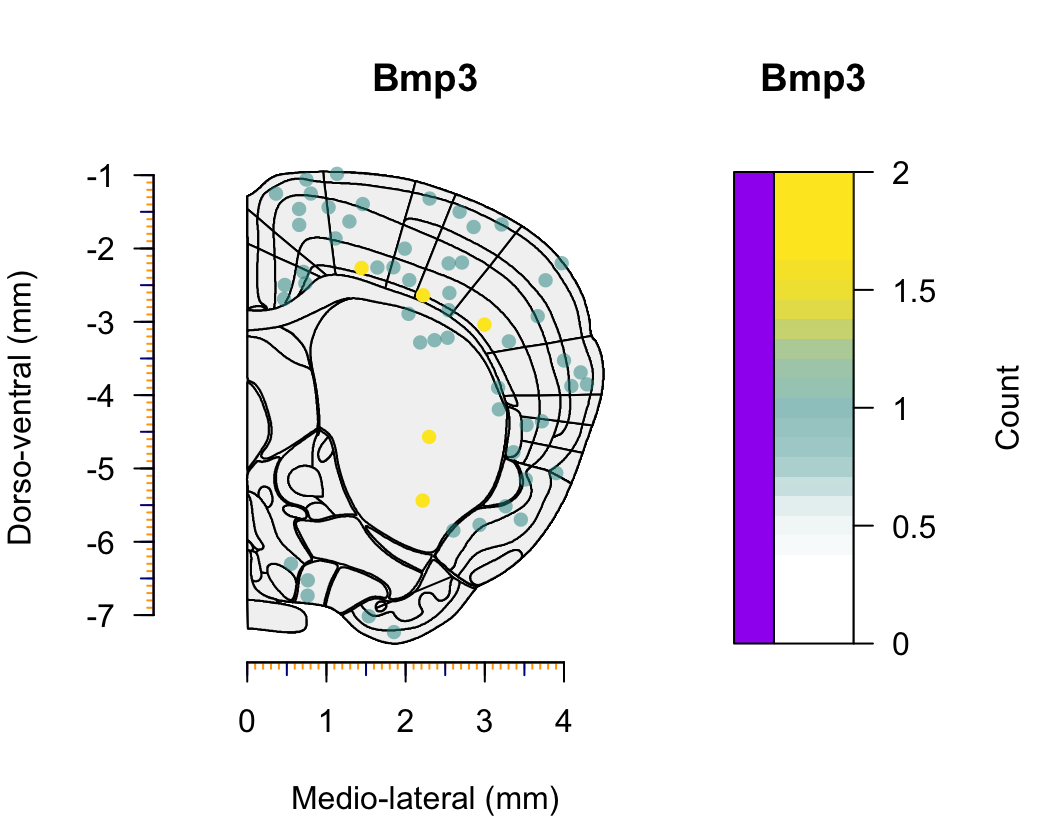
\includegraphics{wholebrain-bookdown_files/figure-latex/unnamed-chunk-16-4.pdf}

\begin{verbatim}
## Bmp3        █▬█ █ ▀█▀ MARKER FOR SOMATOSENSORY!
##  -----
##  Average number of Bmp3 transcripts detected:
##  CPu : M = 0.08 ( SD = 0.33 ) molecules 
##  SS : M = 0.19 ( SD = 0.43 ) molecules
##  -----
## 
##  Welch Two Sample t-test
## 
## data:  CP and SS
## t = -2.2377, df = 226.51, p-value = 0.02621
## alternative hypothesis: true difference in means is not equal to 0
## 95 percent confidence interval:
##  -0.20699456 -0.01314302
## sample estimates:
##  mean of x  mean of y 
## 0.07692308 0.18699187
\end{verbatim}

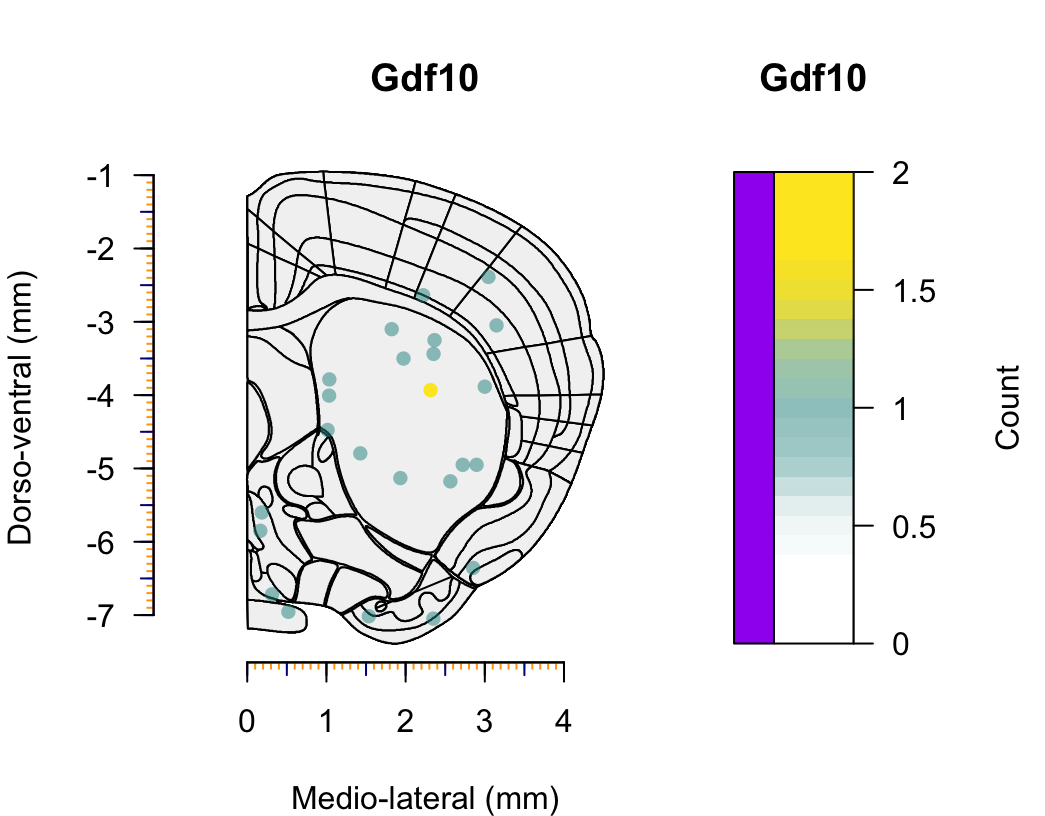
\includegraphics{wholebrain-bookdown_files/figure-latex/unnamed-chunk-16-5.pdf}

\begin{verbatim}
## Gdf10        █▬█ █ ▀█▀ MARKER FOR CAUDATE PUTAMEN!
##  -----
##  Average number of Gdf10 transcripts detected:
##  CPu : M = 0.13 ( SD = 0.36 ) molecules 
##  SS : M = 0.02 ( SD = 0.15 ) molecules
##  -----
## 
##  Welch Two Sample t-test
## 
## data:  CP and SS
## t = 2.8728, df = 155.74, p-value = 0.004637
## alternative hypothesis: true difference in means is not equal to 0
## 95 percent confidence interval:
##  0.03243176 0.17519801
## sample estimates:
##  mean of x  mean of y 
## 0.12820513 0.02439024
\end{verbatim}

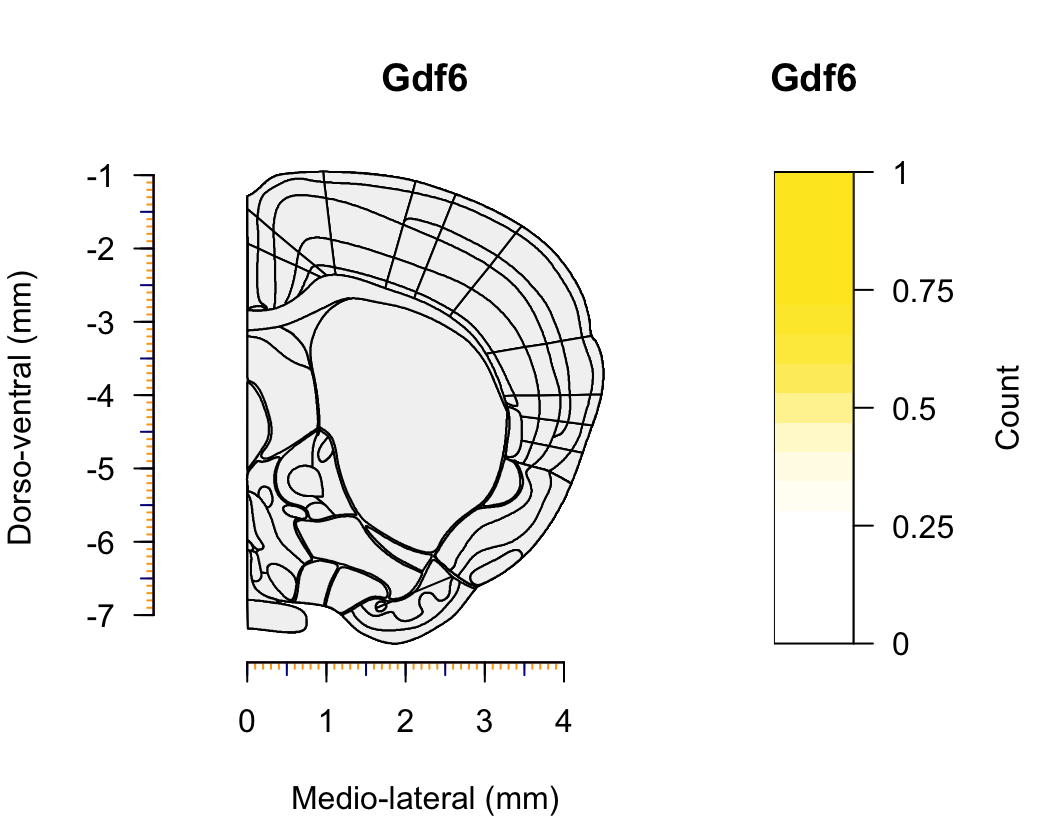
\includegraphics{wholebrain-bookdown_files/figure-latex/unnamed-chunk-16-6.pdf}

\begin{verbatim}
## Gdf6
##  -----
##  Average number of Gdf6 transcripts detected:
##  CPu : M = 0 ( SD = 0 ) molecules 
##  SS : M = 0 ( SD = 0 ) molecules
##  -----
## 
##  Welch Two Sample t-test
## 
## data:  CP and SS
## t = NaN, df = NaN, p-value = NA
## alternative hypothesis: true difference in means is not equal to 0
## 95 percent confidence interval:
##  NaN NaN
## sample estimates:
## mean of x mean of y 
##         0         0
\end{verbatim}

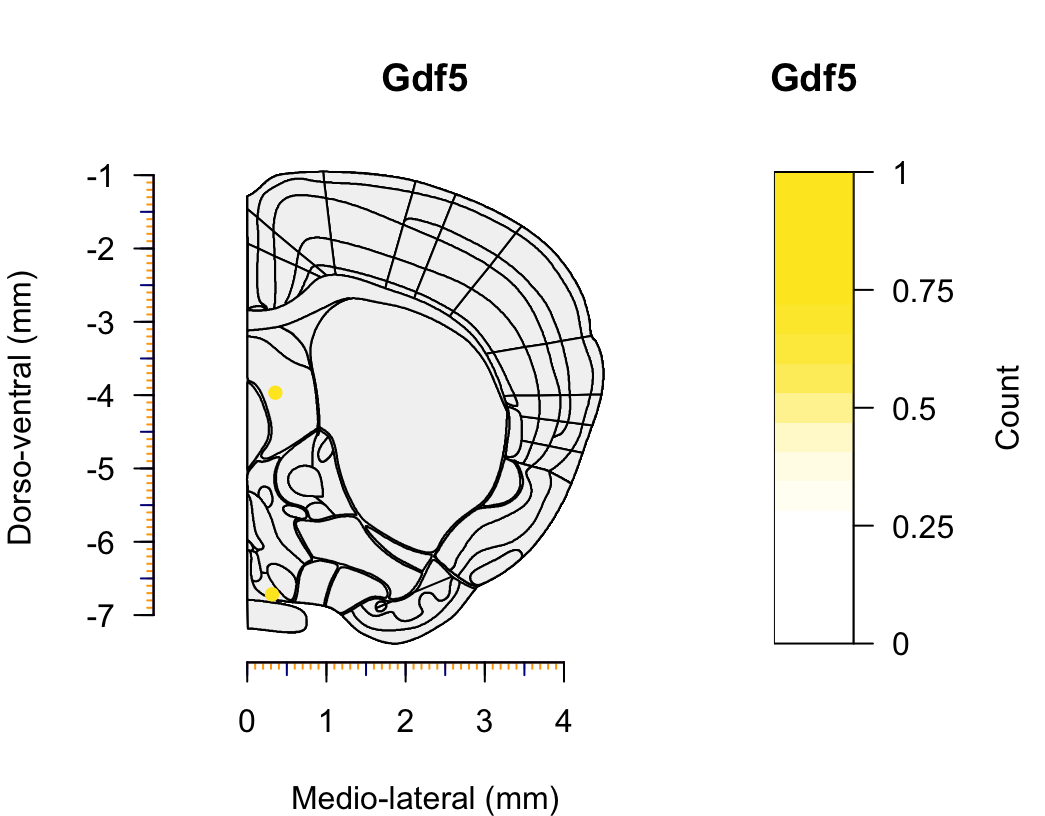
\includegraphics{wholebrain-bookdown_files/figure-latex/unnamed-chunk-16-7.pdf}

\begin{verbatim}
## Gdf5
##  -----
##  Average number of Gdf5 transcripts detected:
##  CPu : M = 0 ( SD = 0 ) molecules 
##  SS : M = 0 ( SD = 0 ) molecules
##  -----
## 
##  Welch Two Sample t-test
## 
## data:  CP and SS
## t = NaN, df = NaN, p-value = NA
## alternative hypothesis: true difference in means is not equal to 0
## 95 percent confidence interval:
##  NaN NaN
## sample estimates:
## mean of x mean of y 
##         0         0
\end{verbatim}

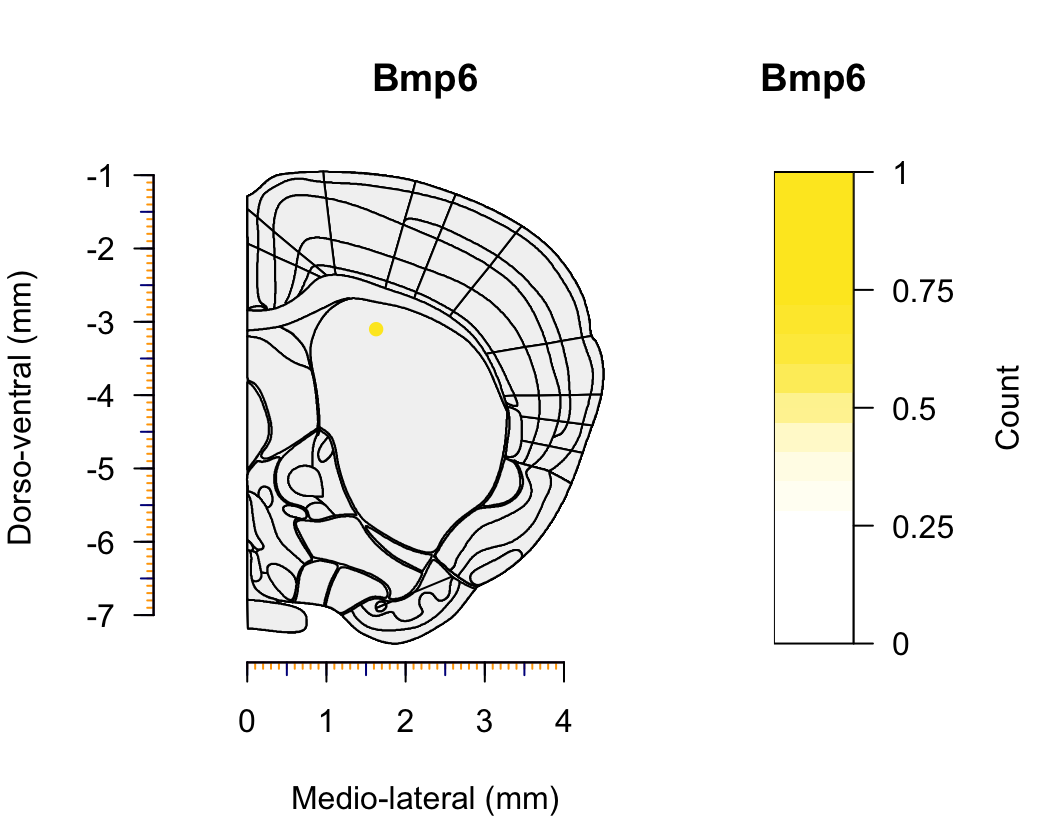
\includegraphics{wholebrain-bookdown_files/figure-latex/unnamed-chunk-16-8.pdf}

\begin{verbatim}
## Bmp6
##  -----
##  Average number of Bmp6 transcripts detected:
##  CPu : M = 0.01 ( SD = 0.09 ) molecules 
##  SS : M = 0 ( SD = 0 ) molecules
##  -----
## 
##  Welch Two Sample t-test
## 
## data:  CP and SS
## t = 1, df = 116, p-value = 0.3194
## alternative hypothesis: true difference in means is not equal to 0
## 95 percent confidence interval:
##  -0.008381419  0.025475436
## sample estimates:
##   mean of x   mean of y 
## 0.008547009 0.000000000
\end{verbatim}

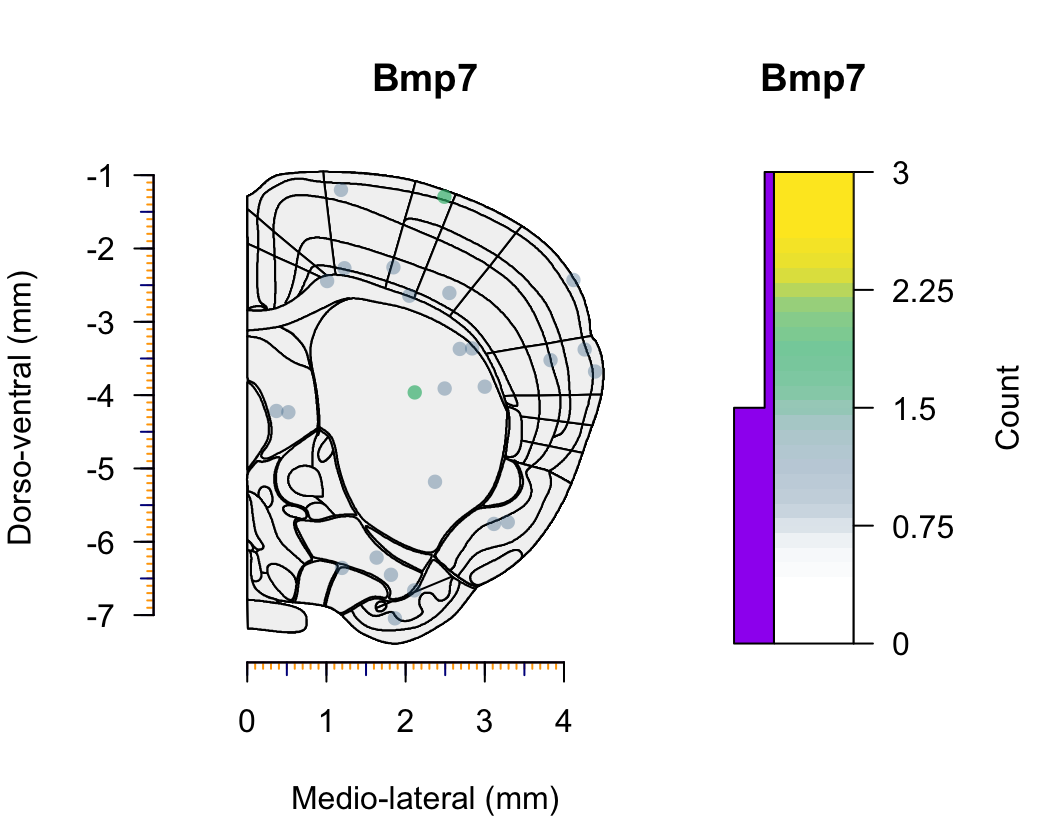
\includegraphics{wholebrain-bookdown_files/figure-latex/unnamed-chunk-16-9.pdf}

\begin{verbatim}
## Bmp7
##  -----
##  Average number of Bmp7 transcripts detected:
##  CPu : M = 0.06 ( SD = 0.27 ) molecules 
##  SS : M = 0.07 ( SD = 0.29 ) molecules
##  -----
## 
##  Welch Two Sample t-test
## 
## data:  CP and SS
## t = -0.36702, df = 237.92, p-value = 0.7139
## alternative hypothesis: true difference in means is not equal to 0
## 95 percent confidence interval:
##  -0.08495346  0.05827011
## sample estimates:
##  mean of x  mean of y 
## 0.05982906 0.07317073
\end{verbatim}

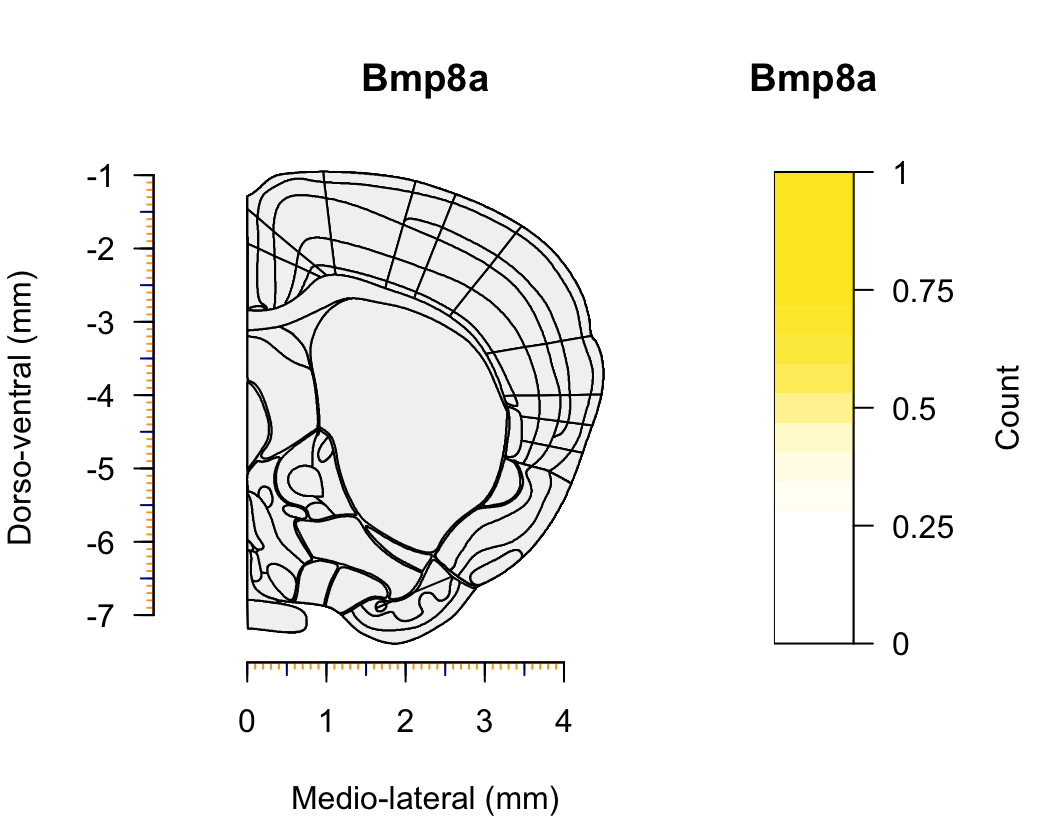
\includegraphics{wholebrain-bookdown_files/figure-latex/unnamed-chunk-16-10.pdf}

\begin{verbatim}
## Bmp8a
##  -----
##  Average number of Bmp8a transcripts detected:
##  CPu : M = 0 ( SD = 0 ) molecules 
##  SS : M = 0 ( SD = 0 ) molecules
##  -----
## 
##  Welch Two Sample t-test
## 
## data:  CP and SS
## t = NaN, df = NaN, p-value = NA
## alternative hypothesis: true difference in means is not equal to 0
## 95 percent confidence interval:
##  NaN NaN
## sample estimates:
## mean of x mean of y 
##         0         0
\end{verbatim}

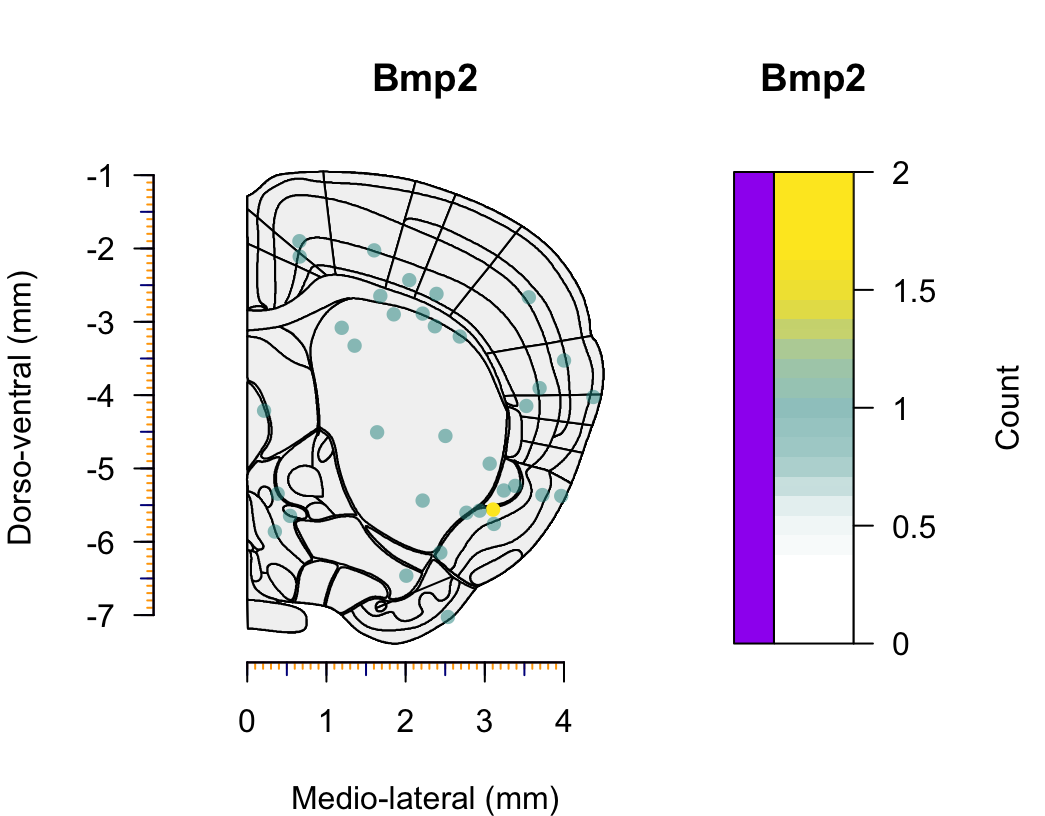
\includegraphics{wholebrain-bookdown_files/figure-latex/unnamed-chunk-16-11.pdf}

\begin{verbatim}
## Bmp2
##  -----
##  Average number of Bmp2 transcripts detected:
##  CPu : M = 0.08 ( SD = 0.27 ) molecules 
##  SS : M = 0.04 ( SD = 0.2 ) molecules
##  -----
## 
##  Welch Two Sample t-test
## 
## data:  CP and SS
## t = 1.1883, df = 213.44, p-value = 0.236
## alternative hypothesis: true difference in means is not equal to 0
## 95 percent confidence interval:
##  -0.02389638  0.09644173
## sample estimates:
##  mean of x  mean of y 
## 0.07692308 0.04065041
\end{verbatim}

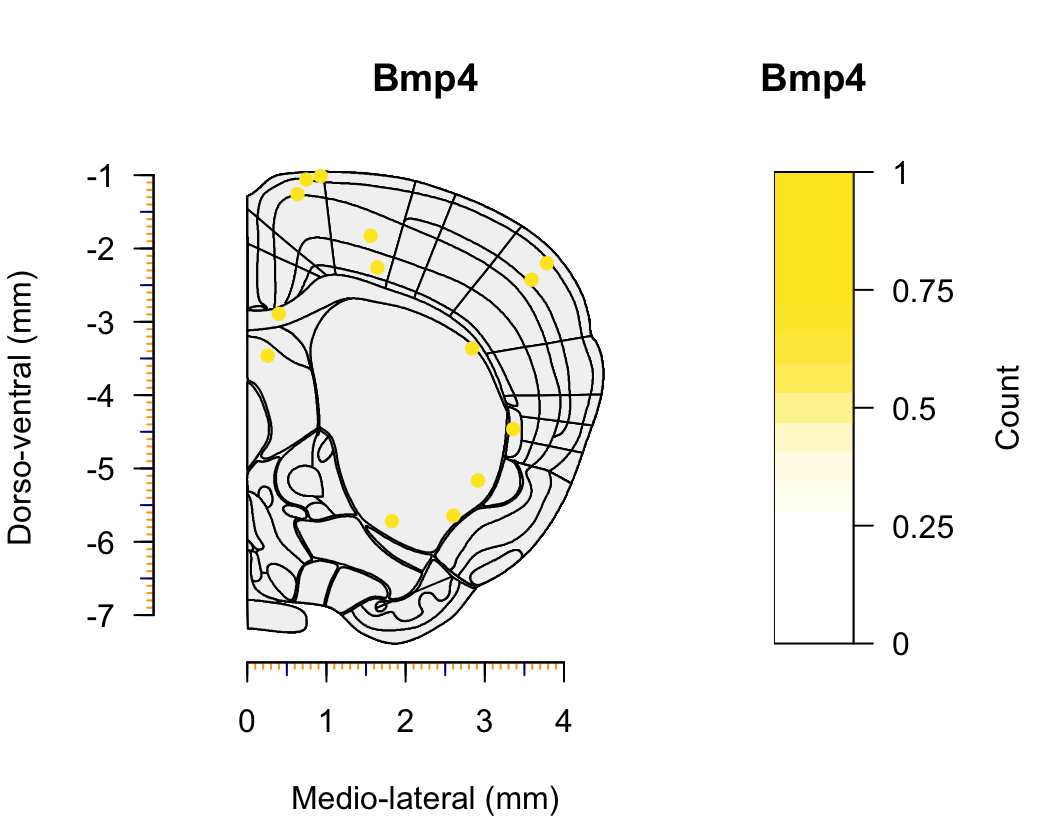
\includegraphics{wholebrain-bookdown_files/figure-latex/unnamed-chunk-16-12.pdf}

\begin{verbatim}
## Bmp4
##  -----
##  Average number of Bmp4 transcripts detected:
##  CPu : M = 0.03 ( SD = 0.18 ) molecules 
##  SS : M = 0.02 ( SD = 0.13 ) molecules
##  -----
## 
##  Welch Two Sample t-test
## 
## data:  CP and SS
## t = 0.87924, df = 205.93, p-value = 0.3803
## alternative hypothesis: true difference in means is not equal to 0
## 95 percent confidence interval:
##  -0.02227249  0.05812823
## sample estimates:
##  mean of x  mean of y 
## 0.03418803 0.01626016
\end{verbatim}

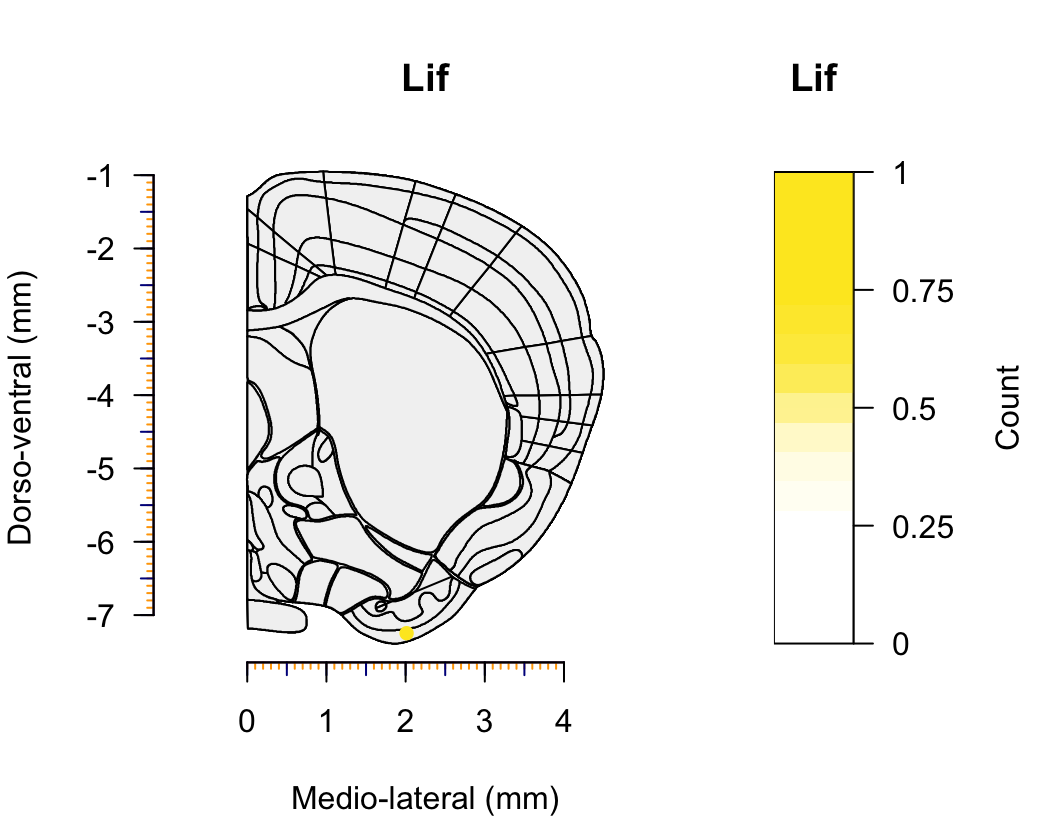
\includegraphics{wholebrain-bookdown_files/figure-latex/unnamed-chunk-16-13.pdf}

\begin{verbatim}
## Lif
##  -----
##  Average number of Lif transcripts detected:
##  CPu : M = 0 ( SD = 0 ) molecules 
##  SS : M = 0 ( SD = 0 ) molecules
##  -----
## 
##  Welch Two Sample t-test
## 
## data:  CP and SS
## t = NaN, df = NaN, p-value = NA
## alternative hypothesis: true difference in means is not equal to 0
## 95 percent confidence interval:
##  NaN NaN
## sample estimates:
## mean of x mean of y 
##         0         0
\end{verbatim}

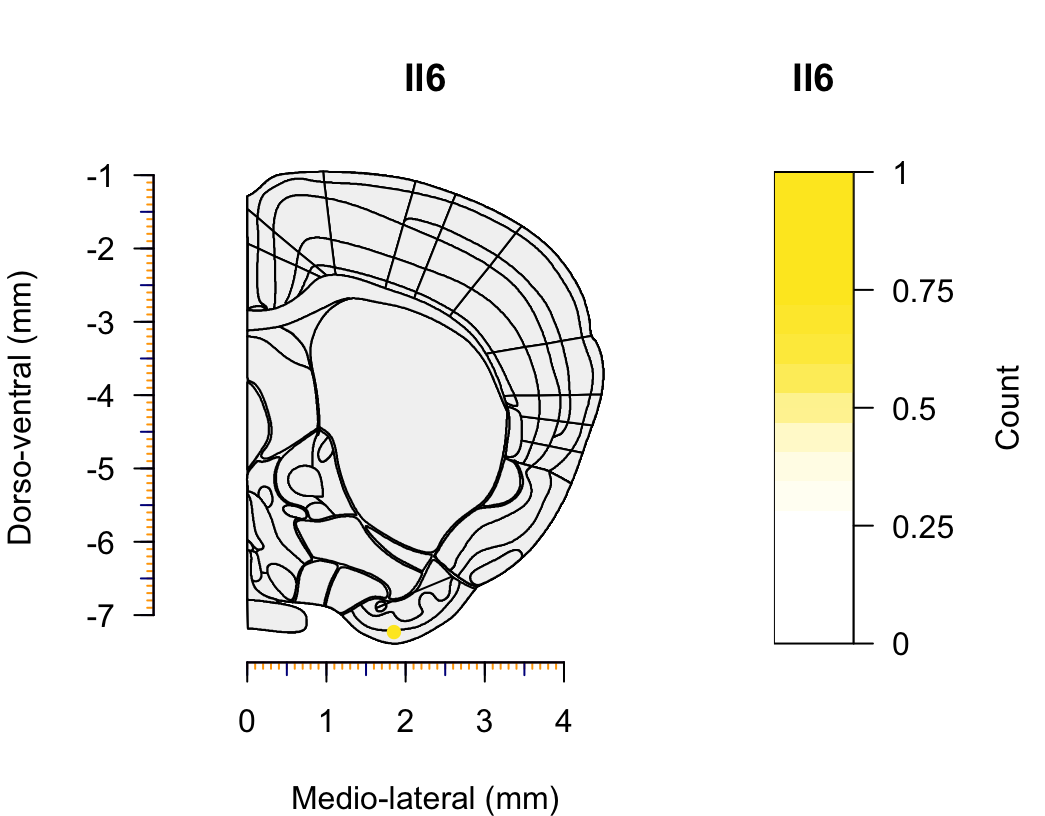
\includegraphics{wholebrain-bookdown_files/figure-latex/unnamed-chunk-16-14.pdf}

\begin{verbatim}
## Il6
##  -----
##  Average number of Il6 transcripts detected:
##  CPu : M = 0 ( SD = 0 ) molecules 
##  SS : M = 0 ( SD = 0 ) molecules
##  -----
## 
##  Welch Two Sample t-test
## 
## data:  CP and SS
## t = NaN, df = NaN, p-value = NA
## alternative hypothesis: true difference in means is not equal to 0
## 95 percent confidence interval:
##  NaN NaN
## sample estimates:
## mean of x mean of y 
##         0         0
\end{verbatim}

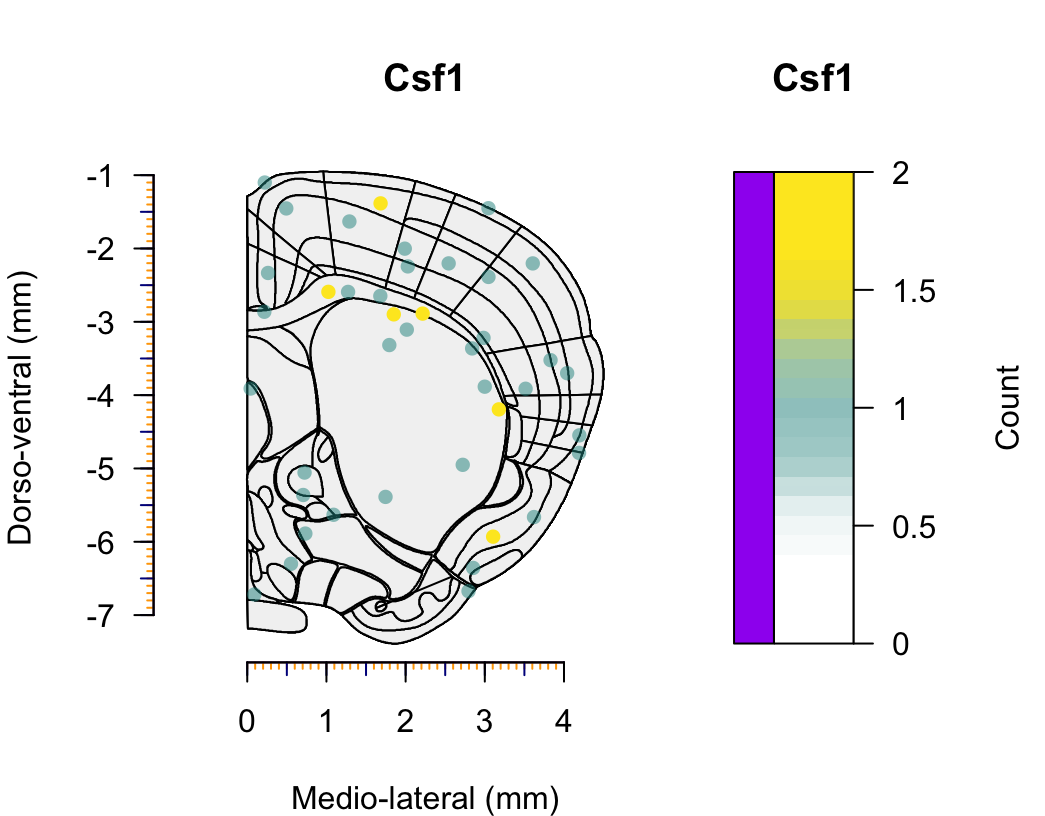
\includegraphics{wholebrain-bookdown_files/figure-latex/unnamed-chunk-16-15.pdf}

\begin{verbatim}
## Csf1
##  -----
##  Average number of Csf1 transcripts detected:
##  CPu : M = 0.09 ( SD = 0.34 ) molecules 
##  SS : M = 0.08 ( SD = 0.27 ) molecules
##  -----
## 
##  Welch Two Sample t-test
## 
## data:  CP and SS
## t = 0.10486, df = 223.93, p-value = 0.9166
## alternative hypothesis: true difference in means is not equal to 0
## 95 percent confidence interval:
##  -0.07418047  0.08251902
## sample estimates:
##  mean of x  mean of y 
## 0.08547009 0.08130081
\end{verbatim}

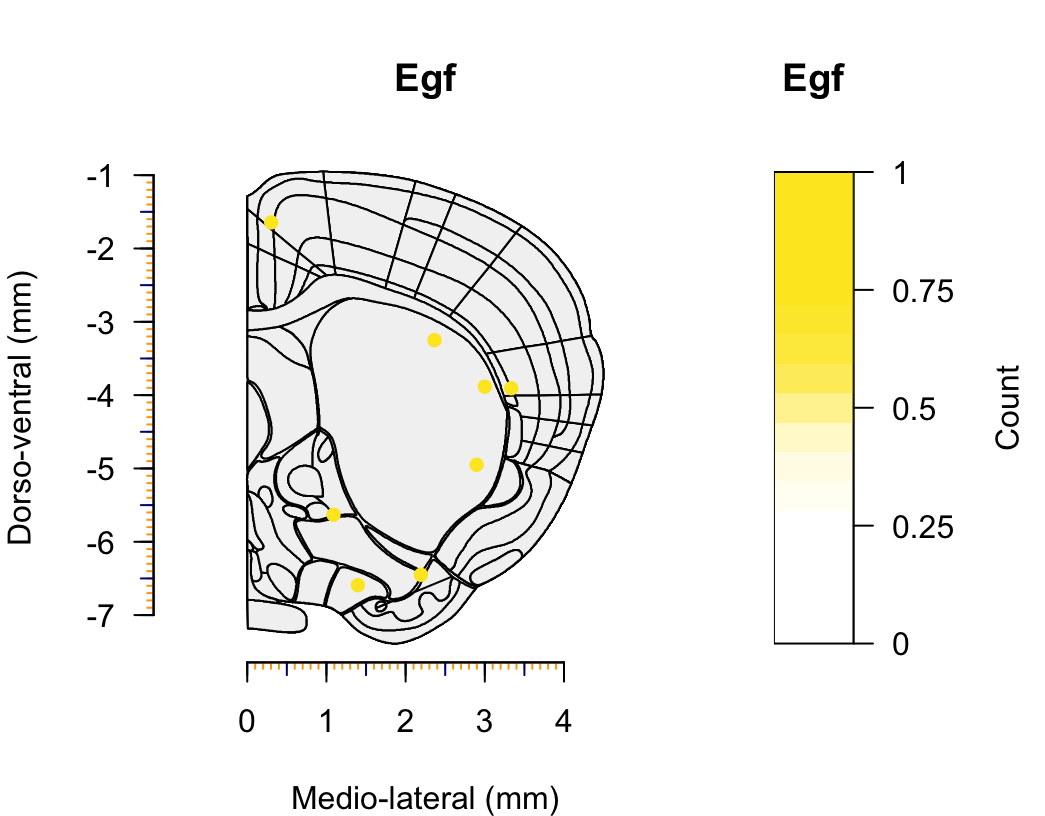
\includegraphics{wholebrain-bookdown_files/figure-latex/unnamed-chunk-16-16.pdf}

\begin{verbatim}
## Egf
##  -----
##  Average number of Egf transcripts detected:
##  CPu : M = 0.03 ( SD = 0.16 ) molecules 
##  SS : M = 0.01 ( SD = 0.09 ) molecules
##  -----
## 
##  Welch Two Sample t-test
## 
## data:  CP and SS
## t = 1.0437, df = 181.84, p-value = 0.298
## alternative hypothesis: true difference in means is not equal to 0
## 95 percent confidence interval:
##  -0.01559204  0.05061392
## sample estimates:
##   mean of x   mean of y 
## 0.025641026 0.008130081
\end{verbatim}

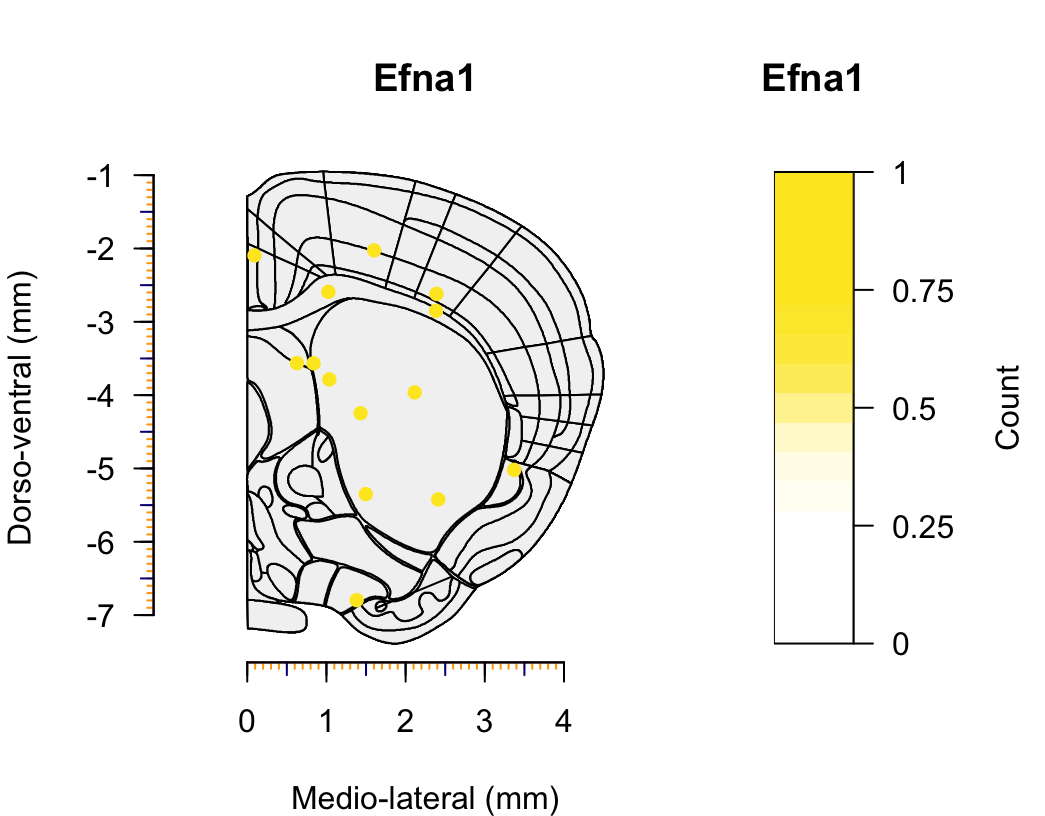
\includegraphics{wholebrain-bookdown_files/figure-latex/unnamed-chunk-16-17.pdf}

\begin{verbatim}
## Efna1
##  -----
##  Average number of Efna1 transcripts detected:
##  CPu : M = 0.05 ( SD = 0.22 ) molecules 
##  SS : M = 0.01 ( SD = 0.09 ) molecules
##  -----
## 
##  Welch Two Sample t-test
## 
## data:  CP and SS
## t = 1.9584, df = 151.86, p-value = 0.05202
## alternative hypothesis: true difference in means is not equal to 0
## 95 percent confidence interval:
##  -0.0003815429  0.0866854829
## sample estimates:
##   mean of x   mean of y 
## 0.051282051 0.008130081
\end{verbatim}

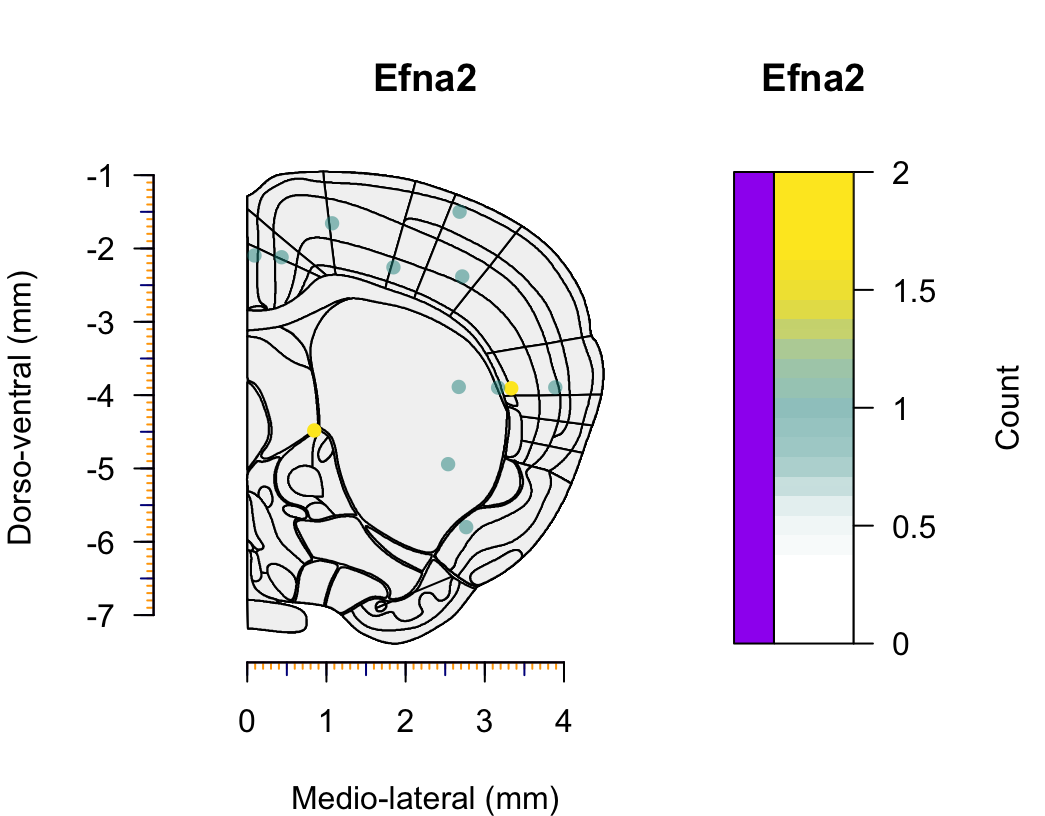
\includegraphics{wholebrain-bookdown_files/figure-latex/unnamed-chunk-16-18.pdf}

\begin{verbatim}
## Efna2
##  -----
##  Average number of Efna2 transcripts detected:
##  CPu : M = 0.02 ( SD = 0.13 ) molecules 
##  SS : M = 0.05 ( SD = 0.25 ) molecules
##  -----
## 
##  Welch Two Sample t-test
## 
## data:  CP and SS
## t = -1.2348, df = 185.04, p-value = 0.2185
## alternative hypothesis: true difference in means is not equal to 0
## 95 percent confidence interval:
##  -0.08231115  0.01893820
## sample estimates:
##  mean of x  mean of y 
## 0.01709402 0.04878049
\end{verbatim}

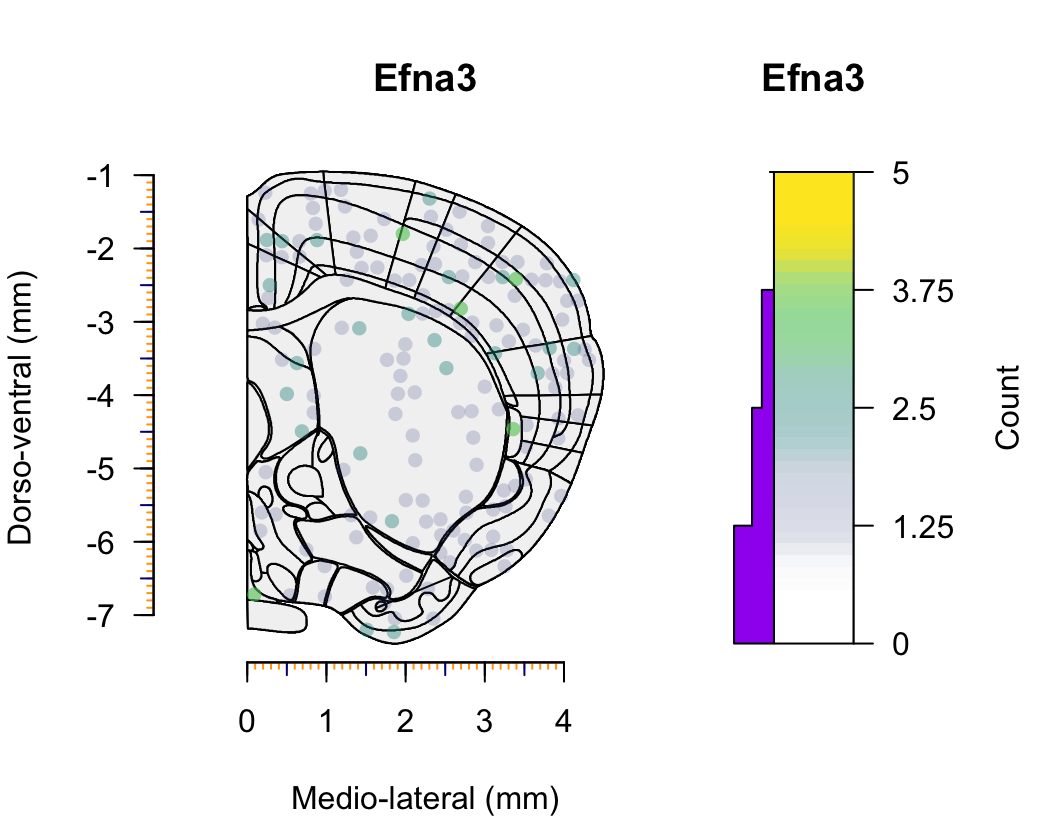
\includegraphics{wholebrain-bookdown_files/figure-latex/unnamed-chunk-16-19.pdf}

\begin{verbatim}
## Efna3        █▬█ █ ▀█▀ MARKER FOR SOMATOSENSORY!
##  -----
##  Average number of Efna3 transcripts detected:
##  CPu : M = 0.32 ( SD = 0.57 ) molecules 
##  SS : M = 0.51 ( SD = 0.73 ) molecules
##  -----
## 
##  Welch Two Sample t-test
## 
## data:  CP and SS
## t = -2.226, df = 229.54, p-value = 0.02699
## alternative hypothesis: true difference in means is not equal to 0
## 95 percent confidence interval:
##  -0.35329814 -0.02151946
## sample estimates:
## mean of x mean of y 
## 0.3247863 0.5121951
\end{verbatim}

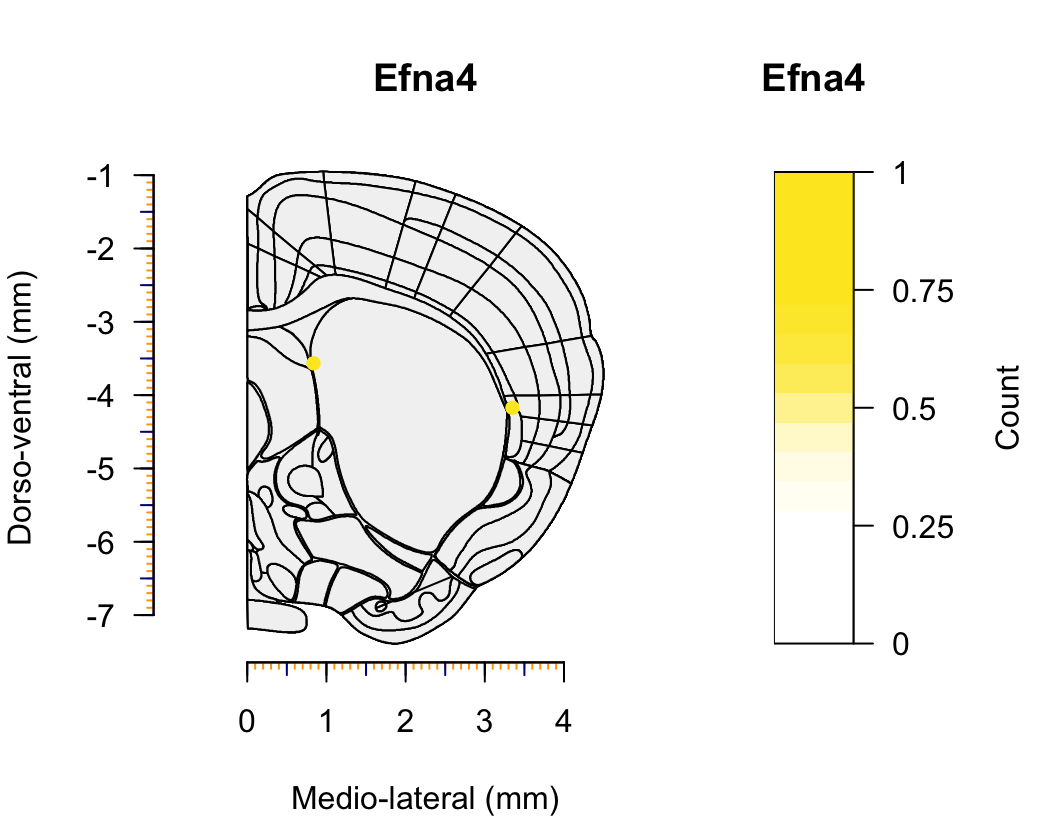
\includegraphics{wholebrain-bookdown_files/figure-latex/unnamed-chunk-16-20.pdf}

\begin{verbatim}
## Efna4
##  -----
##  Average number of Efna4 transcripts detected:
##  CPu : M = 0.01 ( SD = 0.09 ) molecules 
##  SS : M = 0 ( SD = 0 ) molecules
##  -----
## 
##  Welch Two Sample t-test
## 
## data:  CP and SS
## t = 1, df = 116, p-value = 0.3194
## alternative hypothesis: true difference in means is not equal to 0
## 95 percent confidence interval:
##  -0.008381419  0.025475436
## sample estimates:
##   mean of x   mean of y 
## 0.008547009 0.000000000
\end{verbatim}

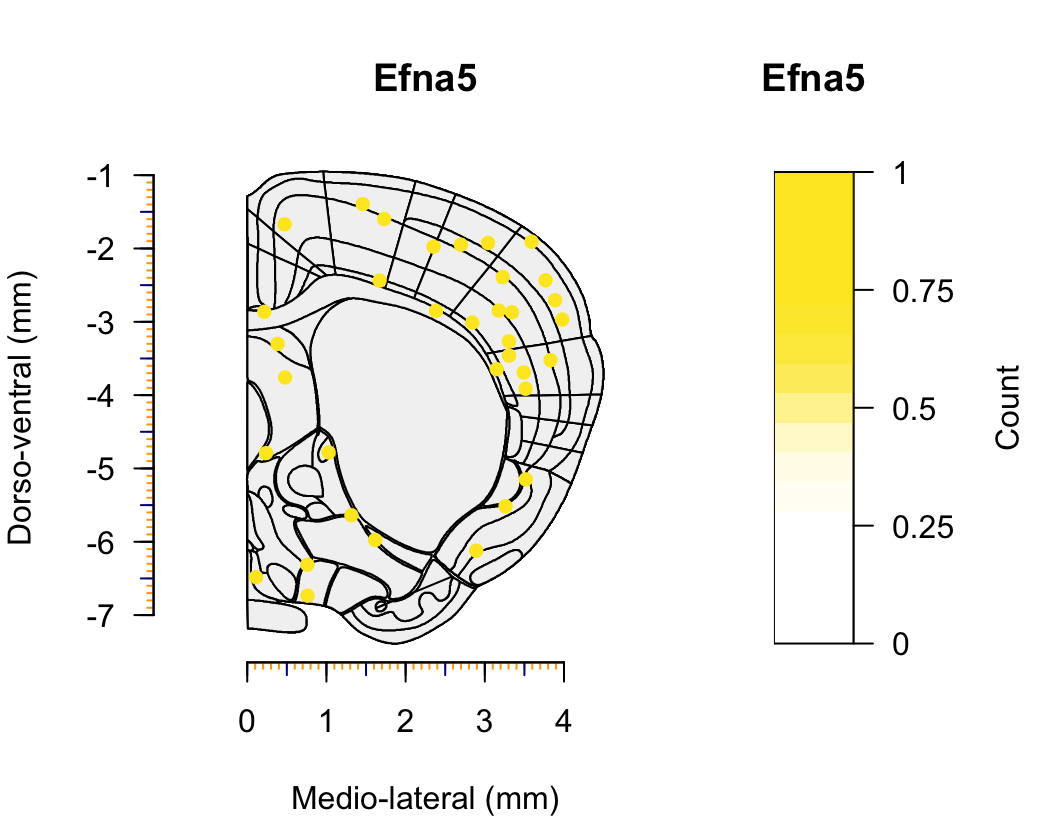
\includegraphics{wholebrain-bookdown_files/figure-latex/unnamed-chunk-16-21.pdf}

\begin{verbatim}
## Efna5        █▬█ █ ▀█▀ MARKER FOR SOMATOSENSORY!
##  -----
##  Average number of Efna5 transcripts detected:
##  CPu : M = 0 ( SD = 0 ) molecules 
##  SS : M = 0.14 ( SD = 0.35 ) molecules
##  -----
## 
##  Welch Two Sample t-test
## 
## data:  CP and SS
## t = -4.4234, df = 122, p-value = 2.125e-05
## alternative hypothesis: true difference in means is not equal to 0
## 95 percent confidence interval:
##  -0.2000657 -0.0763571
## sample estimates:
## mean of x mean of y 
## 0.0000000 0.1382114
\end{verbatim}

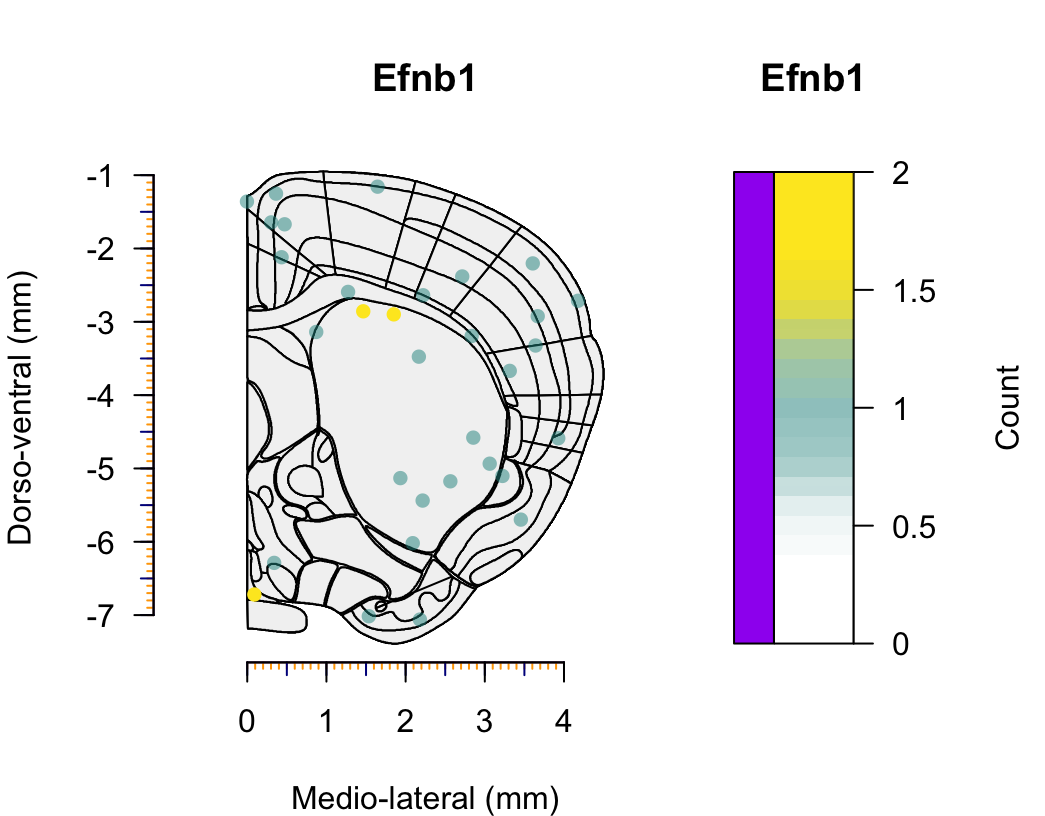
\includegraphics{wholebrain-bookdown_files/figure-latex/unnamed-chunk-16-22.pdf}

\begin{verbatim}
## Efnb1
##  -----
##  Average number of Efnb1 transcripts detected:
##  CPu : M = 0.1 ( SD = 0.36 ) molecules 
##  SS : M = 0.06 ( SD = 0.23 ) molecules
##  -----
## 
##  Welch Two Sample t-test
## 
## data:  CP and SS
## t = 1.1679, df = 197.98, p-value = 0.2443
## alternative hypothesis: true difference in means is not equal to 0
## 95 percent confidence interval:
##  -0.03143564  0.12274270
## sample estimates:
##  mean of x  mean of y 
## 0.10256410 0.05691057
\end{verbatim}

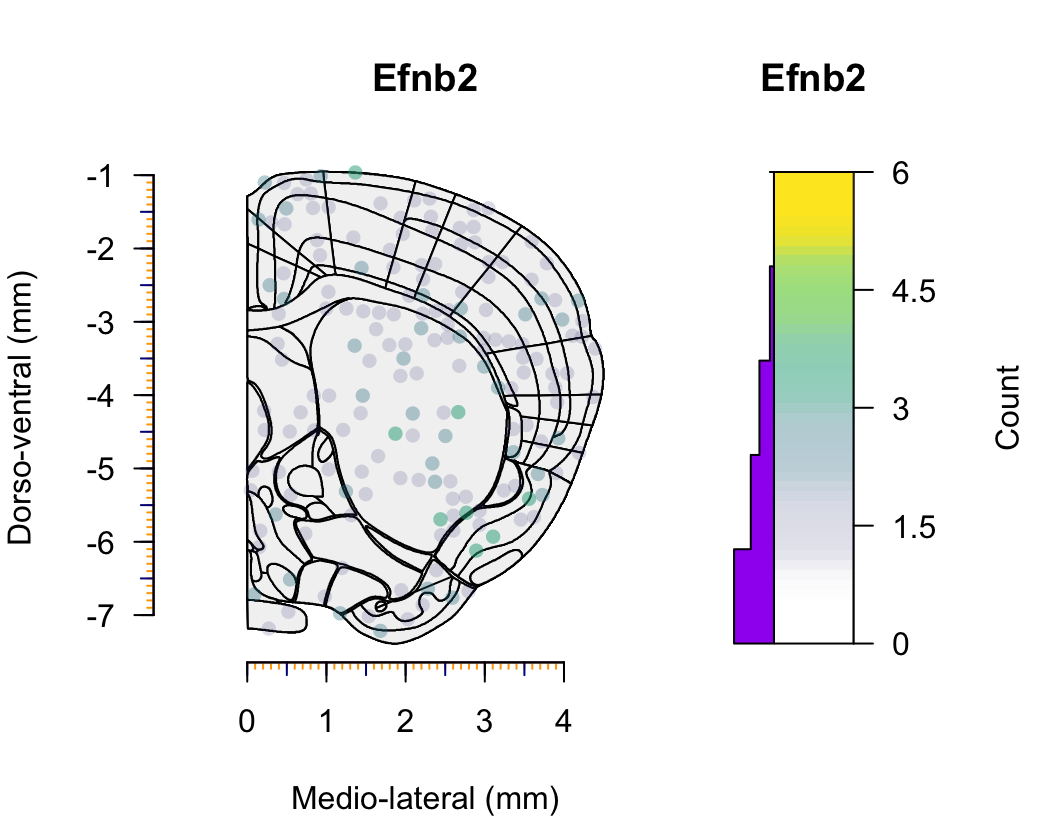
\includegraphics{wholebrain-bookdown_files/figure-latex/unnamed-chunk-16-23.pdf}

\begin{verbatim}
## Efnb2
##  -----
##  Average number of Efnb2 transcripts detected:
##  CPu : M = 0.49 ( SD = 0.76 ) molecules 
##  SS : M = 0.43 ( SD = 0.59 ) molecules
##  -----
## 
##  Welch Two Sample t-test
## 
## data:  CP and SS
## t = 0.63881, df = 218.17, p-value = 0.5236
## alternative hypothesis: true difference in means is not equal to 0
## 95 percent confidence interval:
##  -0.1173703  0.2299407
## sample estimates:
## mean of x mean of y 
## 0.4871795 0.4308943
\end{verbatim}

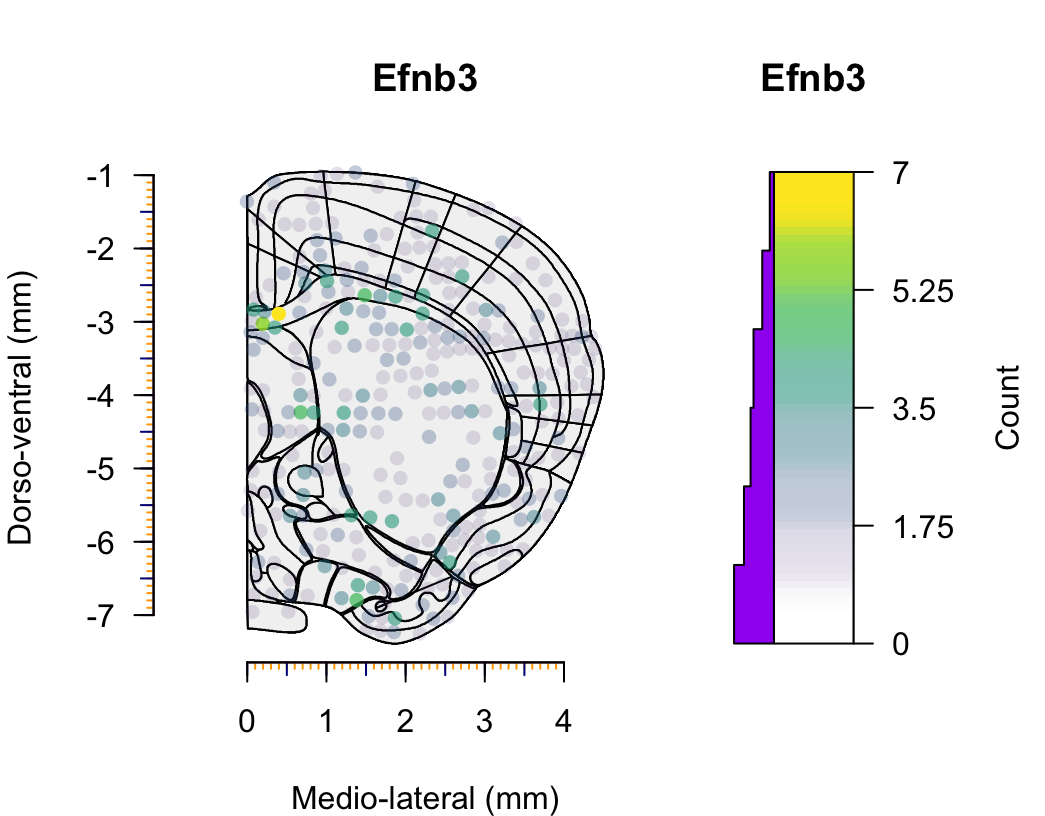
\includegraphics{wholebrain-bookdown_files/figure-latex/unnamed-chunk-16-24.pdf}

\begin{verbatim}
## Efnb3        █▬█ █ ▀█▀ MARKER FOR CAUDATE PUTAMEN!
##  -----
##  Average number of Efnb3 transcripts detected:
##  CPu : M = 1.12 ( SD = 1.12 ) molecules 
##  SS : M = 0.68 ( SD = 0.85 ) molecules
##  -----
## 
##  Welch Two Sample t-test
## 
## data:  CP and SS
## t = 3.3958, df = 217, p-value = 0.0008138
## alternative hypothesis: true difference in means is not equal to 0
## 95 percent confidence interval:
##  0.1832461 0.6902165
## sample estimates:
## mean of x mean of y 
## 1.1196581 0.6829268
\end{verbatim}

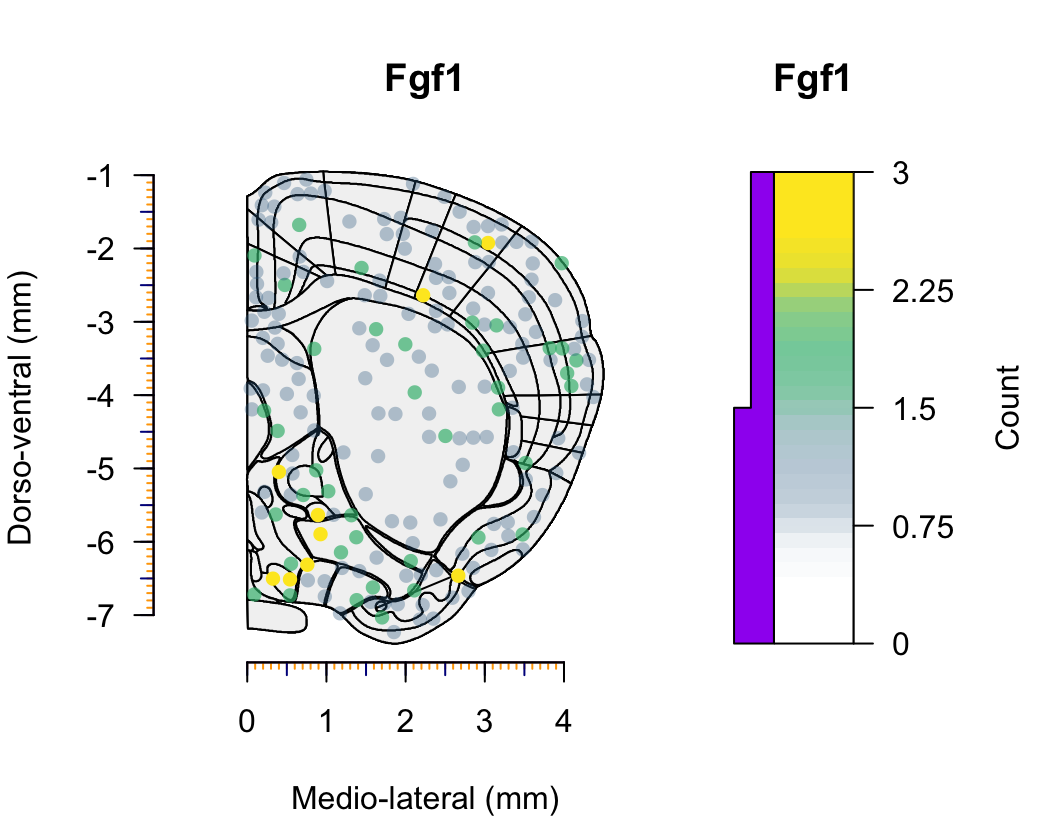
\includegraphics{wholebrain-bookdown_files/figure-latex/unnamed-chunk-16-25.pdf}

\begin{verbatim}
## Fgf1        █▬█ █ ▀█▀ MARKER FOR SOMATOSENSORY!
##  -----
##  Average number of Fgf1 transcripts detected:
##  CPu : M = 0.32 ( SD = 0.57 ) molecules 
##  SS : M = 0.49 ( SD = 0.71 ) molecules
##  -----
## 
##  Welch Two Sample t-test
## 
## data:  CP and SS
## t = -1.9737, df = 231.96, p-value = 0.0496
## alternative hypothesis: true difference in means is not equal to 0
## 95 percent confidence interval:
##  -0.3257498750 -0.0002872315
## sample estimates:
## mean of x mean of y 
## 0.3247863 0.4878049
\end{verbatim}

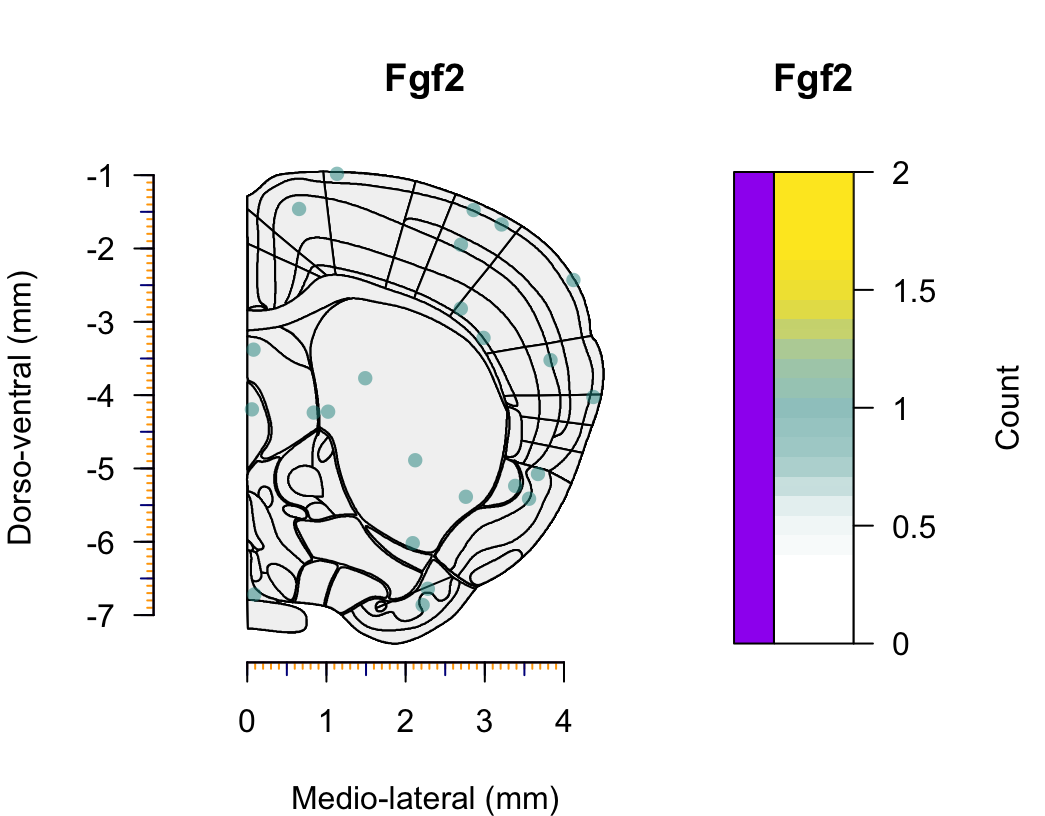
\includegraphics{wholebrain-bookdown_files/figure-latex/unnamed-chunk-16-26.pdf}

\begin{verbatim}
## Fgf2
##  -----
##  Average number of Fgf2 transcripts detected:
##  CPu : M = 0.04 ( SD = 0.2 ) molecules 
##  SS : M = 0.06 ( SD = 0.23 ) molecules
##  -----
## 
##  Welch Two Sample t-test
## 
## data:  CP and SS
## t = -0.50352, df = 236.3, p-value = 0.6151
## alternative hypothesis: true difference in means is not equal to 0
## 95 percent confidence interval:
##  -0.06963856  0.04128750
## sample estimates:
##  mean of x  mean of y 
## 0.04273504 0.05691057
\end{verbatim}

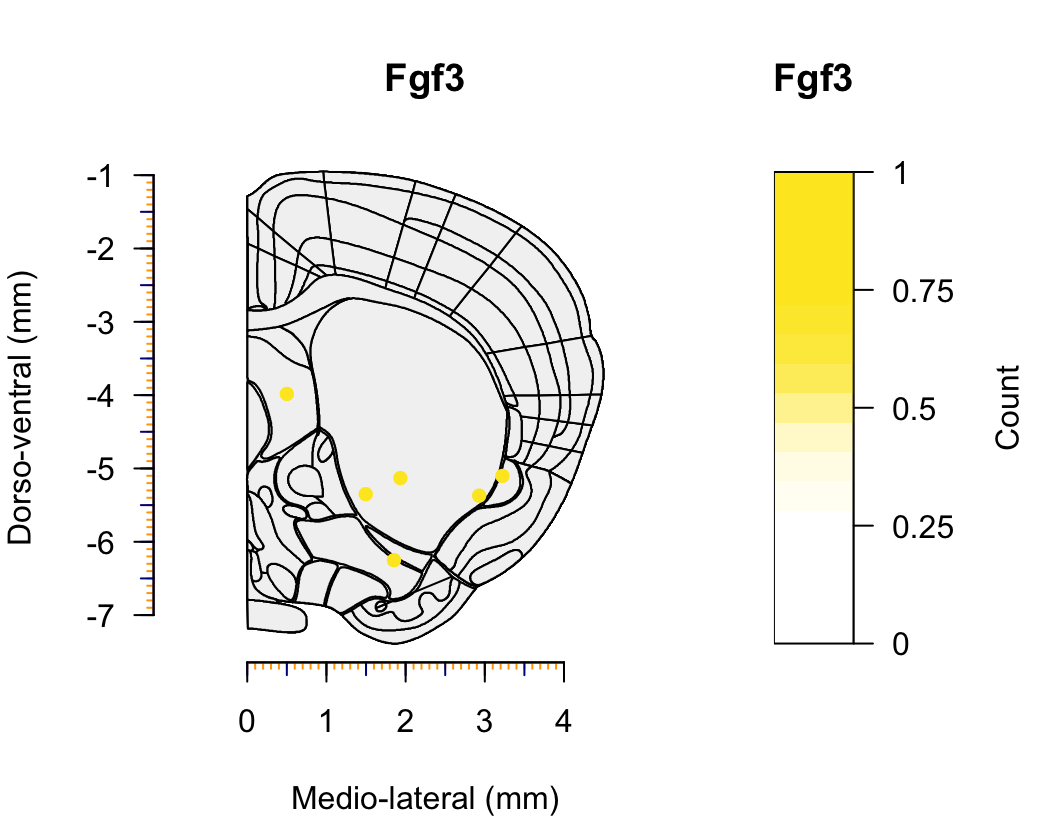
\includegraphics{wholebrain-bookdown_files/figure-latex/unnamed-chunk-16-27.pdf}

\begin{verbatim}
## Fgf3
##  -----
##  Average number of Fgf3 transcripts detected:
##  CPu : M = 0.03 ( SD = 0.16 ) molecules 
##  SS : M = 0 ( SD = 0 ) molecules
##  -----
## 
##  Welch Two Sample t-test
## 
## data:  CP and SS
## t = 1.7472, df = 116, p-value = 0.08325
## alternative hypothesis: true difference in means is not equal to 0
## 95 percent confidence interval:
##  -0.003426005  0.054708057
## sample estimates:
##  mean of x  mean of y 
## 0.02564103 0.00000000
\end{verbatim}

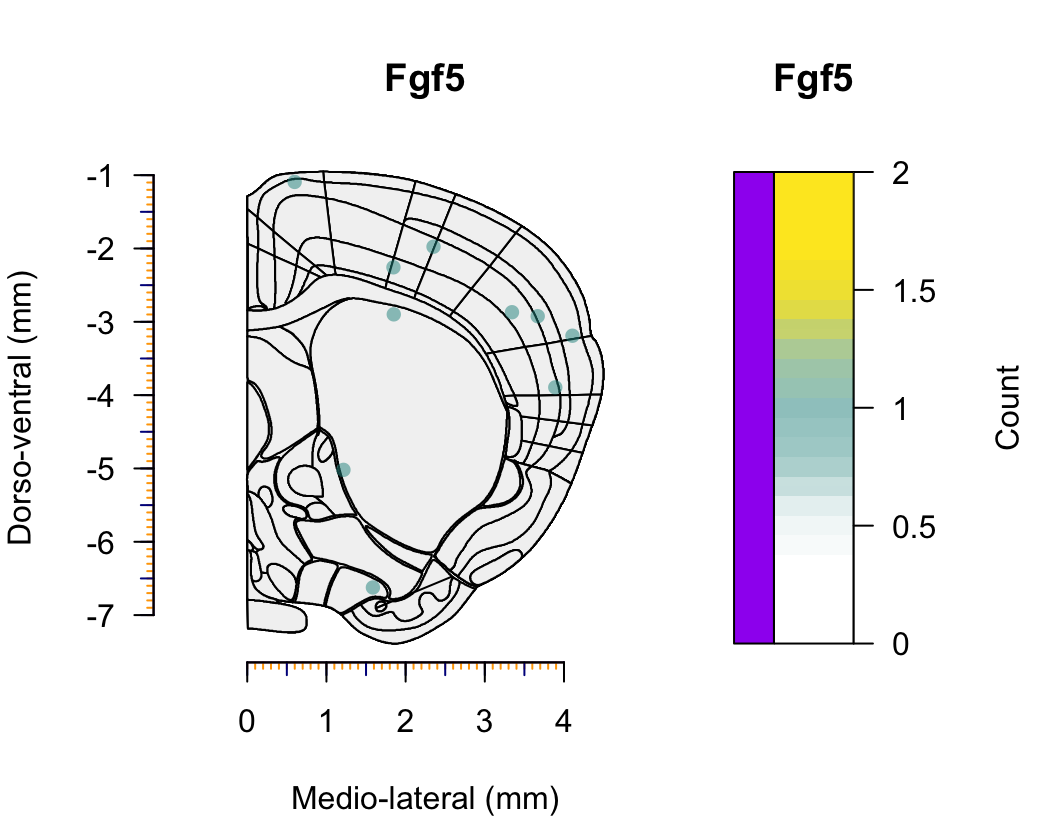
\includegraphics{wholebrain-bookdown_files/figure-latex/unnamed-chunk-16-28.pdf}

\begin{verbatim}
## Fgf5
##  -----
##  Average number of Fgf5 transcripts detected:
##  CPu : M = 0.02 ( SD = 0.13 ) molecules 
##  SS : M = 0.05 ( SD = 0.22 ) molecules
##  -----
## 
##  Welch Two Sample t-test
## 
## data:  CP and SS
## t = -1.3827, df = 201.83, p-value = 0.1683
## alternative hypothesis: true difference in means is not equal to 0
## 95 percent confidence interval:
##  -0.07687349  0.01350055
## sample estimates:
##  mean of x  mean of y 
## 0.01709402 0.04878049
\end{verbatim}

\includegraphics{wholebrain-bookdown_files/figure-latex/unnamed-chunk-16-29.pdf}

\begin{verbatim}
## Fgf7
##  -----
##  Average number of Fgf7 transcripts detected:
##  CPu : M = 0.01 ( SD = 0.09 ) molecules 
##  SS : M = 0 ( SD = 0 ) molecules
##  -----
## 
##  Welch Two Sample t-test
## 
## data:  CP and SS
## t = 1, df = 116, p-value = 0.3194
## alternative hypothesis: true difference in means is not equal to 0
## 95 percent confidence interval:
##  -0.008381419  0.025475436
## sample estimates:
##   mean of x   mean of y 
## 0.008547009 0.000000000
\end{verbatim}

\includegraphics{wholebrain-bookdown_files/figure-latex/unnamed-chunk-16-30.pdf}

\begin{verbatim}
## Fgf8
##  -----
##  Average number of Fgf8 transcripts detected:
##  CPu : M = 0 ( SD = 0 ) molecules 
##  SS : M = 0 ( SD = 0 ) molecules
##  -----
## 
##  Welch Two Sample t-test
## 
## data:  CP and SS
## t = NaN, df = NaN, p-value = NA
## alternative hypothesis: true difference in means is not equal to 0
## 95 percent confidence interval:
##  NaN NaN
## sample estimates:
## mean of x mean of y 
##         0         0
\end{verbatim}

\includegraphics{wholebrain-bookdown_files/figure-latex/unnamed-chunk-16-31.pdf}

\begin{verbatim}
## Fgf9
##  -----
##  Average number of Fgf9 transcripts detected:
##  CPu : M = 0.23 ( SD = 0.46 ) molecules 
##  SS : M = 0.28 ( SD = 0.56 ) molecules
##  -----
## 
##  Welch Two Sample t-test
## 
## data:  CP and SS
## t = -0.68845, df = 233.11, p-value = 0.4919
## alternative hypothesis: true difference in means is not equal to 0
## 95 percent confidence interval:
##  -0.17630326  0.08499619
## sample estimates:
## mean of x mean of y 
## 0.2307692 0.2764228
\end{verbatim}

\includegraphics{wholebrain-bookdown_files/figure-latex/unnamed-chunk-16-32.pdf}

\begin{verbatim}
## Fgf10
##  -----
##  Average number of Fgf10 transcripts detected:
##  CPu : M = 0.01 ( SD = 0.09 ) molecules 
##  SS : M = 0.04 ( SD = 0.24 ) molecules
##  -----
## 
##  Welch Two Sample t-test
## 
## data:  CP and SS
## t = -1.3998, df = 160.15, p-value = 0.1635
## alternative hypothesis: true difference in means is not equal to 0
## 95 percent confidence interval:
##  -0.07739627  0.01318947
## sample estimates:
##   mean of x   mean of y 
## 0.008547009 0.040650407
\end{verbatim}

\includegraphics{wholebrain-bookdown_files/figure-latex/unnamed-chunk-16-33.pdf}

\begin{verbatim}
## Fgf11
##  -----
##  Average number of Fgf11 transcripts detected:
##  CPu : M = 0.19 ( SD = 0.49 ) molecules 
##  SS : M = 0.12 ( SD = 0.33 ) molecules
##  -----
## 
##  Welch Two Sample t-test
## 
## data:  CP and SS
## t = 1.2207, df = 201.39, p-value = 0.2236
## alternative hypothesis: true difference in means is not equal to 0
## 95 percent confidence interval:
##  -0.04066287  0.17282881
## sample estimates:
## mean of x mean of y 
## 0.1880342 0.1219512
\end{verbatim}

\includegraphics{wholebrain-bookdown_files/figure-latex/unnamed-chunk-16-34.pdf}

\begin{verbatim}
## Fgf12        █▬█ █ ▀█▀ MARKER FOR SOMATOSENSORY!
##  -----
##  Average number of Fgf12 transcripts detected:
##  CPu : M = 0.93 ( SD = 0.94 ) molecules 
##  SS : M = 1.99 ( SD = 1.58 ) molecules
##  -----
## 
##  Welch Two Sample t-test
## 
## data:  CP and SS
## t = -6.359, df = 199.82, p-value = 1.354e-09
## alternative hypothesis: true difference in means is not equal to 0
## 95 percent confidence interval:
##  -1.3890276 -0.7314643
## sample estimates:
## mean of x mean of y 
## 0.9316239 1.9918699
\end{verbatim}

\includegraphics{wholebrain-bookdown_files/figure-latex/unnamed-chunk-16-35.pdf}

\begin{verbatim}
## Fgf13        █▬█ █ ▀█▀ MARKER FOR SOMATOSENSORY!
##  -----
##  Average number of Fgf13 transcripts detected:
##  CPu : M = 1.26 ( SD = 1.27 ) molecules 
##  SS : M = 2.02 ( SD = 1.55 ) molecules
##  -----
## 
##  Welch Two Sample t-test
## 
## data:  CP and SS
## t = -4.2025, df = 233.17, p-value = 3.762e-05
## alternative hypothesis: true difference in means is not equal to 0
## 95 percent confidence interval:
##  -1.1280204 -0.4079396
## sample estimates:
## mean of x mean of y 
##   1.25641   2.02439
\end{verbatim}

\includegraphics{wholebrain-bookdown_files/figure-latex/unnamed-chunk-16-36.pdf}

\begin{verbatim}
## Fgf14
##  -----
##  Average number of Fgf14 transcripts detected:
##  CPu : M = 0.3 ( SD = 0.61 ) molecules 
##  SS : M = 0.37 ( SD = 0.63 ) molecules
##  -----
## 
##  Welch Two Sample t-test
## 
## data:  CP and SS
## t = -0.83594, df = 237.98, p-value = 0.404
## alternative hypothesis: true difference in means is not equal to 0
## 95 percent confidence interval:
##  -0.22391406  0.09049735
## sample estimates:
## mean of x mean of y 
## 0.2991453 0.3658537
\end{verbatim}

\includegraphics{wholebrain-bookdown_files/figure-latex/unnamed-chunk-16-37.pdf}

\begin{verbatim}
## Fgf16
##  -----
##  Average number of Fgf16 transcripts detected:
##  CPu : M = 0.02 ( SD = 0.13 ) molecules 
##  SS : M = 0 ( SD = 0 ) molecules
##  -----
## 
##  Welch Two Sample t-test
## 
## data:  CP and SS
## t = 1.4203, df = 116, p-value = 0.1582
## alternative hypothesis: true difference in means is not equal to 0
## 95 percent confidence interval:
##  -0.00674298  0.04093101
## sample estimates:
##  mean of x  mean of y 
## 0.01709402 0.00000000
\end{verbatim}

\includegraphics{wholebrain-bookdown_files/figure-latex/unnamed-chunk-16-38.pdf}

\begin{verbatim}
## Fgf17
##  -----
##  Average number of Fgf17 transcripts detected:
##  CPu : M = 0 ( SD = 0 ) molecules 
##  SS : M = 0 ( SD = 0 ) molecules
##  -----
## 
##  Welch Two Sample t-test
## 
## data:  CP and SS
## t = NaN, df = NaN, p-value = NA
## alternative hypothesis: true difference in means is not equal to 0
## 95 percent confidence interval:
##  NaN NaN
## sample estimates:
## mean of x mean of y 
##         0         0
\end{verbatim}

\includegraphics{wholebrain-bookdown_files/figure-latex/unnamed-chunk-16-39.pdf}

\begin{verbatim}
## Fgf18
##  -----
##  Average number of Fgf18 transcripts detected:
##  CPu : M = 0 ( SD = 0 ) molecules 
##  SS : M = 0 ( SD = 0 ) molecules
##  -----
## 
##  Welch Two Sample t-test
## 
## data:  CP and SS
## t = NaN, df = NaN, p-value = NA
## alternative hypothesis: true difference in means is not equal to 0
## 95 percent confidence interval:
##  NaN NaN
## sample estimates:
## mean of x mean of y 
##         0         0
\end{verbatim}

\includegraphics{wholebrain-bookdown_files/figure-latex/unnamed-chunk-16-40.pdf}

\begin{verbatim}
## Fgf22
##  -----
##  Average number of Fgf22 transcripts detected:
##  CPu : M = 0 ( SD = 0 ) molecules 
##  SS : M = 0.01 ( SD = 0.09 ) molecules
##  -----
## 
##  Welch Two Sample t-test
## 
## data:  CP and SS
## t = -1, df = 122, p-value = 0.3193
## alternative hypothesis: true difference in means is not equal to 0
## 95 percent confidence interval:
##  -0.024224389  0.007964227
## sample estimates:
##   mean of x   mean of y 
## 0.000000000 0.008130081
\end{verbatim}

\includegraphics{wholebrain-bookdown_files/figure-latex/unnamed-chunk-16-41.pdf}

\begin{verbatim}
## Gdnf
##  -----
##  Average number of Gdnf transcripts detected:
##  CPu : M = 0.03 ( SD = 0.22 ) molecules 
##  SS : M = 0 ( SD = 0 ) molecules
##  -----
## 
##  Welch Two Sample t-test
## 
## data:  CP and SS
## t = 1.6449, df = 116, p-value = 0.1027
## alternative hypothesis: true difference in means is not equal to 0
## 95 percent confidence interval:
##  -0.006979009  0.075355078
## sample estimates:
##  mean of x  mean of y 
## 0.03418803 0.00000000
\end{verbatim}

\includegraphics{wholebrain-bookdown_files/figure-latex/unnamed-chunk-16-42.pdf}

\begin{verbatim}
## Nrtn        █▬█ █ ▀█▀ MARKER FOR CAUDATE PUTAMEN!
##  -----
##  Average number of Nrtn transcripts detected:
##  CPu : M = 0.31 ( SD = 0.69 ) molecules 
##  SS : M = 0.08 ( SD = 0.27 ) molecules
##  -----
## 
##  Welch Two Sample t-test
## 
## data:  CP and SS
## t = 3.3168, df = 150.48, p-value = 0.001142
## alternative hypothesis: true difference in means is not equal to 0
## 95 percent confidence interval:
##  0.09152566 0.36125732
## sample estimates:
##  mean of x  mean of y 
## 0.30769231 0.08130081
\end{verbatim}

\includegraphics{wholebrain-bookdown_files/figure-latex/unnamed-chunk-16-43.pdf}

\begin{verbatim}
## Artn
##  -----
##  Average number of Artn transcripts detected:
##  CPu : M = 0 ( SD = 0 ) molecules 
##  SS : M = 0 ( SD = 0 ) molecules
##  -----
## 
##  Welch Two Sample t-test
## 
## data:  CP and SS
## t = NaN, df = NaN, p-value = NA
## alternative hypothesis: true difference in means is not equal to 0
## 95 percent confidence interval:
##  NaN NaN
## sample estimates:
## mean of x mean of y 
##         0         0
\end{verbatim}

\includegraphics{wholebrain-bookdown_files/figure-latex/unnamed-chunk-16-44.pdf}

\begin{verbatim}
## Gdf9
##  -----
##  Average number of Gdf9 transcripts detected:
##  CPu : M = 0 ( SD = 0 ) molecules 
##  SS : M = 0.01 ( SD = 0.09 ) molecules
##  -----
## 
##  Welch Two Sample t-test
## 
## data:  CP and SS
## t = -1, df = 122, p-value = 0.3193
## alternative hypothesis: true difference in means is not equal to 0
## 95 percent confidence interval:
##  -0.024224389  0.007964227
## sample estimates:
##   mean of x   mean of y 
## 0.000000000 0.008130081
\end{verbatim}

\includegraphics{wholebrain-bookdown_files/figure-latex/unnamed-chunk-16-45.pdf}

\begin{verbatim}
## Hgf
##  -----
##  Average number of Hgf transcripts detected:
##  CPu : M = 0.01 ( SD = 0.09 ) molecules 
##  SS : M = 0.01 ( SD = 0.09 ) molecules
##  -----
## 
##  Welch Two Sample t-test
## 
## data:  CP and SS
## t = 0.035344, df = 236.66, p-value = 0.9718
## alternative hypothesis: true difference in means is not equal to 0
## 95 percent confidence interval:
##  -0.02282198  0.02365583
## sample estimates:
##   mean of x   mean of y 
## 0.008547009 0.008130081
\end{verbatim}

\includegraphics{wholebrain-bookdown_files/figure-latex/unnamed-chunk-16-46.pdf}

\begin{verbatim}
## Hdgf
##  -----
##  Average number of Hdgf transcripts detected:
##  CPu : M = 1.03 ( SD = 0.97 ) molecules 
##  SS : M = 1.16 ( SD = 1.09 ) molecules
##  -----
## 
##  Welch Two Sample t-test
## 
## data:  CP and SS
## t = -1.0303, df = 236.95, p-value = 0.3039
## alternative hypothesis: true difference in means is not equal to 0
## 95 percent confidence interval:
##  -0.3988450  0.1249238
## sample estimates:
## mean of x mean of y 
##  1.025641  1.162602
\end{verbatim}

\includegraphics{wholebrain-bookdown_files/figure-latex/unnamed-chunk-16-47.pdf}

\begin{verbatim}
## Igf1
##  -----
##  Average number of Igf1 transcripts detected:
##  CPu : M = 0.02 ( SD = 0.13 ) molecules 
##  SS : M = 0.02 ( SD = 0.15 ) molecules
##  -----
## 
##  Welch Two Sample t-test
## 
## data:  CP and SS
## t = -0.39576, df = 234.48, p-value = 0.6926
## alternative hypothesis: true difference in means is not equal to 0
## 95 percent confidence interval:
##  -0.04361765  0.02902520
## sample estimates:
##  mean of x  mean of y 
## 0.01709402 0.02439024
\end{verbatim}

\includegraphics{wholebrain-bookdown_files/figure-latex/unnamed-chunk-16-48.pdf}

\begin{verbatim}
## Igf2
##  -----
##  Average number of Igf2 transcripts detected:
##  CPu : M = 0.22 ( SD = 0.56 ) molecules 
##  SS : M = 0.22 ( SD = 0.63 ) molecules
##  -----
## 
##  Welch Two Sample t-test
## 
## data:  CP and SS
## t = 0.035165, df = 236.63, p-value = 0.972
## alternative hypothesis: true difference in means is not equal to 0
## 95 percent confidence interval:
##  -0.1491126  0.1545326
## sample estimates:
## mean of x mean of y 
## 0.2222222 0.2195122
\end{verbatim}

\includegraphics{wholebrain-bookdown_files/figure-latex/unnamed-chunk-16-49.pdf}

\begin{verbatim}
## Il1a
##  -----
##  Average number of Il1a transcripts detected:
##  CPu : M = 0.01 ( SD = 0.09 ) molecules 
##  SS : M = 0 ( SD = 0 ) molecules
##  -----
## 
##  Welch Two Sample t-test
## 
## data:  CP and SS
## t = 1, df = 116, p-value = 0.3194
## alternative hypothesis: true difference in means is not equal to 0
## 95 percent confidence interval:
##  -0.008381419  0.025475436
## sample estimates:
##   mean of x   mean of y 
## 0.008547009 0.000000000
\end{verbatim}

\includegraphics{wholebrain-bookdown_files/figure-latex/unnamed-chunk-16-50.pdf}

\begin{verbatim}
## Il1b
##  -----
##  Average number of Il1b transcripts detected:
##  CPu : M = 0 ( SD = 0 ) molecules 
##  SS : M = 0.01 ( SD = 0.09 ) molecules
##  -----
## 
##  Welch Two Sample t-test
## 
## data:  CP and SS
## t = -1, df = 122, p-value = 0.3193
## alternative hypothesis: true difference in means is not equal to 0
## 95 percent confidence interval:
##  -0.024224389  0.007964227
## sample estimates:
##   mean of x   mean of y 
## 0.000000000 0.008130081
\end{verbatim}

\includegraphics{wholebrain-bookdown_files/figure-latex/unnamed-chunk-16-51.pdf}

\begin{verbatim}
## Il2
##  -----
##  Average number of Il2 transcripts detected:
##  CPu : M = 0.17 ( SD = 0.4 ) molecules 
##  SS : M = 0.24 ( SD = 0.58 ) molecules
##  -----
## 
##  Welch Two Sample t-test
## 
## data:  CP and SS
## t = -1.1422, df = 217.89, p-value = 0.2546
## alternative hypothesis: true difference in means is not equal to 0
## 95 percent confidence interval:
##  -0.19885697  0.05293243
## sample estimates:
## mean of x mean of y 
## 0.1709402 0.2439024
\end{verbatim}

\includegraphics{wholebrain-bookdown_files/figure-latex/unnamed-chunk-16-52.pdf}

\begin{verbatim}
## Il4
##  -----
##  Average number of Il4 transcripts detected:
##  CPu : M = 0 ( SD = 0 ) molecules 
##  SS : M = 0.01 ( SD = 0.09 ) molecules
##  -----
## 
##  Welch Two Sample t-test
## 
## data:  CP and SS
## t = -1, df = 122, p-value = 0.3193
## alternative hypothesis: true difference in means is not equal to 0
## 95 percent confidence interval:
##  -0.024224389  0.007964227
## sample estimates:
##   mean of x   mean of y 
## 0.000000000 0.008130081
\end{verbatim}

\includegraphics{wholebrain-bookdown_files/figure-latex/unnamed-chunk-16-53.pdf}

\begin{verbatim}
## Il5
##  -----
##  Average number of Il5 transcripts detected:
##  CPu : M = 0 ( SD = 0 ) molecules 
##  SS : M = 0.01 ( SD = 0.09 ) molecules
##  -----
## 
##  Welch Two Sample t-test
## 
## data:  CP and SS
## t = -1, df = 122, p-value = 0.3193
## alternative hypothesis: true difference in means is not equal to 0
## 95 percent confidence interval:
##  -0.024224389  0.007964227
## sample estimates:
##   mean of x   mean of y 
## 0.000000000 0.008130081
\end{verbatim}

\includegraphics{wholebrain-bookdown_files/figure-latex/unnamed-chunk-16-54.pdf}

\begin{verbatim}
## Il6
##  -----
##  Average number of Il6 transcripts detected:
##  CPu : M = 0 ( SD = 0 ) molecules 
##  SS : M = 0 ( SD = 0 ) molecules
##  -----
## 
##  Welch Two Sample t-test
## 
## data:  CP and SS
## t = NaN, df = NaN, p-value = NA
## alternative hypothesis: true difference in means is not equal to 0
## 95 percent confidence interval:
##  NaN NaN
## sample estimates:
## mean of x mean of y 
##         0         0
\end{verbatim}

\includegraphics{wholebrain-bookdown_files/figure-latex/unnamed-chunk-16-55.pdf}

\begin{verbatim}
## Nrg1
##  -----
##  Average number of Nrg1 transcripts detected:
##  CPu : M = 0.07 ( SD = 0.25 ) molecules 
##  SS : M = 0.11 ( SD = 0.33 ) molecules
##  -----
## 
##  Welch Two Sample t-test
## 
## data:  CP and SS
## t = -0.97752, df = 226.9, p-value = 0.3294
## alternative hypothesis: true difference in means is not equal to 0
## 95 percent confidence interval:
##  -0.11253401  0.03790404
## sample estimates:
##  mean of x  mean of y 
## 0.06837607 0.10569106
\end{verbatim}

\includegraphics{wholebrain-bookdown_files/figure-latex/unnamed-chunk-16-56.pdf}

\begin{verbatim}
## Nrg2
##  -----
##  Average number of Nrg2 transcripts detected:
##  CPu : M = 0.05 ( SD = 0.22 ) molecules 
##  SS : M = 0.07 ( SD = 0.26 ) molecules
##  -----
## 
##  Welch Two Sample t-test
## 
## data:  CP and SS
## t = -0.70089, df = 234.91, p-value = 0.4841
## alternative hypothesis: true difference in means is not equal to 0
## 95 percent confidence interval:
##  -0.08341464  0.03963728
## sample estimates:
##  mean of x  mean of y 
## 0.05128205 0.07317073
\end{verbatim}

\includegraphics{wholebrain-bookdown_files/figure-latex/unnamed-chunk-16-57.pdf}

\begin{verbatim}
## Nrg3
##  -----
##  Average number of Nrg3 transcripts detected:
##  CPu : M = 0.15 ( SD = 0.38 ) molecules 
##  SS : M = 0.24 ( SD = 0.51 ) molecules
##  -----
## 
##  Welch Two Sample t-test
## 
## data:  CP and SS
## t = -1.5605, df = 223.98, p-value = 0.12
## alternative hypothesis: true difference in means is not equal to 0
## 95 percent confidence interval:
##  -0.20472212  0.02377569
## sample estimates:
## mean of x mean of y 
## 0.1452991 0.2357724
\end{verbatim}

\includegraphics{wholebrain-bookdown_files/figure-latex/unnamed-chunk-16-58.pdf}

\begin{verbatim}
## Nrg4
##  -----
##  Average number of Nrg4 transcripts detected:
##  CPu : M = 0.02 ( SD = 0.13 ) molecules 
##  SS : M = 0.04 ( SD = 0.2 ) molecules
##  -----
## 
##  Welch Two Sample t-test
## 
## data:  CP and SS
## t = -1.093, df = 211.86, p-value = 0.2756
## alternative hypothesis: true difference in means is not equal to 0
## 95 percent confidence interval:
##  -0.06604067  0.01892789
## sample estimates:
##  mean of x  mean of y 
## 0.01709402 0.04065041
\end{verbatim}

\includegraphics{wholebrain-bookdown_files/figure-latex/unnamed-chunk-16-59.pdf}

\begin{verbatim}
## Bdnf        █▬█ █ ▀█▀ MARKER FOR SOMATOSENSORY!
##  -----
##  Average number of Bdnf transcripts detected:
##  CPu : M = 0.12 ( SD = 0.35 ) molecules 
##  SS : M = 0.36 ( SD = 0.63 ) molecules
##  -----
## 
##  Welch Two Sample t-test
## 
## data:  CP and SS
## t = -3.6425, df = 193.32, p-value = 0.0003467
## alternative hypothesis: true difference in means is not equal to 0
## 95 percent confidence interval:
##  -0.3669696 -0.1091613
## sample estimates:
## mean of x mean of y 
## 0.1196581 0.3577236
\end{verbatim}

\includegraphics{wholebrain-bookdown_files/figure-latex/unnamed-chunk-16-60.pdf}

\begin{verbatim}
## Ngf
##  -----
##  Average number of Ngf transcripts detected:
##  CPu : M = 0.01 ( SD = 0.09 ) molecules 
##  SS : M = 0 ( SD = 0 ) molecules
##  -----
## 
##  Welch Two Sample t-test
## 
## data:  CP and SS
## t = 1, df = 116, p-value = 0.3194
## alternative hypothesis: true difference in means is not equal to 0
## 95 percent confidence interval:
##  -0.008381419  0.025475436
## sample estimates:
##   mean of x   mean of y 
## 0.008547009 0.000000000
\end{verbatim}

\includegraphics{wholebrain-bookdown_files/figure-latex/unnamed-chunk-16-61.pdf}

\begin{verbatim}
## Ntf3
##  -----
##  Average number of Ntf3 transcripts detected:
##  CPu : M = 0.01 ( SD = 0.09 ) molecules 
##  SS : M = 0 ( SD = 0 ) molecules
##  -----
## 
##  Welch Two Sample t-test
## 
## data:  CP and SS
## t = 1, df = 116, p-value = 0.3194
## alternative hypothesis: true difference in means is not equal to 0
## 95 percent confidence interval:
##  -0.008381419  0.025475436
## sample estimates:
##   mean of x   mean of y 
## 0.008547009 0.000000000
\end{verbatim}

\includegraphics{wholebrain-bookdown_files/figure-latex/unnamed-chunk-16-62.pdf}

\begin{verbatim}
## Pgf
##  -----
##  Average number of Pgf transcripts detected:
##  CPu : M = 0.04 ( SD = 0.2 ) molecules 
##  SS : M = 0.02 ( SD = 0.13 ) molecules
##  -----
## 
##  Welch Two Sample t-test
## 
## data:  CP and SS
## t = 1.2037, df = 192.93, p-value = 0.2302
## alternative hypothesis: true difference in means is not equal to 0
## 95 percent confidence interval:
##  -0.01690641  0.06985617
## sample estimates:
##  mean of x  mean of y 
## 0.04273504 0.01626016
\end{verbatim}

\includegraphics{wholebrain-bookdown_files/figure-latex/unnamed-chunk-16-63.pdf}

\begin{verbatim}
## Pdgfa
##  -----
##  Average number of Pdgfa transcripts detected:
##  CPu : M = 0.57 ( SD = 0.85 ) molecules 
##  SS : M = 0.62 ( SD = 0.85 ) molecules
##  -----
## 
##  Welch Two Sample t-test
## 
## data:  CP and SS
## t = -0.41007, df = 237.41, p-value = 0.6821
## alternative hypothesis: true difference in means is not equal to 0
## 95 percent confidence interval:
##  -0.2625587  0.1720855
## sample estimates:
## mean of x mean of y 
## 0.5726496 0.6178862
\end{verbatim}

\includegraphics{wholebrain-bookdown_files/figure-latex/unnamed-chunk-16-64.pdf}

\begin{verbatim}
## Pdgfb
##  -----
##  Average number of Pdgfb transcripts detected:
##  CPu : M = 0.13 ( SD = 0.36 ) molecules 
##  SS : M = 0.2 ( SD = 0.44 ) molecules
##  -----
## 
##  Welch Two Sample t-test
## 
## data:  CP and SS
## t = -1.443, df = 232.53, p-value = 0.1504
## alternative hypothesis: true difference in means is not equal to 0
## 95 percent confidence interval:
##  -0.17751393  0.02742012
## sample estimates:
## mean of x mean of y 
## 0.1282051 0.2032520
\end{verbatim}

\includegraphics{wholebrain-bookdown_files/figure-latex/unnamed-chunk-16-65.pdf}

\begin{verbatim}
## Rnls
##  -----
##  Average number of Rnls transcripts detected:
##  CPu : M = 0.03 ( SD = 0.16 ) molecules 
##  SS : M = 0.02 ( SD = 0.2 ) molecules
##  -----
## 
##  Welch Two Sample t-test
## 
## data:  CP and SS
## t = 0.053642, df = 230.32, p-value = 0.9573
## alternative hypothesis: true difference in means is not equal to 0
## 95 percent confidence interval:
##  -0.04469182  0.04719339
## sample estimates:
##  mean of x  mean of y 
## 0.02564103 0.02439024
\end{verbatim}

\includegraphics{wholebrain-bookdown_files/figure-latex/unnamed-chunk-16-66.pdf}

\begin{verbatim}
## Tpo
##  -----
##  Average number of Tpo transcripts detected:
##  CPu : M = 0 ( SD = 0 ) molecules 
##  SS : M = 0 ( SD = 0 ) molecules
##  -----
## 
##  Welch Two Sample t-test
## 
## data:  CP and SS
## t = NaN, df = NaN, p-value = NA
## alternative hypothesis: true difference in means is not equal to 0
## 95 percent confidence interval:
##  NaN NaN
## sample estimates:
## mean of x mean of y 
##         0         0
\end{verbatim}

\includegraphics{wholebrain-bookdown_files/figure-latex/unnamed-chunk-16-67.pdf}

\begin{verbatim}
## Tgfa        █▬█ █ ▀█▀ MARKER FOR CAUDATE PUTAMEN!
##  -----
##  Average number of Tgfa transcripts detected:
##  CPu : M = 0.45 ( SD = 0.62 ) molecules 
##  SS : M = 0.13 ( SD = 0.36 ) molecules
##  -----
## 
##  Welch Two Sample t-test
## 
## data:  CP and SS
## t = 4.8815, df = 184.19, p-value = 2.274e-06
## alternative hypothesis: true difference in means is not equal to 0
## 95 percent confidence interval:
##  0.1924007 0.4534196
## sample estimates:
## mean of x mean of y 
## 0.4529915 0.1300813
\end{verbatim}

\includegraphics{wholebrain-bookdown_files/figure-latex/unnamed-chunk-16-68.pdf}

\begin{verbatim}
## Tgfb1
##  -----
##  Average number of Tgfb1 transcripts detected:
##  CPu : M = 0.04 ( SD = 0.2 ) molecules 
##  SS : M = 0.01 ( SD = 0.09 ) molecules
##  -----
## 
##  Welch Two Sample t-test
## 
## data:  CP and SS
## t = 1.691, df = 158.27, p-value = 0.0928
## alternative hypothesis: true difference in means is not equal to 0
## 95 percent confidence interval:
##  -0.005812046  0.075021969
## sample estimates:
##   mean of x   mean of y 
## 0.042735043 0.008130081
\end{verbatim}

\includegraphics{wholebrain-bookdown_files/figure-latex/unnamed-chunk-16-69.pdf}

\begin{verbatim}
## Tgfb2
##  -----
##  Average number of Tgfb2 transcripts detected:
##  CPu : M = 0.06 ( SD = 0.27 ) molecules 
##  SS : M = 0.03 ( SD = 0.18 ) molecules
##  -----
## 
##  Welch Two Sample t-test
## 
## data:  CP and SS
## t = 0.91531, df = 198.52, p-value = 0.3611
## alternative hypothesis: true difference in means is not equal to 0
## 95 percent confidence interval:
##  -0.03152665  0.08614412
## sample estimates:
##  mean of x  mean of y 
## 0.05982906 0.03252033
\end{verbatim}

\includegraphics{wholebrain-bookdown_files/figure-latex/unnamed-chunk-16-70.pdf}

\begin{verbatim}
## Tgfb3
##  -----
##  Average number of Tgfb3 transcripts detected:
##  CPu : M = 0 ( SD = 0 ) molecules 
##  SS : M = 0.02 ( SD = 0.15 ) molecules
##  -----
## 
##  Welch Two Sample t-test
## 
## data:  CP and SS
## t = -1.7464, df = 122, p-value = 0.08325
## alternative hypothesis: true difference in means is not equal to 0
## 95 percent confidence interval:
##  -0.052036966  0.003256478
## sample estimates:
##  mean of x  mean of y 
## 0.00000000 0.02439024
\end{verbatim}

\includegraphics{wholebrain-bookdown_files/figure-latex/unnamed-chunk-16-71.pdf}

\begin{verbatim}
## Vegfa
##  -----
##  Average number of Vegfa transcripts detected:
##  CPu : M = 0.5 ( SD = 0.82 ) molecules 
##  SS : M = 0.5 ( SD = 0.73 ) molecules
##  -----
## 
##  Welch Two Sample t-test
## 
## data:  CP and SS
## t = 0.002084, df = 231.85, p-value = 0.9983
## alternative hypothesis: true difference in means is not equal to 0
## 95 percent confidence interval:
##  -0.1968806  0.1972975
## sample estimates:
## mean of x mean of y 
## 0.5042735 0.5040650
\end{verbatim}

\includegraphics{wholebrain-bookdown_files/figure-latex/unnamed-chunk-16-72.pdf}

\begin{verbatim}
## Vegfb        █▬█ █ ▀█▀ MARKER FOR SOMATOSENSORY!
##  -----
##  Average number of Vegfb transcripts detected:
##  CPu : M = 1.24 ( SD = 1.24 ) molecules 
##  SS : M = 1.59 ( SD = 1.42 ) molecules
##  -----
## 
##  Welch Two Sample t-test
## 
## data:  CP and SS
## t = -2.0644, df = 236.2, p-value = 0.04007
## alternative hypothesis: true difference in means is not equal to 0
## 95 percent confidence interval:
##  -0.69217742 -0.01618197
## sample estimates:
## mean of x mean of y 
##  1.239316  1.593496
\end{verbatim}

\includegraphics{wholebrain-bookdown_files/figure-latex/unnamed-chunk-16-73.pdf}

\begin{verbatim}
## Vegfc
##  -----
##  Average number of Vegfc transcripts detected:
##  CPu : M = 0 ( SD = 0 ) molecules 
##  SS : M = 0.02 ( SD = 0.13 ) molecules
##  -----
## 
##  Welch Two Sample t-test
## 
## data:  CP and SS
## t = -1.42, df = 122, p-value = 0.1581
## alternative hypothesis: true difference in means is not equal to 0
## 95 percent confidence interval:
##  -0.038927477  0.006407152
## sample estimates:
##  mean of x  mean of y 
## 0.00000000 0.01626016
\end{verbatim}

\includegraphics{wholebrain-bookdown_files/figure-latex/unnamed-chunk-16-74.pdf}

\begin{verbatim}
## Vegfd
##  -----
##  Average number of Vegfd transcripts detected:
##  CPu : M = 0.01 ( SD = 0.09 ) molecules 
##  SS : M = 0.02 ( SD = 0.13 ) molecules
##  -----
## 
##  Welch Two Sample t-test
## 
## data:  CP and SS
## t = -0.53981, df = 223.01, p-value = 0.5899
## alternative hypothesis: true difference in means is not equal to 0
## 95 percent confidence interval:
##  -0.03587111  0.02044481
## sample estimates:
##   mean of x   mean of y 
## 0.008547009 0.016260163
\end{verbatim}

\includegraphics{wholebrain-bookdown_files/figure-latex/unnamed-chunk-16-75.pdf}

\begin{verbatim}
## Wnt2
##  -----
##  Average number of Wnt2 transcripts detected:
##  CPu : M = 0.03 ( SD = 0.18 ) molecules 
##  SS : M = 0.06 ( SD = 0.23 ) molecules
##  -----
## 
##  Welch Two Sample t-test
## 
## data:  CP and SS
## t = -0.84414, df = 229.78, p-value = 0.3995
## alternative hypothesis: true difference in means is not equal to 0
## 95 percent confidence interval:
##  -0.07576027  0.03031520
## sample estimates:
##  mean of x  mean of y 
## 0.03418803 0.05691057
\end{verbatim}

\includegraphics{wholebrain-bookdown_files/figure-latex/unnamed-chunk-16-76.pdf}

\begin{verbatim}
## Wnt4        █▬█ █ ▀█▀ MARKER FOR SOMATOSENSORY!
##  -----
##  Average number of Wnt4 transcripts detected:
##  CPu : M = 0.01 ( SD = 0.09 ) molecules 
##  SS : M = 0.16 ( SD = 0.39 ) molecules
##  -----
## 
##  Welch Two Sample t-test
## 
## data:  CP and SS
## t = -4.2363, df = 136.19, p-value = 4.159e-05
## alternative hypothesis: true difference in means is not equal to 0
## 95 percent confidence interval:
##  -0.22596777 -0.08214146
## sample estimates:
##   mean of x   mean of y 
## 0.008547009 0.162601626
\end{verbatim}

\includegraphics{wholebrain-bookdown_files/figure-latex/unnamed-chunk-16-77.pdf}

\begin{verbatim}
## Wnt5a        █▬█ █ ▀█▀ MARKER FOR CAUDATE PUTAMEN!
##  -----
##  Average number of Wnt5a transcripts detected:
##  CPu : M = 0.09 ( SD = 0.32 ) molecules 
##  SS : M = 0.02 ( SD = 0.15 ) molecules
##  -----
## 
##  Welch Two Sample t-test
## 
## data:  CP and SS
## t = 2.1219, df = 165.31, p-value = 0.03533
## alternative hypothesis: true difference in means is not equal to 0
## 95 percent confidence interval:
##  0.004840102 0.134413598
## sample estimates:
##  mean of x  mean of y 
## 0.09401709 0.02439024
\end{verbatim}

\includegraphics{wholebrain-bookdown_files/figure-latex/unnamed-chunk-16-78.pdf}

\begin{verbatim}
## Wnt5b
##  -----
##  Average number of Wnt5b transcripts detected:
##  CPu : M = 0 ( SD = 0 ) molecules 
##  SS : M = 0.01 ( SD = 0.09 ) molecules
##  -----
## 
##  Welch Two Sample t-test
## 
## data:  CP and SS
## t = -1, df = 122, p-value = 0.3193
## alternative hypothesis: true difference in means is not equal to 0
## 95 percent confidence interval:
##  -0.024224389  0.007964227
## sample estimates:
##   mean of x   mean of y 
## 0.000000000 0.008130081
\end{verbatim}

\includegraphics{wholebrain-bookdown_files/figure-latex/unnamed-chunk-16-79.pdf}

\begin{verbatim}
## Wnt6
##  -----
##  Average number of Wnt6 transcripts detected:
##  CPu : M = 0.01 ( SD = 0.09 ) molecules 
##  SS : M = 0.01 ( SD = 0.09 ) molecules
##  -----
## 
##  Welch Two Sample t-test
## 
## data:  CP and SS
## t = 0.035344, df = 236.66, p-value = 0.9718
## alternative hypothesis: true difference in means is not equal to 0
## 95 percent confidence interval:
##  -0.02282198  0.02365583
## sample estimates:
##   mean of x   mean of y 
## 0.008547009 0.008130081
\end{verbatim}

\includegraphics{wholebrain-bookdown_files/figure-latex/unnamed-chunk-16-80.pdf}

\begin{verbatim}
## Wnt7a
##  -----
##  Average number of Wnt7a transcripts detected:
##  CPu : M = 0.1 ( SD = 0.33 ) molecules 
##  SS : M = 0.05 ( SD = 0.22 ) molecules
##  -----
## 
##  Welch Two Sample t-test
## 
## data:  CP and SS
## t = 1.4797, df = 197.98, p-value = 0.1405
## alternative hypothesis: true difference in means is not equal to 0
## 95 percent confidence interval:
##  -0.01789558  0.12546281
## sample estimates:
##  mean of x  mean of y 
## 0.10256410 0.04878049
\end{verbatim}

\includegraphics{wholebrain-bookdown_files/figure-latex/unnamed-chunk-16-81.pdf}

\begin{verbatim}
## Wnt7b
##  -----
##  Average number of Wnt7b transcripts detected:
##  CPu : M = 0.15 ( SD = 0.4 ) molecules 
##  SS : M = 0.19 ( SD = 0.47 ) molecules
##  -----
## 
##  Welch Two Sample t-test
## 
## data:  CP and SS
## t = -0.7435, df = 235.33, p-value = 0.4579
## alternative hypothesis: true difference in means is not equal to 0
## 95 percent confidence interval:
##  -0.15216818  0.06878273
## sample estimates:
## mean of x mean of y 
## 0.1452991 0.1869919
\end{verbatim}

\includegraphics{wholebrain-bookdown_files/figure-latex/unnamed-chunk-16-82.pdf}

\begin{verbatim}
## Wnt8b
##  -----
##  Average number of Wnt8b transcripts detected:
##  CPu : M = 0.01 ( SD = 0.09 ) molecules 
##  SS : M = 0.01 ( SD = 0.09 ) molecules
##  -----
## 
##  Welch Two Sample t-test
## 
## data:  CP and SS
## t = 0.035344, df = 236.66, p-value = 0.9718
## alternative hypothesis: true difference in means is not equal to 0
## 95 percent confidence interval:
##  -0.02282198  0.02365583
## sample estimates:
##   mean of x   mean of y 
## 0.008547009 0.008130081
\end{verbatim}

\includegraphics{wholebrain-bookdown_files/figure-latex/unnamed-chunk-16-83.pdf}

\begin{verbatim}
## Wnt9a        █▬█ █ ▀█▀ MARKER FOR SOMATOSENSORY!
##  -----
##  Average number of Wnt9a transcripts detected:
##  CPu : M = 0.01 ( SD = 0.09 ) molecules 
##  SS : M = 0.15 ( SD = 0.43 ) molecules
##  -----
## 
##  Welch Two Sample t-test
## 
## data:  CP and SS
## t = -3.7143, df = 134.08, p-value = 0.000298
## alternative hypothesis: true difference in means is not equal to 0
## 95 percent confidence interval:
##  -0.22362692 -0.06822215
## sample estimates:
##   mean of x   mean of y 
## 0.008547009 0.154471545
\end{verbatim}

\includegraphics{wholebrain-bookdown_files/figure-latex/unnamed-chunk-16-84.pdf}

\begin{verbatim}
## Wnt10a
##  -----
##  Average number of Wnt10a transcripts detected:
##  CPu : M = 0.04 ( SD = 0.2 ) molecules 
##  SS : M = 0.07 ( SD = 0.29 ) molecules
##  -----
## 
##  Welch Two Sample t-test
## 
## data:  CP and SS
## t = -0.94295, df = 218.6, p-value = 0.3467
## alternative hypothesis: true difference in means is not equal to 0
## 95 percent confidence interval:
##  -0.09405000  0.03317862
## sample estimates:
##  mean of x  mean of y 
## 0.04273504 0.07317073
\end{verbatim}

\includegraphics{wholebrain-bookdown_files/figure-latex/unnamed-chunk-16-85.pdf}

\begin{verbatim}
## Wnt10b
##  -----
##  Average number of Wnt10b transcripts detected:
##  CPu : M = 0 ( SD = 0 ) molecules 
##  SS : M = 0.01 ( SD = 0.09 ) molecules
##  -----
## 
##  Welch Two Sample t-test
## 
## data:  CP and SS
## t = -1, df = 122, p-value = 0.3193
## alternative hypothesis: true difference in means is not equal to 0
## 95 percent confidence interval:
##  -0.024224389  0.007964227
## sample estimates:
##   mean of x   mean of y 
## 0.000000000 0.008130081
\end{verbatim}

\includegraphics{wholebrain-bookdown_files/figure-latex/unnamed-chunk-16-86.pdf}

\begin{verbatim}
## Wnt11
##  -----
##  Average number of Wnt11 transcripts detected:
##  CPu : M = 0 ( SD = 0 ) molecules 
##  SS : M = 0 ( SD = 0 ) molecules
##  -----
## 
##  Welch Two Sample t-test
## 
## data:  CP and SS
## t = NaN, df = NaN, p-value = NA
## alternative hypothesis: true difference in means is not equal to 0
## 95 percent confidence interval:
##  NaN NaN
## sample estimates:
## mean of x mean of y 
##         0         0
\end{verbatim}

\includegraphics{wholebrain-bookdown_files/figure-latex/unnamed-chunk-16-87.pdf}

\begin{verbatim}
## Wnt16
##  -----
##  Average number of Wnt16 transcripts detected:
##  CPu : M = 0.01 ( SD = 0.09 ) molecules 
##  SS : M = 0 ( SD = 0 ) molecules
##  -----
## 
##  Welch Two Sample t-test
## 
## data:  CP and SS
## t = 1, df = 116, p-value = 0.3194
## alternative hypothesis: true difference in means is not equal to 0
## 95 percent confidence interval:
##  -0.008381419  0.025475436
## sample estimates:
##   mean of x   mean of y 
## 0.008547009 0.000000000
\end{verbatim}

\includegraphics{wholebrain-bookdown_files/figure-latex/unnamed-chunk-16-88.pdf}

\begin{verbatim}
## Penk        █▬█ █ ▀█▀ MARKER FOR CAUDATE PUTAMEN!
##  -----
##  Average number of Penk transcripts detected:
##  CPu : M = 14 ( SD = 6.51 ) molecules 
##  SS : M = 2.52 ( SD = 1.83 ) molecules
##  -----
## 
##  Welch Two Sample t-test
## 
## data:  CP and SS
## t = 18.409, df = 133.32, p-value < 2.2e-16
## alternative hypothesis: true difference in means is not equal to 0
## 95 percent confidence interval:
##  10.24625 12.71310
## sample estimates:
## mean of x mean of y 
## 14.000000  2.520325 
## 
## 
##  Nondetected genes: 
## Gdf2, Bmp10, Gdf7, Bmp5, Bmp8b, Cntf, Csf3, Csf2, Epo, Fgf4, Fgf6, Fgf19, Fgf20, Fgf21, Fgf23, Pspn, Ins, Il3, Il7, Ntf4, Tnf, Wnt1, Wnt2b, Wnt13, Wnt3a, Wnt8a, Wnt9b
\end{verbatim}

\subsection{Exploratory conclusion:}\label{exploratory-conclusion}

\begin{itemize}
\tightlist
\item
  Somatosensory:
\item
  \texttt{\{r\}\ cat(paste(expl.analysis\$somatosensory\ ,\ collapse=\textquotesingle{}\ ,\textquotesingle{}))}
\item
  Striatal:
\item
  \texttt{\{r\}\ cat(paste(expl.analysis\$striatum\ ,\ collapse=\textquotesingle{}\ ,\textquotesingle{}))}
\item
  Non detected:
\item
  \texttt{\{r\}\ cat(paste(expl.analysis\$non.detected\ ,\ collapse=\textquotesingle{}\ ,\textquotesingle{}))}
\end{itemize}

\subsection{Somatosensory:}\label{somatosensory-1}

\begin{Shaded}
\begin{Highlighting}[]
\KeywordTok{par}\NormalTok{(}\DataTypeTok{mfrow=}\KeywordTok{c}\NormalTok{(}\KeywordTok{length}\NormalTok{(expl.analysis$somatosensory)%/%}\DecValTok{4+1}\NormalTok{,}\DecValTok{4}\NormalTok\DecValTok{4+1}\NormalTok{), }\DataTypeTok{mar=}\KeywordTok{c}\NormalTok{(}\DecValTok{4}\NormalTok{,}\DecValTok{4}\NormalTok{,}\DecValTok{4}\NormalTok{,}\DecValTok{1}\NormalTok{))}
\KeywordTok{invisible}\NormalTok{(}\KeywordTok{sapply}\NormalTok{(expl.analysis$somatosensory, function(x)}\KeywordTok{plot.gene}\NormalTok{(dataset, regi, }\DataTypeTok{gene=}\NormalTok{x, }\DataTypeTok{colorfunc=}\NormalTok{viridis)))}
\end{Highlighting}
\end{Shaded}

\includegraphics{wholebrain-bookdown_files/figure-latex/unnamed-chunk-17-1.pdf}
\includegraphics{wholebrain-bookdown_files/figure-latex/unnamed-chunk-17-2.pdf}

\subsection{Striatal:}\label{striatal-1}

\begin{Shaded}
\begin{Highlighting}[]
\KeywordTok{par}\NormalTok{(}\DataTypeTok{mfrow=}\KeywordTok{c}\NormalTok{(}\KeywordTok{length}\NormalTok{(expl.analysis$striatum)%/%}\DecValTok{4+1}\NormalTok{,}\DecValTok{4}\NormalTok{), }\DataTypeTok{mar=}\KeywordTok{c}\NormalTok{(}\DecValTok{4}\NormalTok{,}\DecValTok{4}\NormalTok{,}\DecValTok{4}\NormalTok{,}\DecValTok{1}\NormalTok{))}
\KeywordTok{invisible}\NormalTok{(}\KeywordTok{sapply}\NormalTok{(expl.analysis$striatum, function(x)}\KeywordTok{plot.gene}\NormalTok{(dataset, regi, }\DataTypeTok{gene=}\NormalTok{x, }\DataTypeTok{colorfunc=}\NormalTok{viridis)))}
\end{Highlighting}
\end{Shaded}

\includegraphics{wholebrain-bookdown_files/figure-latex/unnamed-chunk-18-1.pdf}

\chapter{MAPseq}\label{mapseq}

TBA.

\bibliography{packages.bib,book.bib}


\end{document}
